\documentclass[10pt]{article}
\usepackage{titling} % Import titles.
% Make page wider so title fits better on first page.
\usepackage[ 
paperheight  = 297mm, paperwidth  = 210mm,  % or: "paper=a4paper"
layoutheight = 197mm ,layoutwidth  = 130mm,
layoutvoffset = 50mm, layouthoffset = 40mm,
includeheadfoot,
top=-1in, bottom=-1in, left=-1in, right=-1in,
textwidth=20cm
]{geometry}
\usepackage{graphicx} % Import images.
\graphicspath{{./Figures/}} % Set image directory.
\usepackage[hidelinks]{hyperref} % Make table of contents clickable and remove colours in viewer.
\usepackage{siunitx} % Allows the degree symbol in math environments.
\usepackage{enumerate} % Make lists of steps.
\usepackage{caption} % Allows captions in tables and figures.
\begin{document}
	\pagenumbering{gobble}
	\title{Protein structure modeling for variant pathogenicity prediction}
	\author{Author: Sylt Schuurmans\\
		Studentnumber: 333332\\
		Study: Bio-informatica\\
		Hanze hogeschool: Institute for Life Science and Technology\\
		Hospital: Universitary Medical Center Groningen: Department of Genetics\\
		Supervisor : Joeri van der Velde}
	\maketitle
	\newpage
	
	% Make text width normal.
%	\restoregeometry
	\newgeometry{top=2in,
	bottom=1in,
	left=1in,
	right=1in,
	textwidth=14cm}
	
	
	\tableofcontents
	\newpage
	
	\listoffigures
	\newpage
	
	\section*{Abbreviations}
	3D Three Dimensional\\
ACCP Solvent Accessible Surface Area\\
API Application Programming Interface\\
Bash Bourne Again Shell\\
CPU Central Processing Unit\\
CSV Comma Seperated Values\\
DNA Deoxyribonucleic Acid\\
DISC Death-Inducing Signaling Complex\\
FADD Fas Associated Death Domain protein\\
FasL Fas Ligand\\
FEM Fixed End Move\\
FHF Familial Hibernian Fever\\
GAVIN Gene-Aware Variant INterpretation\\
GRCh/hg Genome Reference Consortium Human Human Genome\\
HOPE Have yOur Protein Explained\\
LOMETS Local Meta-threading Server\\
MD	Molecular Dynamics\\
MPI Message Parsing Interface\\
NCBI National Center for Biotechnology Information\\
NF-$\kappa$B Nuclear Factor kappa-light-chain-enhancer of activated B cells\\
OpenGL Open Graphics Library\\
OS Operating System\\
OSF Open Science Framework\\
PDB Protein Data Bank\\
PM Pivot Movement\\
PSI-BLAST Position Specific Iterative BLAST\\
PSSM Position Specific Scoring Matrix\\
RCSB Research Collaboratory for Structural Bioinformatics\\
RNA Ribonucleic acid\\
RSMD Root Mean Square Deviation\\
SASA Solvent Accessible Surface Area\\
SCOP The Structural Classification of Proteins\\
SLURM Simple Linux Utility for Resource Management\\
SODD Silencer of Death Domain\\
SPVAA Simple Protein Variant Analysis Approach\\
TNF Tumor Necrosis Factor\\
TNFR1 Tumor Necrosis Factor Receptor Superfamily Member 1A
TNFRSF1A Tumor Necrosis Factor Receptor Superfamily Member 1A\\
TRADD Tumor Necrosis Factor Receptor type 1-Associated DEATH Domain protein\\
TRAPS Tumor Necrosis Factor Associated Receptor-Associated Periodic Syndrome\\
VIPUR Variant Interpretation Using Rosetta\\
VTS VIPUR Training Set\\
	\label{section:Chap_Abbreviations}
	\newpage
	
	\section*{Introduction}
	Around 1 in 17 people is affected by one of ~7,000 known rare diseases. Most of these patients do not receive a diagnosis, which means they remain in uncertainty without a prognosis, are unable join specific patient support groups, and do not receive the most appropriate treatment.
Next-generation sequencing (NGS) of DNA promises to establish a molecular diagnosis and help these patients but many challenges still stand in the way of maximum success.
Recent years have seen great advances in computational tools that quickly reduce the amount of DNA variants to be interpreted by a human expert for potentially pathogenic effects \cite{}. Although algorithms can now safely remove around 95\% of the harmless variants, this still leaves hundreds of variants to be investigated for a whole-exome sequenced patient, which is far too many for a quick and clear diagnosis. Current tools to predict variant pathogenicity rely on features such as evolutionary conservation, annotation of regulatory genomics elements or structural DNA features. These tools have already been optimized over many years and further significant improvements are not expected. Therefore there is still a great need for even more powerful variant prioritization tools. 
A refreshing alternative was presented by VIPUR \cite{} which shows the potential of structural modelling of proteins to predict the actual effect of a specific variant on the function of that protein. This presents an exciting new opportunity to improve genome diagnostic variant prioritization. However, this predictor was (i) not integrated with the latest and greatest variant pathogenicity prediction approaches, (ii) was trained on relatively small number of variants, and (iii) did not result high quality software that was ready to be taken into routine diagnostic practice.
To test this approach we will explore the potential pitfalls of protein modeling by evaluating the VIPUR pipeline and by examining a single protein with it variants.
	\label{section:Chap_Introduction}
	\newpage
	
	\pagenumbering{arabic}
	
	\section{Variant Prediction In Genome Diagnostics}
	\subsection{Mutations and its effects in the central dogma of molecular biology}
Within the human genome mutations occur continuously by internal and external factors that substitute, remove, insert or alter the reading frame in a nucleotide sequence. Mutations are not without consequences and can be: beneficial, benign or in most cases pathogenic because they replace a nucleotide which serves a purpose at the specific position in a sequence. Alterations in sequences might lead to a difference in ribonucleic acid (RNA) transcription rates or differences in the RNA transcript that is formed from the deoxyribonucleic acid (DNA) which both can influence the cellular machinery. Mutations outside a gene could less transcription of a protein and inside a gene it could lead to proteins that are: unstable during or after formation, perform less optimal or are not functional \cite{}.
%TRAPS, NIH
%Sickle cell disease, NIH
%Cystic fibroses, NIH

\subsection{A general concept of structural levels within proteins}
The formation of protein structures is classified in different levels, distinctions are made based on bindings and structures that arise from them. 
The order in which amino acids appear in a sequence is called the primary structure, in this level amino acids are only bound to each other by peptide bonds. 
Within a primary structure amino acids can form new peptide bonds between the N and C -terminus of an amino acid, with these bonds 3D structures are made called $\alpha$ helices and $\beta$-sheets that together make up the secondary structure.
More alterations to a single amino acid sequence in the 3D can come from disulfide bridges, ion, hydrogen -bonds, hydrophobic and hydrophilic -interactions formed by the residues of the amino acids, together these bonds form the tertiary structure.
By combining multiple tertiary structures the quaternary structure of a protein can be formed out of the mentioned bonds, bridges and interactions \cite{}.
% Protein structure, Wikipedia
%Protein Conformation and Diagnostic Tests: The Prion Protein, Bennion


\subsection{Kaas}

Acquiring information about DNA sequences highly relies on experimental sequencing methods and became cheaper over the years \cite{} and found its use in diagnosing patients within the healthcare sector \cite{}.
%The Cost of Sequencing a Human Genome, NIH
%GAVIN: Gene-Aware Variant INterpretation for medical sequencing, van der Velde 
From the collected data by genome sequencing experiments most of the analysis is handled in-silico due to the quantities of data that is produced. Proteins often find their use in diagnosing diseases experimentally \cite{}, however in-silico it is often limited to information about conservation in the amino acid sequence which may lead to identical results as by analyzing DNA.
% Introduction: Advances in Protein Analysis for the Clinical Laboratory, Hortin
%Protein Conformation and Diagnostic Tests: The Prion Protein, Bennion
Yet the 3D structure defines how a protein functions \cite{} and by assessing structures of protein variants it becomes possible to determine the change in function and diagnose protein variants that were unclassifiable through finding conservation.
%How do crystal lattice contacts reveal protein crystallization mechanism?, Nanev
Another advantage of the structural information is that it gives the possibility to develop treatment for diseases that are caused by a mutations. 
With experimental methods such as X-ray crystallography and nuclear magnetic resonance (NMR) more than 158000 structures \cite{} have been completely revealed, however it is only a tiny fraction of the potential proteins possible without folds \cite{}.
% wwPDB: Deposition Statistics, wwPDB	
%Chemiotics: How many proteins can we make? : The Sceptical Chymist, Cantrill
Making 3D structures is currently not common for diagnosis because it is relative expensive and it is difficult to perform with some structures that contain flexible regions where in the positions of atoms is hard to determine the exact position.
% %PDB101: Learn: Guide to Understanding PDB Data: Missing Coordinates and Biological Assemblies, PDB101
A cheaper alternative is modeling of proteins which starts with the primary sequence 



 are relative flexible which makes it un

which makes it difficult to determine the exact position of atoms within the structure.

Generating structures 
Difficulties of acquiring
Several problems for acquiring structures are price and even more the complexity of acquiring 

While more than 158000 \cite{} structures are complete it is still a tiny fraction of the wide span of potential proteins \cite{} that can be formed even without structural information added. 

Which finds its origin in the price of acquiring structures and the complexity, some parts of a structure are highly flexible which makes it difficult to determine the exact position within a crystal lattice structure \cite{}.




 not every protein structure has the same biochemical composition and can form different structures of which some are difficult to di

and can cause different structures to be formed 

 is identical and all have different biochemical properties resulting in structural 

which form in some protein structures that are continuously moving which makes it hard to identify the exact composition. 

One of the problems with these methods is that not every protein has parts that are motionless an
 due to the complexity and the price of acquiring the structures of proteins with methods such as X-ray crystallography and nuclear magnetic resonance (NMR).

With the quantities of generated sequences and the limits of what currently is found the addition of protein data 

With the vast amounts of methods of data generated for diagnosis 

While amino acid sequences can be translated from DNA, structures cannot and can currently only be determined by expensive experimental methods such as X-ray crystallography and nuclear magnetic resonance (NMR).
While protein information statets more about what product is formed and how it can cause a disease.
However protein information is not and determining structures is still difficult and expensive with methods such as X-ray crystallography and nuclear magnetic resonance (NMR).

%Discovering mutations in the genome is done with sequencing and is a routine practice in the healthcare sector \cite{}. With this method vast amounts of data are generated that is over flooding the capabilities in analyzing, therefore machine learning approaches have been developed to diagnosis whether a mutation is benign or pathogenic \cite{}.

Using DNA and RNA in diagnosis is becoming more common but using protein information is not, determining structures with X-ray crystallography and nuclear magnetic resonance (NMR) is expensive and does not guarantee
Although the problem of a disease might lie in the protein in se

But acquiring protein structures for healthcare is not common and is relative expensive to use for a diagnosing a problem that often can be found with different methods.  with methods such as X-ray crystallography and nuclear magnetic resonance (NMR).

 error in difficult identifiable regions such as loops.


%and is currently routine in the healthcare sector \cite{}. 
%
%\subsection{Problems in protein modeling and strategies for resolving structures}
%More than 158000 \cite{} proteins structures have been resolved with methods such as X-ray crystallography and nuclear magnetic resonance (NMR) \cite{}.
%% wwPDB: Deposition Statistics, wwPDB	
%%PDB101: Learn: Guide to Understanding PDB Data: Methods for Determining Structure, PDB101
%
%
%
%
%More than 158000 \cite{} proteins structures have been resolved with methods such as X-ray crystallography and nuclear magnetic resonance (NMR) \cite{}, which is a relative small amount compared to all publicly available DNA and RNA sequences \cite{}. 

%%PDB101: Learn: Guide to Understanding PDB Data: Methods for Determining Structure, PDB101
%GenBank and WGS Statistics, NCBI
%But 
%
%
% Both are resource intensive and are not able to determine every structure yet because  
%At the moment of writing more than 158000 \cite{} protein structures have been resolved by experimental methods such a 
%
%
%
%
%Importance of experimental determination instead of just modeling
%
%Modeling protein techniques as homology modeling and protein threading
%
%Simulations such as gromacs 
%
%
%
%
%
%Mutations can be discovered by genome sequencing which is a routine practice in healthcare sector \cite{} which leads to vast amounts of DNA sequence data that describe how genes are structured and can be analy 
%%  GAVIN: Gene-Aware Variant INterpretation for medical sequencing, van der Velde 
%
%
%In some situations it is known that a variant has a pathogenic or benign effect and
%

%
%with exact order of the DNA sequence and over flooding the human capabilities of analyzing and perceiving   with known and unknown effects is important for diagnosis of patients for determining the dise
%
%Mutations can be discovered by sequencing the genome, which is routine practice in the healthcare sector \cite{}, resulting in vast amounts of data which all need to be analyzed and can be compared to previously discovered information.  
%
%To determine the meaning of these variants machine learning software has been developed to aid in genome diagnostics to determine the effects of mutations \cite{}.
%  GAVIN: Gene-Aware Variant INterpretation for medical sequencing, van der Velde 

%Within DNA sequences of humans continuously mutations occur from internal and external factors, some of these mutation insert, remove or substitute nucleotides which alter the the rate of tr
% Some types of mutations can be repaired \cite{}, other mutations are made on purpose\cite{}, incorrectly repaired \cite{} or are irreparable by the available mechanisms \cite{} and will be carried over to the next generation of cells or even to the offspring.
%DNA repair, Wikipedia
%Janeway’s Immunobiology page 410-411 10.7: Germinal center B cells undergo V-region somatic hypermutation, and cells with mutations that improve af nity for antigen are selected, Kenneth murphy
% Repair of naturally occurring mismatches can induce mutations in flanking DNA, Chen et al.
% Error-Prone Repair of DNA Double-Strand Breaks, Rodgers and McVey


%
%Evidence is based on conservation whether it works or not
%
%Telling about the current state of gene variant prediction in the perspective of machine learning, GAVIN, SIFT, CADD


	\label{section:Chap_Variant_Prediction_In_Genome_Diagnostics}
	\newpage
		
	\section{Protein Modeling Techniques}
	\subsection{Protein modeling techniques}
An alternative approach to determine structures is based on modeling the protein structure computationally from the amino acid sequence of the desired protein. A downside from computer generated models is that they do not follow the rules of physics and therefore not automatically fold into the correct confirmation. With the method homology modeling sequences of the requested protein are aligned to sequences of known experimental determined structures, based on these alignments a template is formed whereon structural fragments are built, it is not recommended to use this strategy if the sequence identity is less than 20\% since there might not be any structural relation at that point \cite{chothia_relation_1986}.
% The relation between the divergence of sequence and structure in proteins, Chotia and Lesk
Another approach is protein threading which relies on the observation of folds in previous determined experimental structures. Based on the occurrence of specific folds a probability is predicted that a certain residue in a protein might fold in that manner. 

Strategies are continuously being improved and developed for proteins to determine the unknown structures, but all have the similar guidelines in avoiding steric hindrance \cite{yonath_x-ray_2011} and finding the lowest energies based on different scoring systems \cite{wikipedia_ramachandran_2019}. From the computer generated models many are less accurate than the experimental determined methods and are often compared to them for reference. However the computational models do not have follow the same laws of physics which bottleneck the current experimental methods in for example determining membrane proteins \cite{shourya_scoring_nodate}.
%X-ray crystallography at the heart of life science, Yonath
% Ramachandran plot, Wikipedia
%Scoring Tutorial , Shourya et al.
\label{subsec:GD_Protein_modeling_techniques}

\subsection{A theoretical large scale implementation of structural protein variant assessment}
With the wide spectrum of potential different proteins it can be difficult and maybe momentarily impossible to produce any form of universal protein assessment standardization that is able to determine if a mutation is harmful or not based on structural information. However a first step to solve such a complex problem would be by determining the correct approach, in this case it is assumed that a machine learning approach would be the best method for detecting patterns in structures and classifying the effect of structural changes. Because it has the ability to learn from structural mutations currently available, assuming that the current knowledge about structures and mutations is correct, and is able to develop new insights in how structural changes could affect proteins. 

Since the problem is so complex it should be divided into smaller more feasible problems, beginning by separating the different protein classes, which  for example can be done according to The Structural Classification of Proteins database (SCOP) \cite{andreeva_scop2_2014}. A first discrimination between the proteins could be made based on protein type/fold class (membrane, globular, fibrous and disordered -proteins) because these differences already predetermine some functions and locations for certain proteins in a cell \cite{wikipedia_membrane_2019, wikipedia_globular_2019,wikipedia_scleroprotein_2018,wikipedia_intrinsically_2019}. After formation of these classes each should have its own machine learning method applied so their features can be analyzed within context of where and how they function. The next set of discriminators is highly dependent on the variations in classes, but all have features in the end describing bonds, interactions and movement of complexes in protein structures. When for each of the main classes a method has been developed a meta classifier will determine based on certain aspects which method should be applied to determine the effect of mutation in a protein.
%SCOP2 prototype: a new approach to protein structure mining, Andreeva et. al.
%Membrane protein, Wikipedia
%Globular protein, Wikipedia
%Scleroprotein, Wikipedia
%Intrinsically disordered proteins, Wikipedia
\label{subsec:GD_theoratical_large_scale_implementation}
	\label{section:Chap_Protein_Modeling_Techniques}
	\newpage
	
	\section{Monte Carlo}
	\subsection{Monte Carlo Method}
There are complex problems in a variety of research fields which could take up years or even centuries to compute with simple deterministic methods. For some problems there is an algorithm which makes it possible to cut down computation time significantly, but when no deterministic algorithm is available to speed up the process an empirical probabilistic method might be able to approximate the desired result. With the Monte Carlo method random samples are taken from the parameter space ,that describe a data set, and fed into a model which produces a potential outcome. By repeating the process more results are generated until at some point the data can display a pattern that describes the outcome. The result is a quantified probability which describes the chance that something might occur based on the quantity of occurrence generated by the model \cite{}.
%Monte Carlo Simulation / Method, Stephanie
%Monte Carlo method, Wikipedia
\newline
\newline
The Monte Carlo methods can differ depending on the algorithm and application in which it is used, but in summary most implementations will follow a general pattern \cite{}:
%Monte Carlo method, Wikipedia
\begin{enumerate}
	\setcounter{enumi}{-1}
	\item Construct a model which is able to describe an outcome of the problem.
	\item Define the space of which inputs can be used by the model to get an outcome (creating a parameter space). 
	\item Use the model to generate results based on random sampled input from the parameter space.
	\item Order and determine which results are part of a certain outcome and draw conclusions on the generated statistical evidence.
\end{enumerate}

\label{subsec:Monte_Carlo_Method}

\subsection{The use of the Monte Carlo method and its pitfalls}
Specific types of problems that can be solved by the Monte Carlo algorithm is

While Monte Carlo has many applications in different fields of science and is good for solving problems

 it is also has its limitations, it s

 in what it can do and is prone to errors

prone to large errors depending on the problem what it is used for. 

good

examining complex aggregations from simple actions (analyzing dropping grain of sand) good for when we can find all actions influencing the outcome, but when unsure about the outcome
incorporate uncertainty into analysis
explore intuitive results (finding better drivers for)
simplify complex systems (likelihood of breakage, how much water can flow through the system)
what if situations

bad

simple action for complex aggregations (complex results and describe simple things) whe sure about the outcome but not knowing all the inputs
finding realistic results (accuracy)
robustness (changing values??)
speed of execution (It is a process of trial an error)
finding reasonable scenarios
measuring the likelihood of a scenario


\label{subsec:Monte_Carlo_Pitfalls}


Monte Carlo method has two factors that are important to determine the probability:
\begin{enumerate}[1:]
	\item All the points must be distributed uniformly, otherwise the prediction will have limited meaning.
	\item Large quantities are recommend since it improves the resolution of the answer.
\end{enumerate}

	\label{section:Chap_Monte_Carlo}
	\newpage
	
	\section{Cell Death}
	\subsection{Tumor Necrosis Factor Receptor Associated Syndrome}
Tumor necrosis factor receptor-associated periodic syndrome (TRAPS) is classified as a rare disease (1 : 1,000,000) and was formerly known as Familial Hibernian fever (FHF) \cite{roth-wojcicki_tumor_2019}, is a hereditary autosomal dominant disease which can cause recurring fevers with a duration from days up to several months. Symptoms during these fevers are: skin rash, swelling, inflammatory reactions across the whole body and pain in the abdomen, muscles and/or joints, a long term and lasting effect is the accumulation of amyloid within the kidneys and may result in other diseases \cite{nih_traps_2016}. 
%Tumor Necrosis Factor Receptor Associated Periodic Syndrome (Juvenile), Roth-Wojcicki
%TRAPS, NIH
TRAPS is known to be caused by mutations within the gene turmor necrosis factor receptor 1 (TNFRSFA1/TNRF1) (Section \ref{subsec:CD_TNFRSF1A}), the mutated proteins tend to get trapped in the cell and will be unable to reach the cell surface and therefore start activating a inflammatory response \cite{kimberley_falling_2007, nih_traps_2016}.
% Falling into TRAPS--receptor misfolding in the TNF receptor 1-associated periodic fever syndrome, Kimberly
%TRAPS, NIH
So far 158 mutations have been associated with the disease \cite{aksentijevich_tumor-necrosis-factor_2001}, but more mutations have been identified in TNFRSF1A wherein some might be pathogenic (Sections \ref{subsec:MM_GAVIN_data_table}, \ref{subsec:MM_GnomAD}).
%Tabular list ,Aksentijevich
\label{subsec:CD_TRAPS}

\subsection{Tumor Necrosis Factor Receptor Super Family Member 1A}
Tumor Necrosis Factor Receptor Super Family Member 1A (TNFRSF1A, TNFR1) is a gene located on chromosome 12 region 1 band 3 and sub-band 31. The gene produces a trans-membrane receptor consisting of 445 residues divided into 221 residue cytoplasmic section and a 171 extracellular part that consists of 4 conserved cysteine rich domains \cite{gray_cloning_1990,walter_encyclopedia_2007,banner_crystal_1993}.
% Cloning of human tumor necrosis factor (TNF) receptor cDNA and expression of recombinant soluble TNF-binding protein, Gray
%Encyclopedia of Molecular Pharmacology page 1247-1251 book, 1240-1244 pdf, Walter Rosenthal
%Crystal structure of the soluble human 55 kd TNF receptor-human TNFβ complex: Implications for TNF receptor activation, Banner
The receptor is ubiquitous across most cell surfaces ,but not on erythrocytes \cite{segueni_innate_2016}, and can form two different types of unbound hexagonal clusters depending on the dimer formation \cite{naismith_crystallographic_1995}. 
%Innate myeloid cell TNFR1 mediates first line defence against primary Mycobacterium tuberculosis infection, Segueni 
%Crystallographic Evidence for Dimerization of Unliganded Tumor Necrosis Factor Receptor, Naismith
When the structures are dimers the binding sites are exposed and make it possible for tumor necrosis factor (TNF) $\alpha$ and $\beta$  (Section \ref{subsec:CD_TNF_A_B}) to bind in trimeric form, with binding of TNF the dimers disconnect and three TNFR1s interact with the TNF trimer \cite{naismith_crystallographic_1995}.
%Crystallographic Evidence for Dimerization of Unliganded Tumor Necrosis Factor Receptor, Naismith
With the interaction of the TNF trimers with TNFR1 it can activate several pathways such as; the nuclear factor kappa-light-chain-enhancer of activated B cells (NF-$\kappa$B), which enhances the transcription of various genes during inflammation, infection or other forms of external stress; also it is able to activate the extrinsic pathway of apoptosis after binding of TNF to TNFR1, by releasing the silencer of death domain (SODD) proteins release on the cytoplasmic site. Tumor Necrosis Factor Receptor type 1-Associated DEATH Domain protein (TRADD) \cite{bender_adaptor_2005}
%The adaptor protein TRADD activates distinct mechanisms of apoptosis from the nucleus and the cytoplasm, Bender
 will start to bind together with proteins that will form a complex which will attract Fas associated death domain (FADD) and after two hours\cite{muppidi_life_2004} if not inhibited. 
%Life And Death Decisions: Secondary Complexes and Lipid Rafts in TNF Receptor Family Signal Transduction,Muppidi
On binding of FADD initiator caspase 8  starts a cascade wherein caspase 3 is activated an will cleave aspartate out of proteins and thereby disrupting the metabolism\cite{vinay_robbins_2014,chen_tnf-r1_2002,hengartner_biochemistry_2000}.
%Robbins and Cotran Pathologic Basis of Disease, Professional Edition, chapter 2 Necroptosis,  Page 59 (Book) 78 (pdf), Vinay
%TNF-R1 Signaling: A Beautiful Pathway, Chen and Goeddel
%The biochemistry of apoptosis, Hengartner
\label{subsec:CD_TNFRSF1A}

\subsection{Tumor Necrosis Factor Alpha and Beta}
The proteins TNF $\alpha$ and $\beta$ are both pro-inflammatory cytokines that are produced as response to an infection or when a cell is damaged. Both are transcribed from their genes that reside in chromosome 6 in the p-arm at region 2 band 1 and sub-band 3. TNF $\alpha$ and $\beta$ are 35\% identical and 50\% homologous to each other consisting out of 233 and 205 amino acid residues. Both are able to form a homotrimeric structures that can bind to the dimeric form TNFR1 (Section \ref{subsec:CD_TNFRSF1A}) to activate the extrinsic pathway\cite{aggarwal_characterization_1985,hamosh_omim_2014,kriegler_novel_1988,walter_encyclopedia_2007}. 
%Characterization of receptors for human tumour necrosis factor and their regulation by γ-interferon, Aggarwal
%OMIM Entry - * 153440 - LYMPHOTOXIN-ALPHA; LTA, Hamosh
%A novel form of TNF/cachectin is a cell surface cytotoxic transmembrane protein: Ramifications for the complex physiology of TNF, Kriegler
%Encyclopedia of Molecular Pharmacology page 1247-1251 book, 1240-1244 pdf, Walter Rosenthal
\label{subsec:CD_TNF_A_B}
	\label{section:Chap_Cell_Death}
	\newpage
	
	\section{Materials and Methods}
	\input{Chapters/Materials_and_Methods}
	\label{section:Chap_Material_and_Methods}
	\newpage
	
	\section{Results}
	\subsection{Reviving the VIPUR approach to expand rare disease diagnostics}
	\subsubsection{Preparatory steps for using the VIPUR approach}
		After the publication of VIPUR the tools, data and applications became available at the open science framework (OSF) \cite{} which were downloaded and reviewed. All applications from the Rosetta software suite (Section \ref{subsec:MM_Rosetta}) were pre-compiled without support for MPI (Section \ref{subsec:MM_MPI}) and with that not the ability to benefit from multiple CPUs. The Rosetta software suite was rebuilt with MPI support in a slurm job where the compilation could benefit from multiple CPU cores.
		%VIPUR: Variant Interpretation and Prediction Using Rosetta, Baugh
	\label{subsubsec:RES_Prepare}
	
	\subsubsection{VIPUR resolving system incompatibilities}
	Within the VIPUR pipeline residues were mutated to determine the effects of a structural mutation, by default missense mutations were inserted with PyMOL (Section \ref{subsec:MM_PyMOL}), an alternative method integrated within the pipeline for situations wherein PyMOL was not accessible Pyrosetta (Section \ref{subsec:MM_PyRosetta}) could be used. Neither of these programs could be built or compiled because the lack of Open graphics library (OpenGL) for PyMOL and having the incorrect C++ and C libraries for PyRosetta. To bypass both programs and still be able to introduce mutations into PDB files Modeller (Secton \ref{subsec:MM_Modeller}) was introduced and built.
	
	\begin{figure}[!ht]
		\centering
		\begin{subfigure}{0.45\textwidth}
			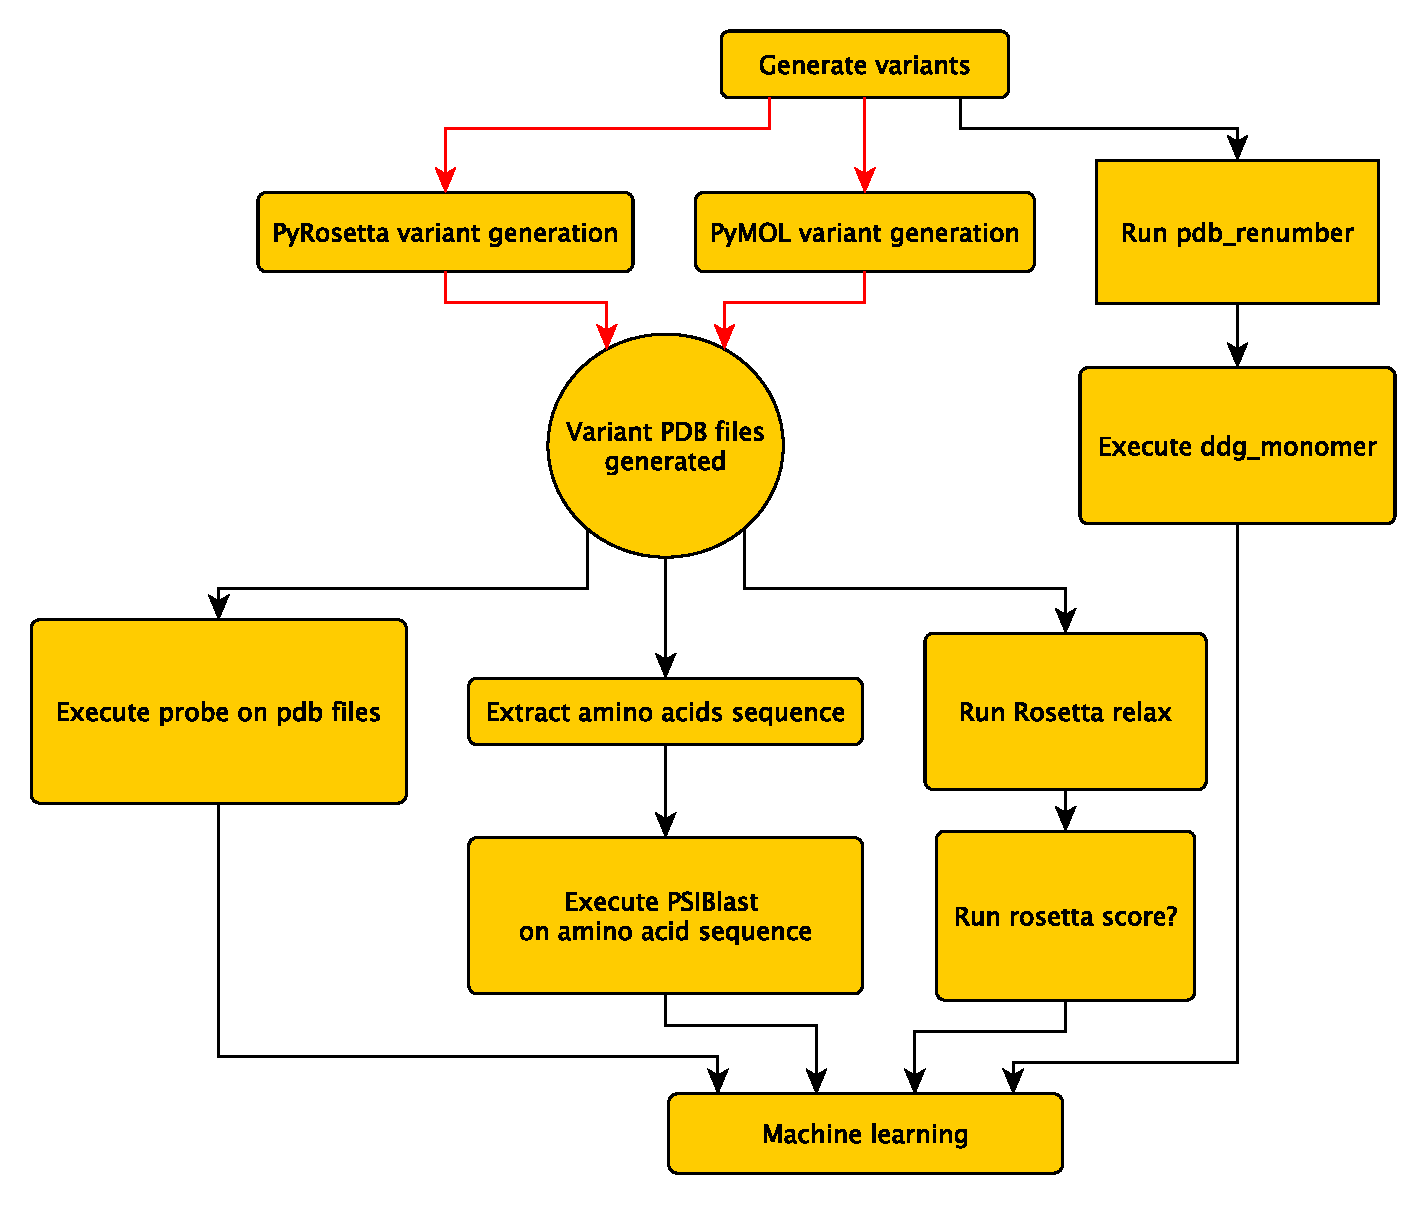
\includegraphics[width=\textwidth]{Flowcharts/VIPUR_approach.pdf}{a}
			\phantomcaption
			\label{fig:RES_VIPUR_approach}
		\end{subfigure}
		\begin{subfigure}{0.45\textwidth}
			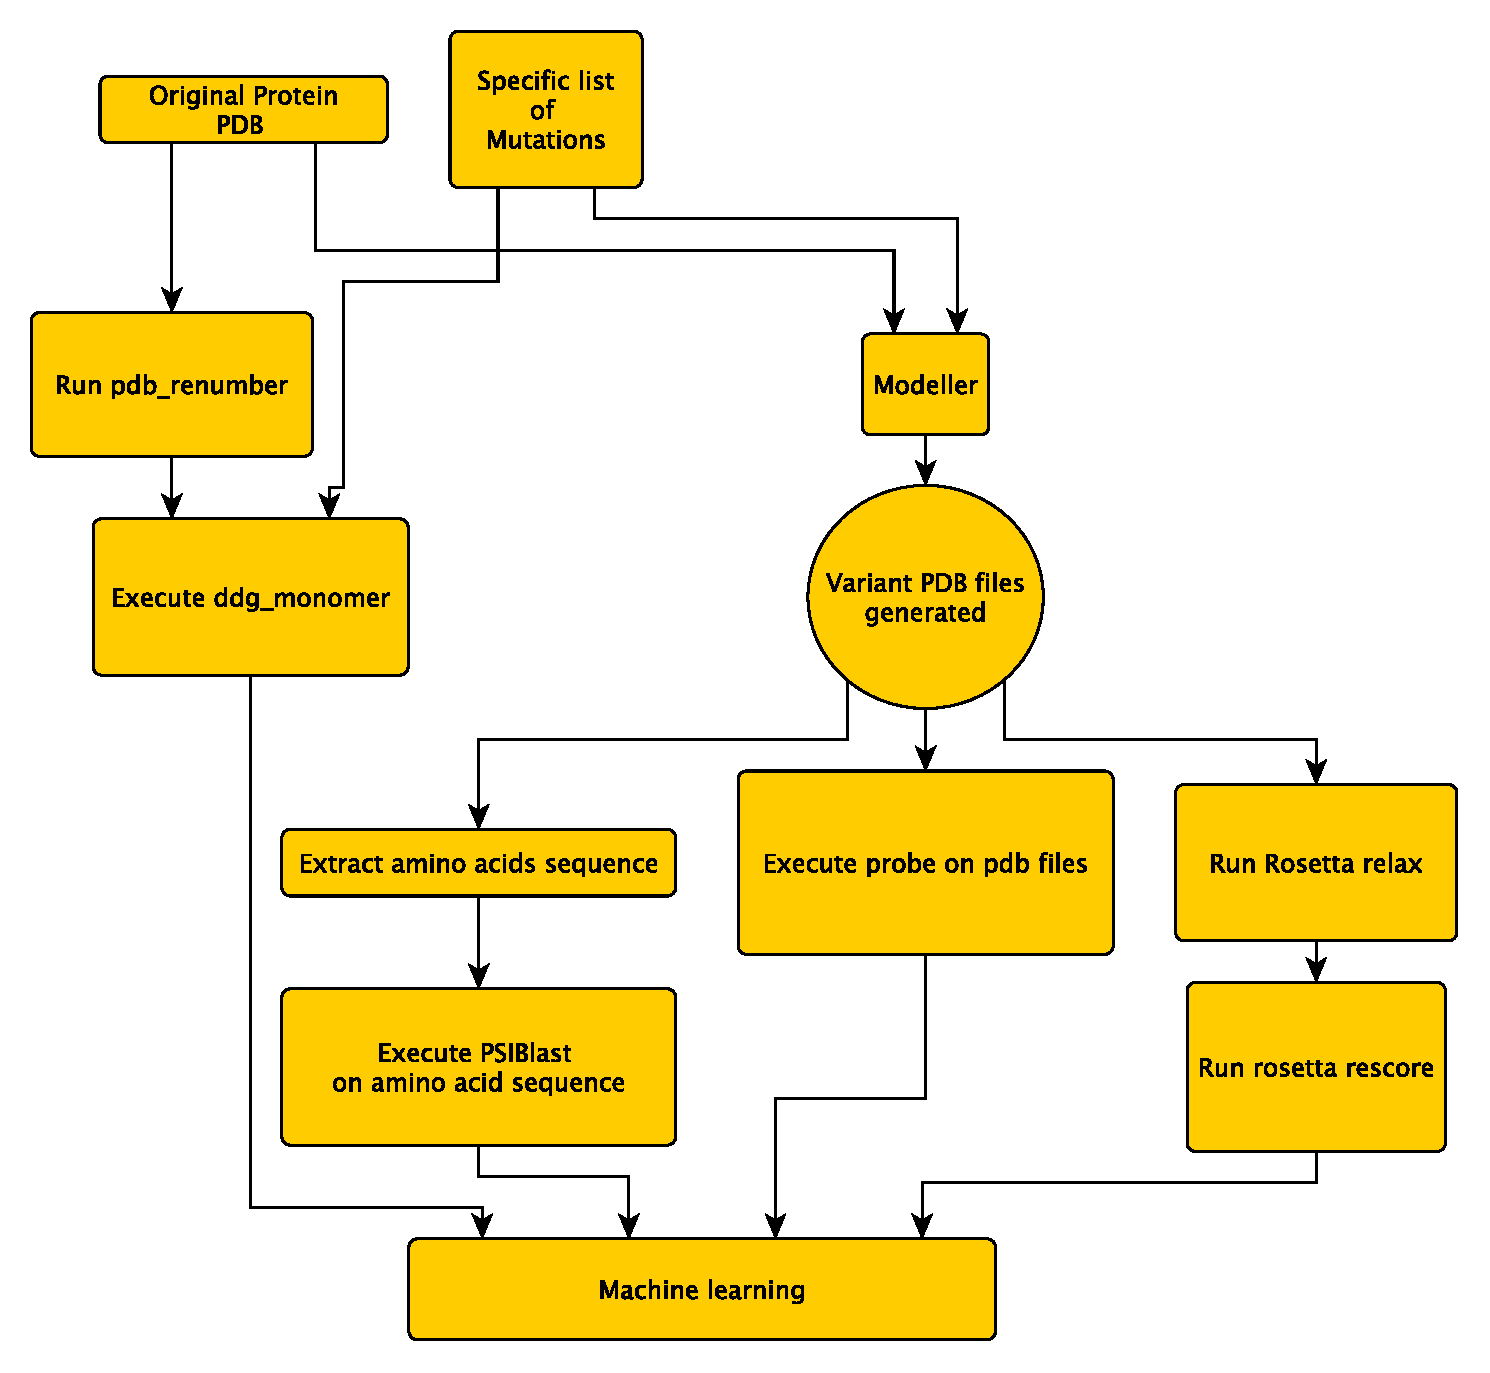
\includegraphics[width=\textwidth]{Flowcharts/Altered_VIPUR_approach.pdf}{b}
			\phantomcaption
			\label{fig:RES_Altered_VIPUR_approach}
		\end{subfigure}
		\caption[Flowcharts VIPUR pipeline and altered VIPUR pipeline]{Both flowcharts illustrate the VIPUR pipeline wherein each block is a procedure the central circle is the purpose of the mutated applications and each arrow represents the path to it. Figure \ref{fig:RES_VIPUR_approach} has red arrows that indicate that both methods were incapable to produce the mutated PDB files. Within figure \ref{fig:RES_Altered_VIPUR_approach} the alternative method is proposed wherein PyMOL and PyRosetta (Sections \ref{subsec:MM_PyMOL}, \ref{subsec:MM_PyRosetta}) is substituted by Modeller (Section \ref{subsec:MM_Modeller}) to acquire the mutated protein structures.}

		\label{fig:Flowcharts_of_old_and_altered_VIPUR}
	\end{figure}
	\label{subsubsec:RES_Incompatibility}
	\newpage
	
	\subsubsection{Expanding the VIPUR training set with data from TNFRSF1A by homology modeling and protein threading}
	Since the VTS did not have any features of TNFRSF1A (Section \ref{subsec:CD_TNFRSF1A}) the amino acid sequence was collected from Uniprot (Section \ref{subsec:MM_Uniprot}) and the protein from RCSB (Section \ref{subsec:MM_RCSB}). The structures available of TNFRSF1A were incomplete, fragments for the TNF $\alpha$ and $\beta$ binding site \cite{} were available and its death domain that interacts with TRADD \cite{} which plays a role in apoptosis (Section \ref{subsec:CD_TNFRSF1A}). To acquire a monomeric structure of TNFRSF1A two ab initio modeling web services I-TASSER and Robetta (Sections \ref{subsec:MM_I_TASSER}, \ref{subsec:MM_Robetta}) had been employed. Both were given the task to model the whole protein with and without a template to determine how well they could model a known structure and what it would form. Determination of the best model was based on the smallest root mean square deviation distance (RMSD )in {\AA} , between a produced model compared to the X-ray crystallographic model of the TNFRSF1A binding site.
	
%	Solution structure of the tumor necrosis factor receptor-1 death domain, Sukits
	\begin{figure}[!ht]
		\centering
		\begin{subfigure}{0.45\textwidth}
			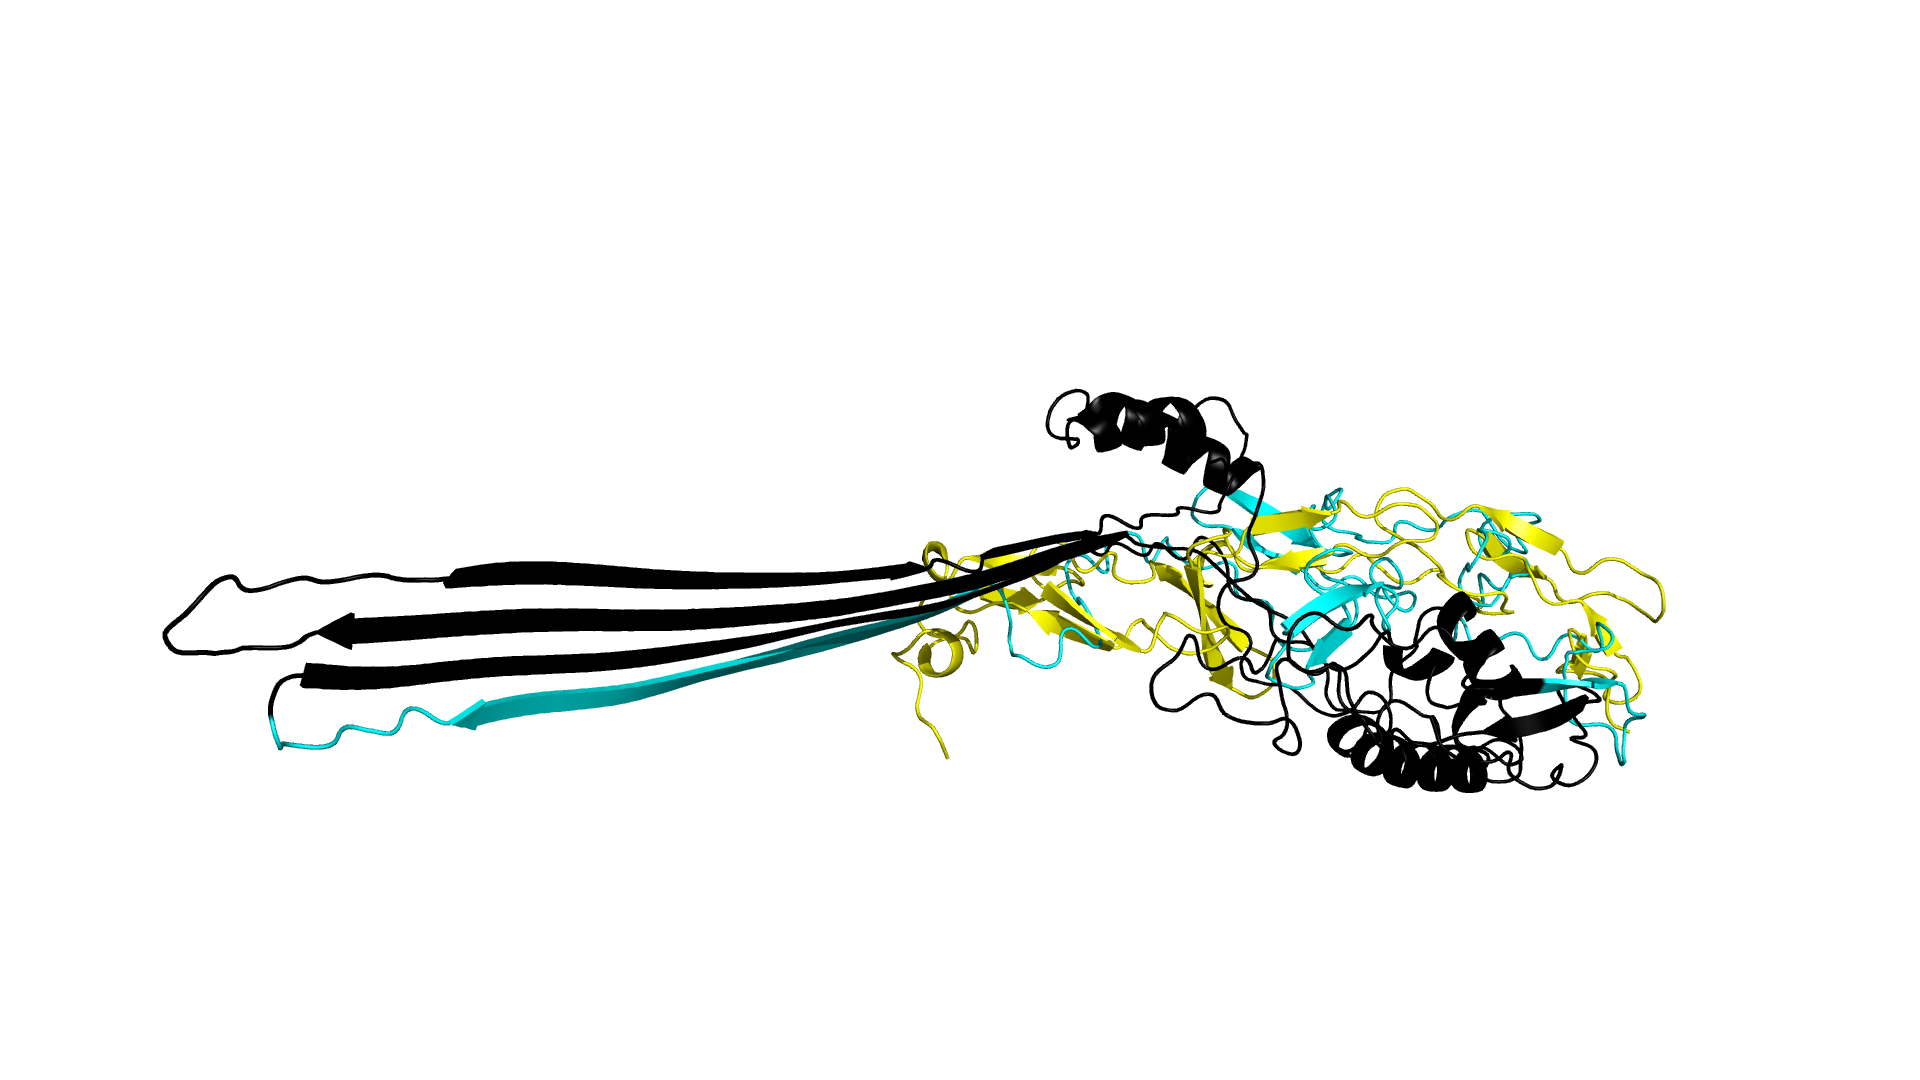
\includegraphics[width=\textwidth]{I_TASSER_Robetta_Images/1_EXT_ALIGN_I_TAS_WITHOUT_TEMPLATE.png}{a}
			\caption{RMSD = {\AA} 28.786}
			\label{fig:RES_I_TASSER_Without}
		\end{subfigure}
		\begin{subfigure}{0.45\textwidth}
			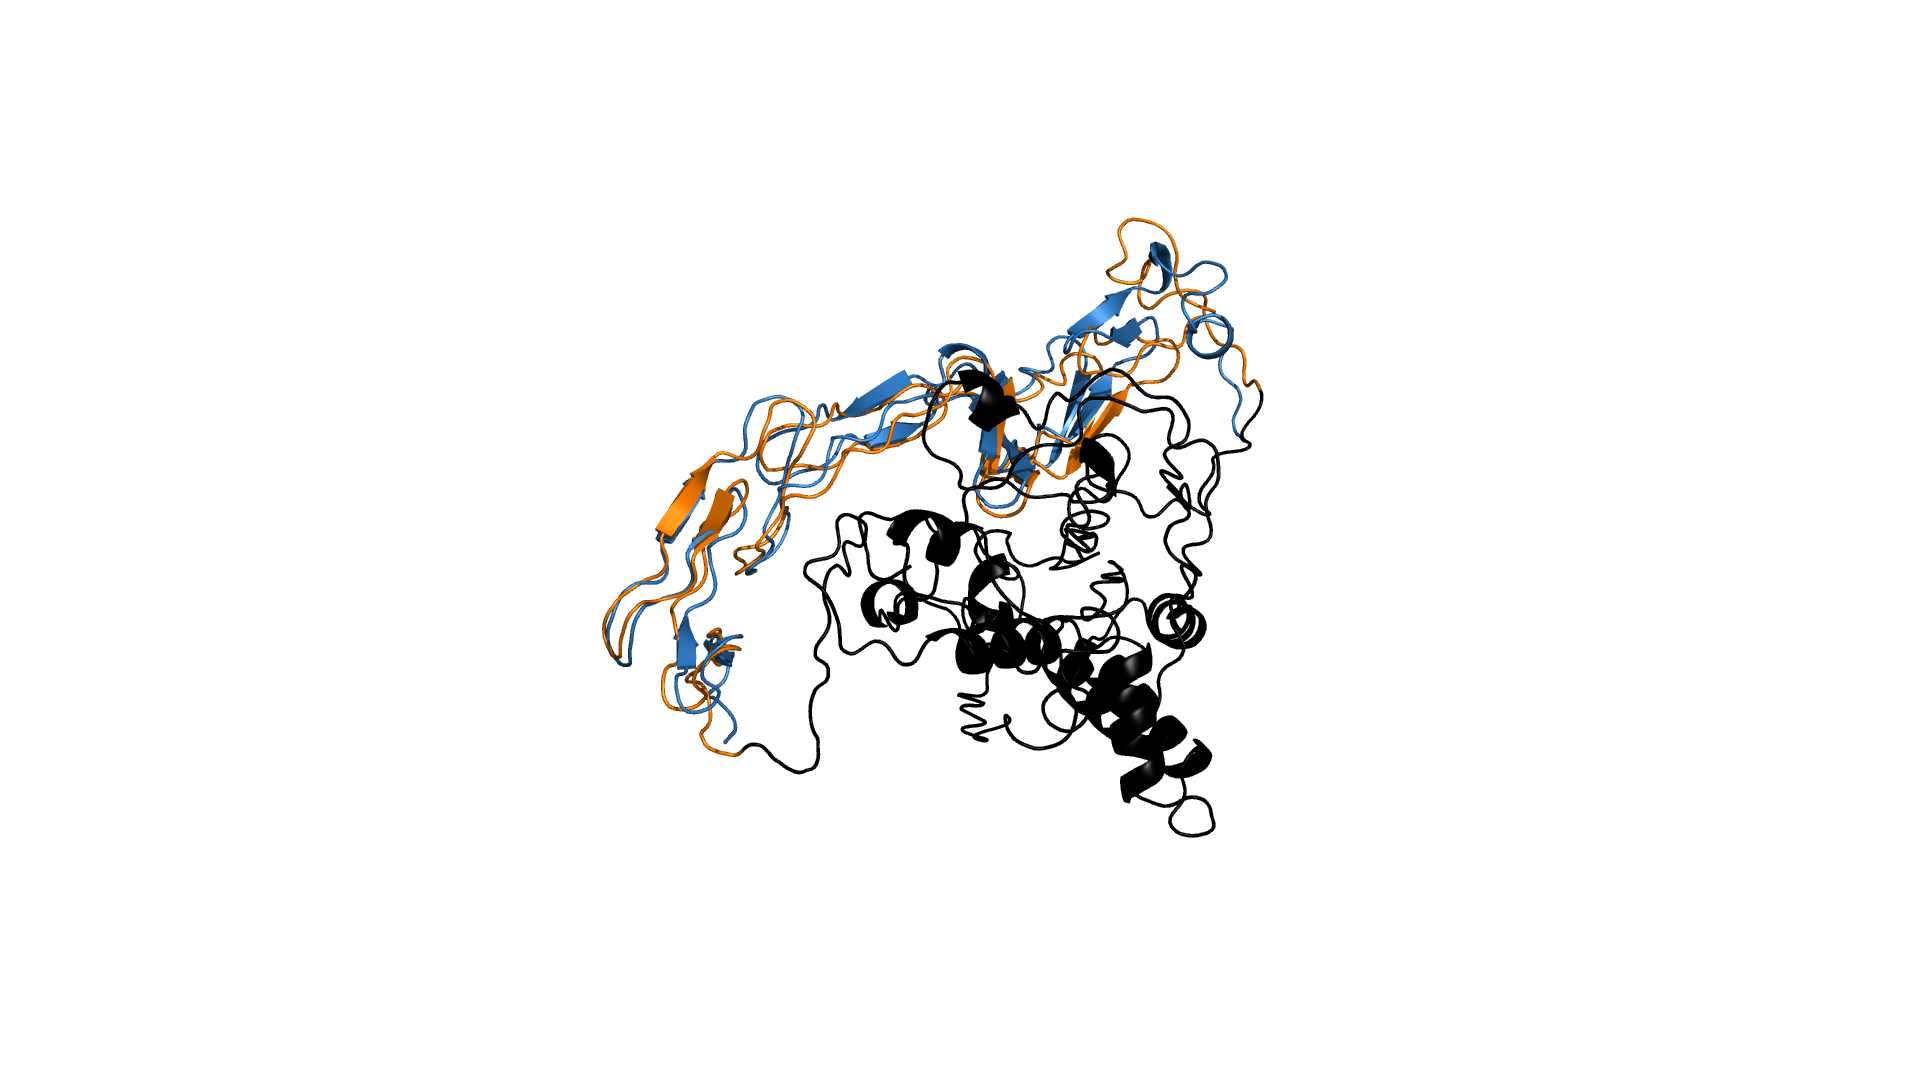
\includegraphics[width=\textwidth]{I_TASSER_Robetta_Images/1_EXT_ALIGN_I_TAS_WITH_TEMPLATE.png}{b}
			\caption{RMSD = {\AA} 3.830}
			\label{fig:RES_I_TASSER_With}
		\end{subfigure}
		\begin{subfigure}{0.45\textwidth}
			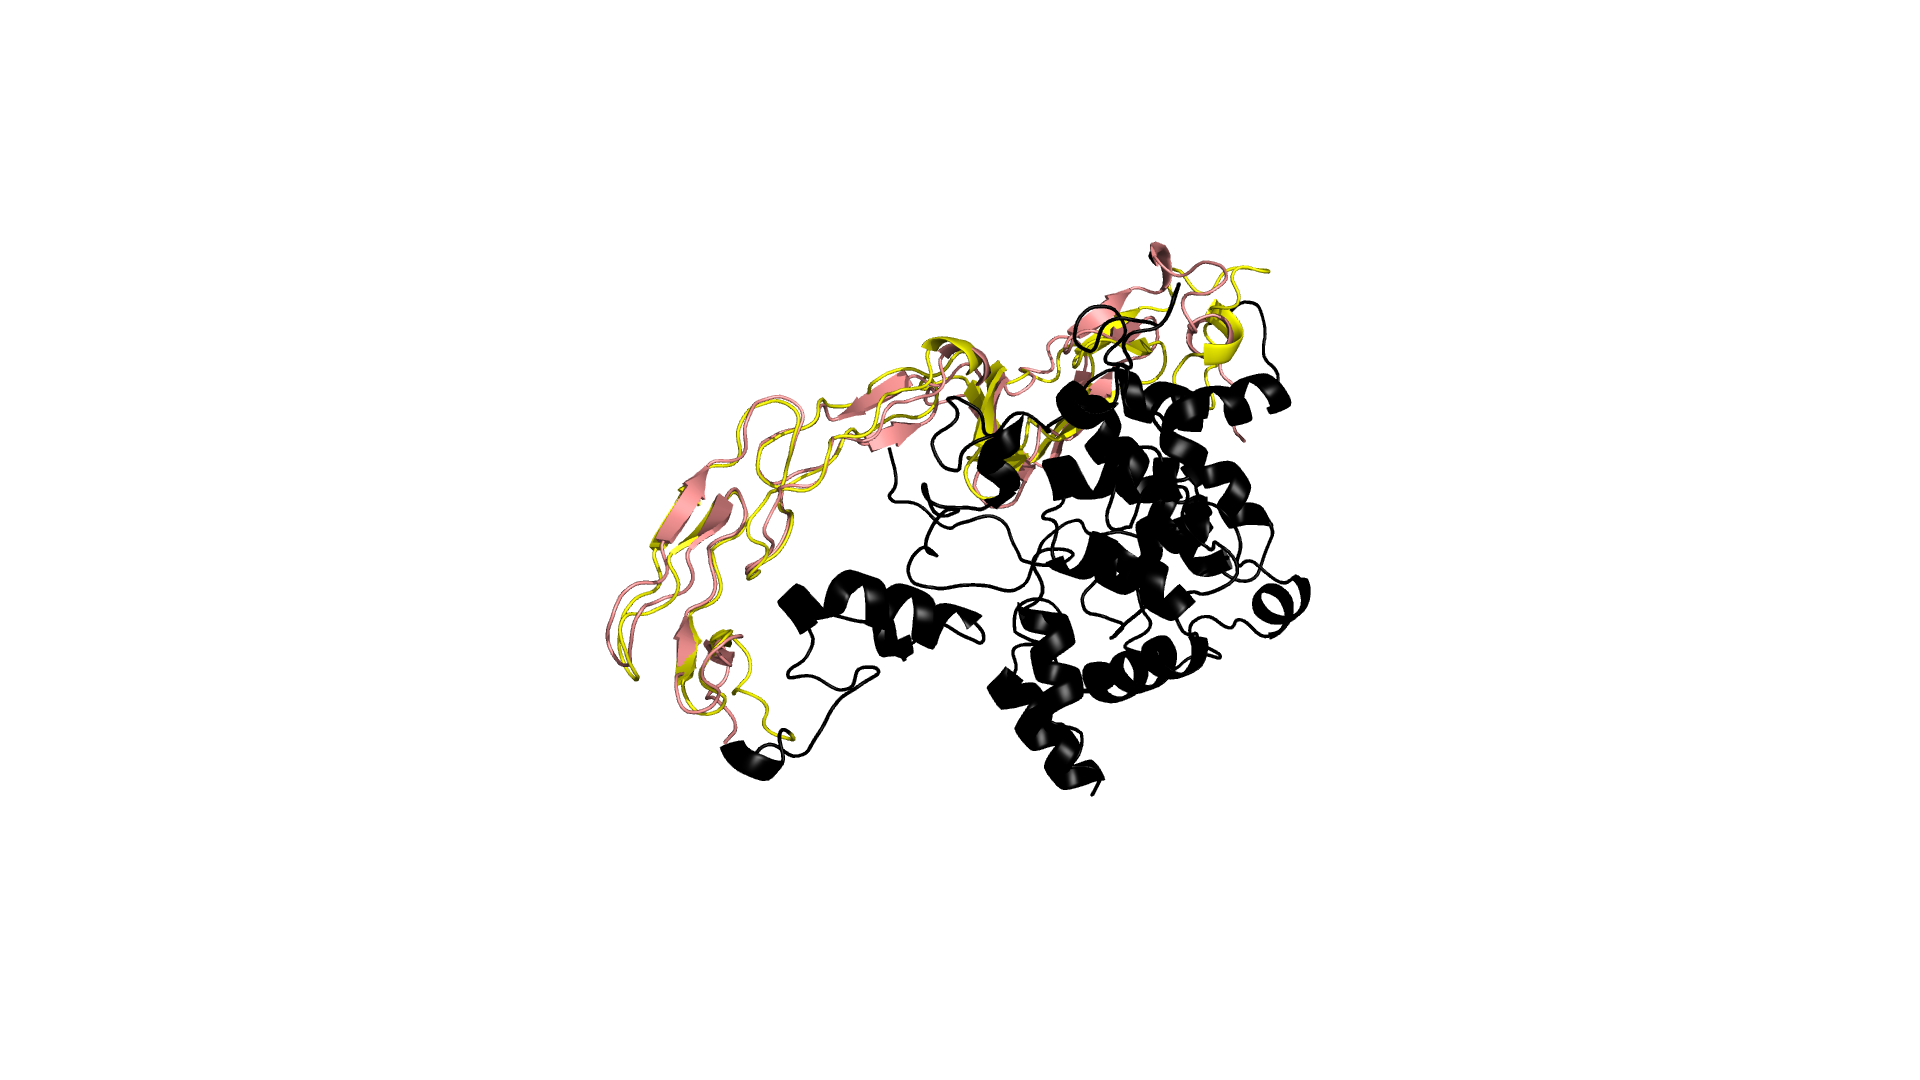
\includegraphics[width=\textwidth]{I_TASSER_Robetta_Images/1_EXT_ALIGN_ROB_WITHOUT_TEMPLATE.png}{c}
			\caption{RMSD =  {\AA} 3.067}
			\label{fig:RES_Robetta_Without}
		\end{subfigure}
		\begin{subfigure}{0.45\textwidth}
			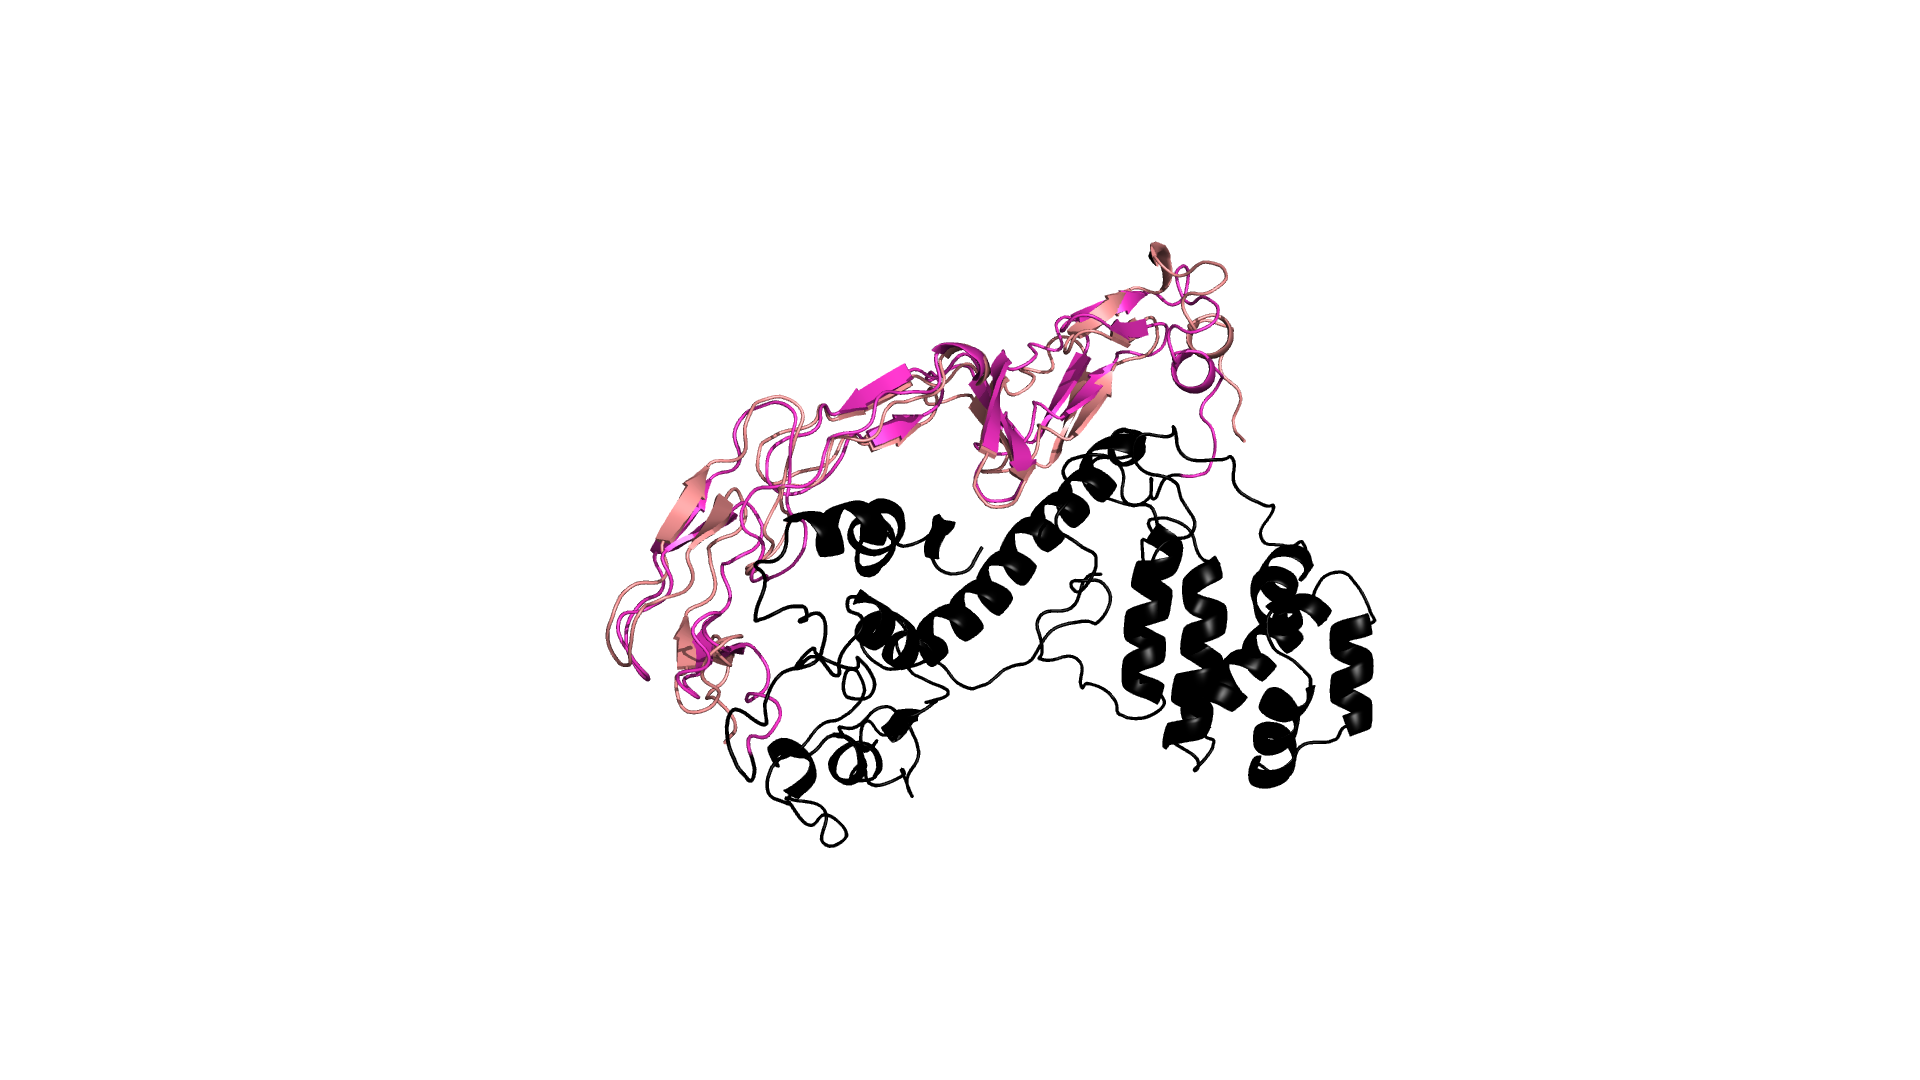
\includegraphics[width=\textwidth]{I_TASSER_Robetta_Images/1_EXT_ALIGN_ROB_WITH_TEMPLATE.png}{d}
			\caption{RMSD =  {\AA} 2.877}
			\label{fig:RES_Robetta_With}
		\end{subfigure}
		\caption[I-TASSER and Robetta models with and without templates]{3D structures of TNFRSF1A ( \ref{fig:RES_I_TASSER_Without}, \ref{fig:RES_I_TASSER_With}: I-TASSER, \ref{fig:RES_Robetta_Without}, \ref{fig:RES_Robetta_With}: Robetta) without (left: \ref{fig:RES_I_TASSER_Without}, \ref{fig:RES_Robetta_Without}) and with templates (right: \ref{fig:RES_I_TASSER_With}, \ref{fig:RES_Robetta_With}). The sky blue colored structure in each figure is an X-ray crystallographic model (1EXT) of the binding site of TNFRSF1A and the orange structure is the representation of that identical fragment in the model made by the web services.}
		\label{fig:I_Tasser_Robetta_models}
	\end{figure}
	\label{subsubsec:RES_Expanding_Models}

\newpage
\subsection{Analyses of proteins variants TNFRSF1A}
	\subsubsection{Requirements for determining structural and binding effects of protein variants}
	Protein variants can be assessed from multiple perspectives and together they can form a holistic view on how a protein works and how mutations affect its workings. However adding perspectives to the protein assessment makes it complex and requires expertise to determine its validity and contribution, therefore the analysis has been limited to basic structural information and also make the assessment inline with the VIPUR methods.
	
	Various proteins consist of multiple chains that can be identical or different depending on their function \cite{} and should be taken into account when assessing protein variants since one residue might alter the binding between chains and might alter the proteins formation. 
%	Lipin proteins form homo- and hetero-oligomers, Liu et al.
	Different molecules and atoms that do not make up a protein but play a role in a pathway and function (ligands and co-receptors) are able to affect a proteins shape and can behave differently when a residue is mutated. 
	
	A different aspect that can change with mutations is the alteration in motions between structures which can allow or disallow certain movements to occur and with inhibit processes.
	
%	In context of TNFRSF1A dimers that are formed when unbound can be altered by mutations and 
	
%	Other parts that alter to protein and play a role in function are ligands and co-receptors that 
%	To get the appropriate structural information of a protein 
%	
%	the informational search scope has been limited to structural information and 
%	
%	 therefore the search scope has been limited to structural information.
%	For structurally assessing protein variants a there are several requirements, 


%	SOMETHING ABOUT 1TNR and 1EXT!
%	Structural information of proteins describes how a protein functions and how it behaves within a cell, however it is difficult to analyze since
%	
%	Proteins variants can be assessed from different perspectives and all are necessary to 
%	Assessing protein variants and its effects 
%	
%	Assessing protein variants and the effects that a variant might cause can be assessed from different fields of view and could give a holistic view on problem that arise during mutations. However adding every perspective in an analyses is difficult because collecting all available information often has to be done manually and to determine which information is relevant requires expertise. However it can be complex to put all the information and since  
%	
%	
%	Because the VTS mainly consists of structural features and 
%	
%	To make assessment less complex and because the VTS has mainly structural features 
%	
%	 a structural point of view was taken for the protein TNFRSF1A 
%	
%	To simplify the complexity of the problem only a structural point of view with limited alterations was taken
%	
%	To simplify the problem it has been recapitulated into 
%	
%	the perspectives of form and function.
%	
%	The perspective of form describes how a protein takes shape based on the environment and amino acid sequence, within the context of TNFRSF1A it describes how dimer structures are formed on the cell surface when unbound and that it forms a trimeric structure when it is bound by TNF 
%	
%	Function determines how certain parts of a protein behave within an environment and determine its effects on a pathway. 
%	
%	In context with TNFRSF1A one part resides on the cell surface where it binds ligands and on the cytoplasmic side it can interact with protein that triggers an inflammatory response or apoptosis. When a mutation is introduced at the cell surface side it might not be able to form dimer formations that interact with TNF ligands or during transformation with the binding of TNF it is unable to bind trimers. 
%	
%	Wherein the perspective of form the deciding factors are the amino acid sequence and where it resides within the cell.
%	
%	A different perspective is form wherein the amino acid sequence determines how a protein structure will be formed.
%	
%	Before the moment of writing no protocol was available which dealt with structural variation 
%	
%	Currently there is no protocol available to asses protein variants with structural information, 
	
%	Assessing protein variants and its effects should be studied with a multidisciplinary view wherein form and function are assessed. Within the aspect of form should be seen how a protein is formed
%	
%	
%	However due to difficulties with experiments it can be hard to unravel all the effects that can be caused by mutations.
%	
%	 A part of this view is to know what function the protein has before its mutated to determine its effect on a pathway or function. 
%	
%	How does the 
%	
%	
%%	 Effect
%	Can a cell or pathway still function without this protein? or is there an alternative mechanism within the cell that is less efficient in performing similar role? 
	
	\subsubsection{Single protein variant analysis approach and its tools}
	Before introducing mutations into a protein structure it is helpful to know if a mutation has been observed to avoid allocating resources to something that does not occur. Therefore three tables with observed TNFRSF1A mutations (Sections \ref{subsec:MM_GAVIN_data_table}, \ref{subsec:MM_GnomAD}, \ref{subsec:MM_Infevers}) have been combined with an R script (Section \ref{subsec:MM_R}) into a single table consisting of two columns. The first column (split into three columns \ref{table:Res_Filtered_Mutations}) contains strings that describes the: original residue, position and where it mutates to, the second column describes whether a formed mutation is harmful, with most mutations the effects have not been identified yet. 
	\begin{table}[ht]
		\begin{tabular}{ l | l | l | l}
			Original residue & Position in the protein sequence & New residue & Classification\\ \hline
			Cys & 44 & Tyr & PATHOGENIC\\
			Thr & 44 & Pro & PATHOGENIC\\
			Thr & 44 & Ser & PATHOGENIC\\
		\end{tabular}
		\caption[Sample of combined tables with observed mutations]{The format wherein mutations were filtered from the GAVIN, GenomAD and Infevers tables (Sections \ref{subsec:MM_GAVIN_data_table},  \ref{subsec:MM_GnomAD}, \ref{subsec:MM_Infevers}),  describe whether a structural mutation is harmful or not. For many mutations it is unknown and other classifications are available, to view the whole table visit the supplementary.}
		\label{table:Res_Filtered_Mutations}
	\end{table}
	
	For assessing variants in TNFRSF1A a structural fragment was used that contained TNF $\beta$ (1TNR) \cite{} and was made homotrimeric with PyMOL (Section \ref{subsec:MM_PyMOL}) which results in six chains that emulate a bound TNFRSF1A with TNF $\beta$. The first column of the mutation table did not contain sufficient information to apply mutations correctly and within the PDB different numbering is used than in the amino acid sequence. To bundle the information and make it usable for introducing mutations a Python script (Section \ref{subsec:MM_Python}) has been written that combines the mutation table, PDB chains and the correct position within the sequence into a type of table which has sufficient information to mutate structures.  
	%	Crystal structure of the soluble human 55 kd TNF receptor-human TNFβ complex: Implications for TNF receptor activation, Banner et al. 
	\begin{table}[ht]
		\begin{tabular}{ l | l | l | l | l}
			Iteration number & Filename & Chain & Residue index in chain & New residue\\ \hline
			34 & 1tnr3\_TNFA & R & 0 & TYR\\
			34 & 1tnr3\_TNFA & T & 0 & TYR\\
			34 & 1tnr3\_TNFA & S & 0 & TYR\\
			35 & 1tnr3\_TNFA & R & 0 & PRO\\
			35 & 1tnr3\_TNFA & T & 0 & PRO\\
			35 & 1tnr3\_TNFA & S & 0 & PRO\\
			36 & 1tnr3\_TNFA & R & 0 & SER\\
			36 & 1tnr3\_TNFA & T & 0 & SER\\
			36 & 1tnr3\_TNFA & S & 0 & SER\\
		\end{tabular}
		\caption[Sample of table with applicable missense mutations to TNFRSF1A]{The format that describes the mutations that should be made by Modeller (Section \ref{subsec:MM_Modeller}), with specifications of the: model, file. chain, residue index and the new residue. The whole table for TNFA and TNFB are visible within the supplementary.}
			\label{table:Res_Modeller_Mutation_Format}
	\end{table}
	
	\newpage
	To introduce mutations within PDB structures a Python script (Section \ref{subsec:MM_Python}) was written which used the generated mutation table (Table: \ref{table:Res_Modeller_Mutation_Format}) and a matching PDB structure, from the table; it acquires an iteration number which specifies if a mutation has to be stored in a single file or across multiple files; the filename serves as key which determine the PDB that should be used; letters specify chains, numbers are indices within the chains and the last column states the three letter residue where it should mutate to. When a structure is read in through the Python bindings of Modeller (Section \ref{subsec:MM_Modeller}) all non standard atoms and molecules are removed because Rosetta (Section \ref{subsec:MM_Rosetta}) is not able to deal with those atoms. Just before mutagenesis takes place missing atoms are added to the structure that were difficult to determine with experimental methods(Section \ref{subsec:GD_Addition_of_structural_data}). After the insertion of all mutations a last guess is made where disulfide bonds are added between cysteines. With this process variants can be easily made, however the mutations do not present a correct protein because the mutated residues can put the protein in a high energy state.
	
	In the attempt to make mutated structures behave more natural two tools from the Rosetta software suite (Section \ref{subsec:MM_Rosetta}) have been used to minimize energies within protein structures. With the backrub application (Section \ref{subsubsec:MM_Backrub}) 1000 altered backbone models have been produced each with 10000 Monte Carlo moves (Sections \ref{section:Chap_Monte_Carlo}). Each model generated has a set of properties that describe the formed molecule 
	
	Relax? 
	
	We specifically chose to asses known mutations from infevers.?
	Density goes beyond 1?
	
	
	\newpage
	\begin{figure}[!ht]
		\centering
		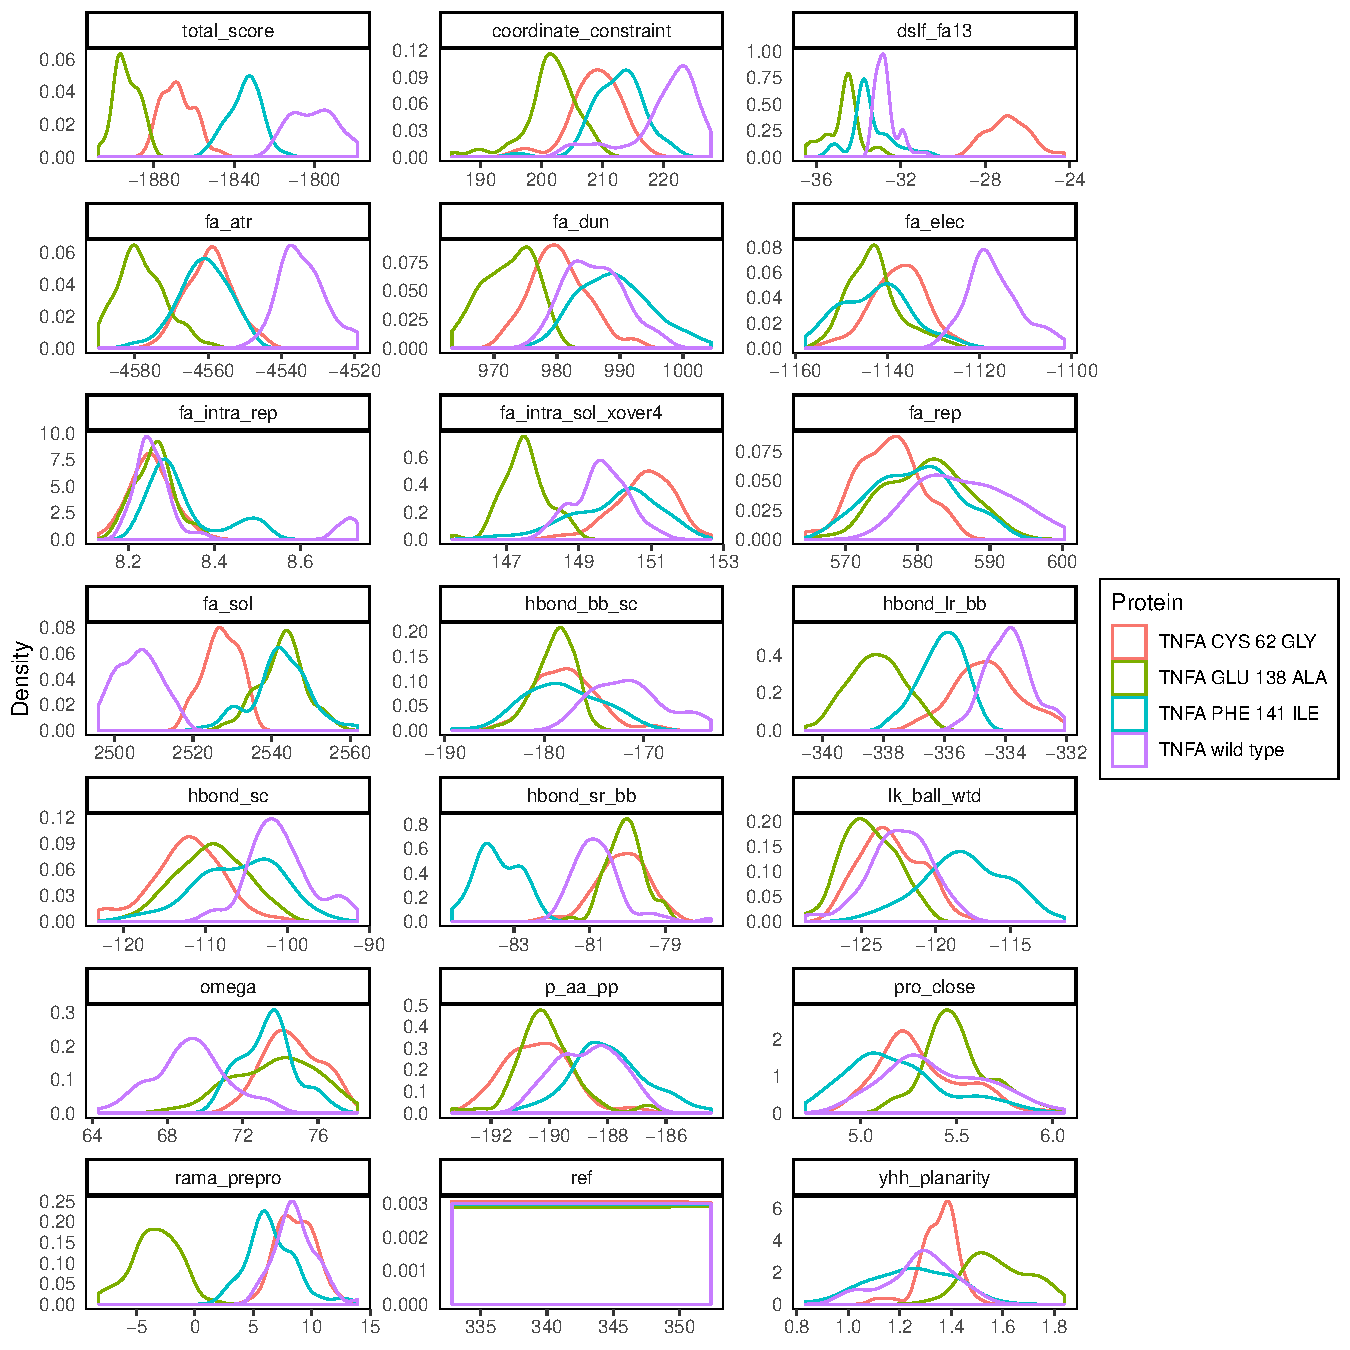
\includegraphics[width=\linewidth]{Rosetta_Backrub_Relax_Density_Plots/relax_Alpha_plot.pdf}
		\caption[TNF-$\alpha$ relax score plots]{}
		\label{fig:relax_TNFA_scores}
	\end{figure}

	\newpage
		
	\begin{figure}[!ht]
		\centering
		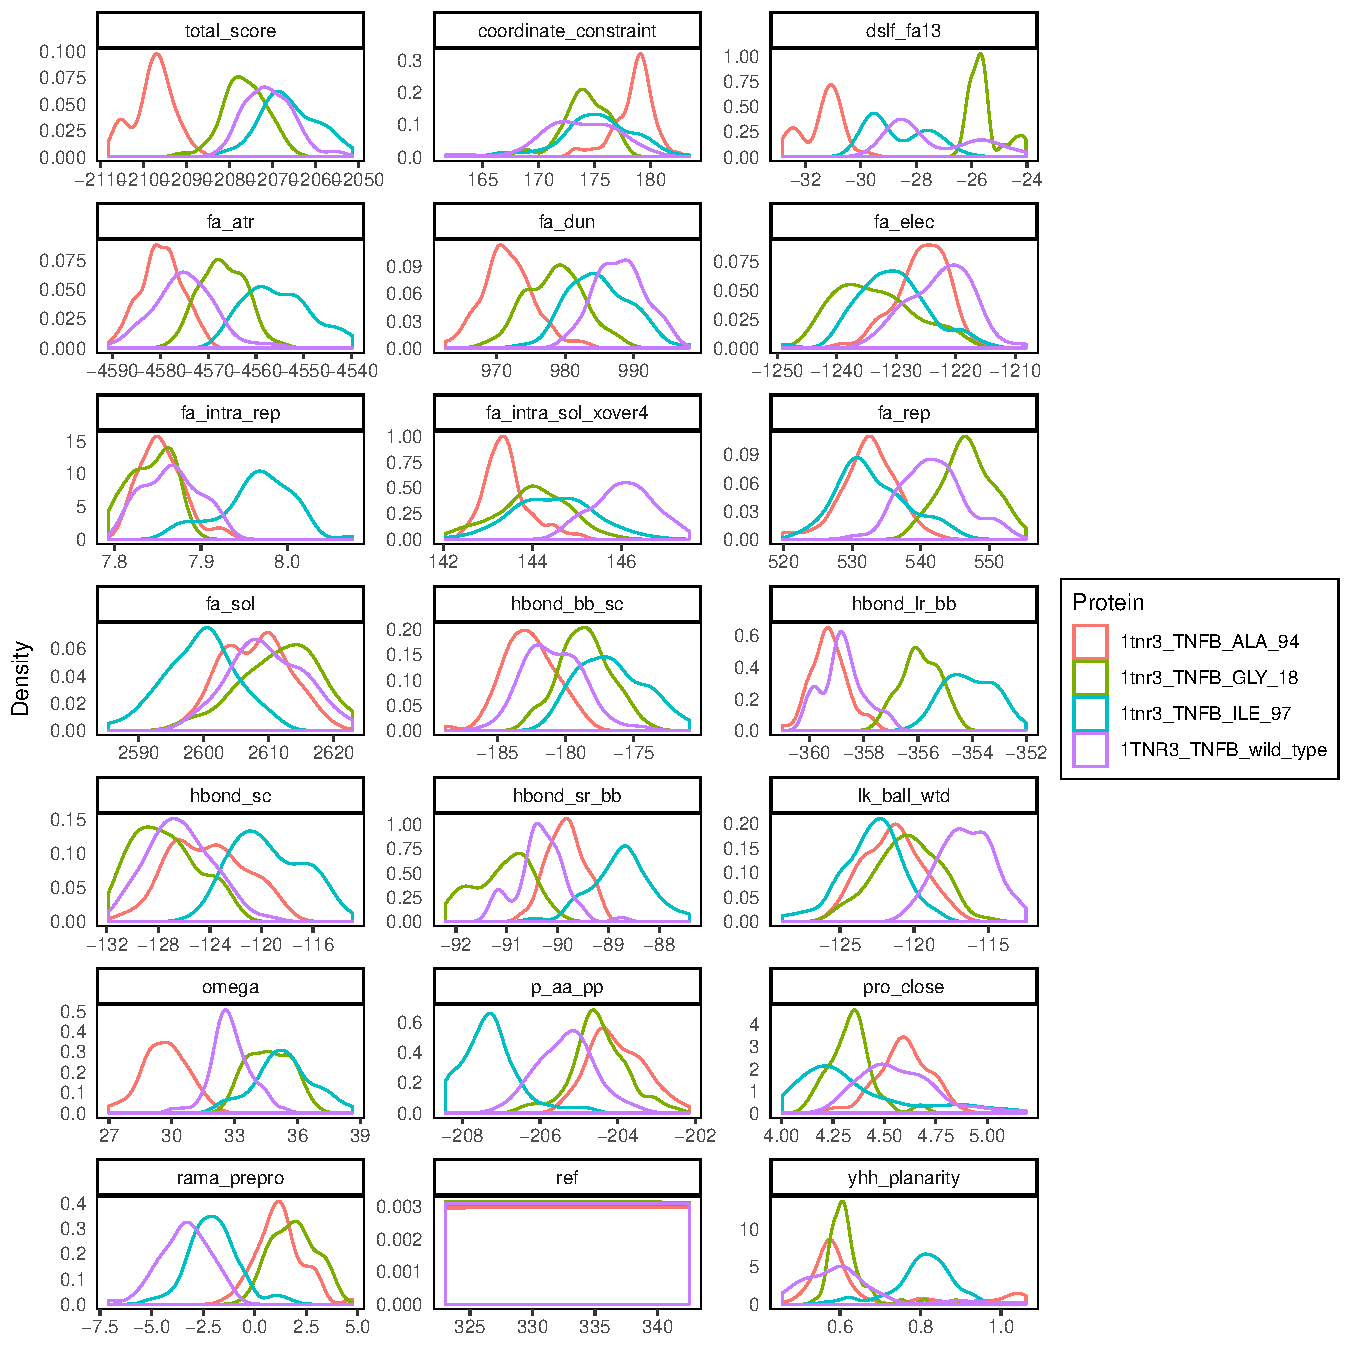
\includegraphics[width=\linewidth]{Rosetta_Backrub_Relax_Density_Plots/relax_Beta_plot.pdf}
		\caption[TNF-$\beta$ relax score plots]{}
		\label{fig:relax_TNFB_scores}
	\end{figure}

	\newpage
	
	
	
\newpage	
\subsection{Finding structural information and its mutations through HOPE}
	With uncertainty in the numbers provided by SPVAA a more textual informative approach was used with the web service HOPE (Section \ref{subsec:MM_HOPE}). The mutations that were known from Infevers (Section \ref{subsec:MM_Infevers}) and were also used with SPVAA were tested by HOPE (CYS62GLY, GLU138ALA and PHE141IlE), all reports are visible within the supplementary.
	
	HOPEs first test was the mutation of Cysteine 62 to glycine, which is known within the Infevers table as pathogenic and was validated. It discovered that the residue was involved in a disulfide bridge and was 100\% conserved in related protein sequences, based on the observation that cysteine formed a disulfide bridge it expected that with te replacement of it glycine would make the whole structures less rigid. HOPE predicts that mutation is pathogenic because of the high conservation of the residue, which is further confirmed by its search results in which if found the original publication where the observation has been described and associated to TRAPS \cite{}.
%	The tumor-necrosis-factor receptor-associated periodic syndrome: new mutations in TNFRSF1A, ancestral origins, genotype-phenotype studies, and evidence for further genetic heterogeneity of periodic fevers, Aksentijevich
	
	According to Infevers is the mutation of glutamic acid at position 138 mutated to alanine classified as likely benign and was not validated yet. HOPE discovered with a BLAST query that glutamic acid occurs often at position but other residues such as alanine have been observed at the position. Structurally glutamic acid forms salt bridges with proline  368 and leucine 390 and is found in a sequence of amino acids that is repeated through out TNFRSF1A. The amino acid lies within a domain where it interacts with other domains and is important for the proteins activity, with this mutation it might already perturb the binding capabilities according to HOPE.
	
	The last mutation that was tested with HOPE was phenylalanine 141 to Isoleucine and was according to Infevers pathogenic and has been validated. Phenylalanine has been conserved at this positions and few other residues have been seen at the position, it is member of the identical domain as glutamic acid 138 and HOPE predicts that it would not damage the protein based on this information. However within the structure it could inhibit interaction with other domains and protein activity.
	
	
%	
%	
%	 to arrange this information properly a Python script (Section \ref{subsec:MM_Python}) used the files and
%	
%	 and the exact position within the PDB file (1TNR) had to be added with a Python script (Section \ref{})
%	
%	 were introduced with a Python script (Section \ref{subsec:MM_Python}) wherein  and had to be introduced with  Introducing mutations in the trimeric mol
%	
%	Each of wherein mutated 
%	
%	
%	
%	three mutations in separate structures were introduced.
%	
%	The mutation tables first column is insufficient and requires additional information regarding TNFRSF1A chains to make mutations in TNFRSF1A, information regarding the chains 
%	
%	From the mutation table only information of the first column is used to make alterations in structural models, that part of the table will play a role in modifying protein structures with Modeller (Section \ref{subsec:MM_Modeller}). Because the model is homotrimeric it has multiple poly peptides chains that all need to be modified without modifying the ligand. 
%	
%		
%	
%	 But more information is required to make a new format, since TNFRSF1A is a homotimer a
%	the function of the mutated protein is within a pathway 
%	A broad perspective should be taken with a 
%	To determine the effects of mutated residue awithin a protein variant a b than structural information should
%	Up until VIPUR and the development of similar approaches that benefit from structural information

%
%
%
%Something about that we tried to use the VTS and add our protein for information.




	\label{section:Chap_Results}
	\newpage
	
	\section{Discussion}
	%INTRO
People with rare diseases are currently hard to diagnose and are often not put in the desired treatment groups, with machine learning methods such as GAVIN 95\% of the benign variants can be harmfully removed, however these methods rely on conservation and have been heavily optimized over the years \cite{}.
%GAVIN: Gene-Aware Variant INterpretation for medical sequencing, van der Velde
A new refreshing approach called VIPUR uses sequential and structural data to predict deleteriousness of a protein variants.

%VIPUR
Within the attempt to make VIPUR usable for the diagnosis of rare diseases it was discovered that some questionable steps were taken to make it especially applicable for diagnosis but also to determine deleteriousness of proteins itself: (i) "All protein models were standardized to remove unwanted components (duplicate chains, ligands, metals and non-standard amino acids)" \cite{}.
%Robust classification of protein variation using structural modelling and large-scale data integration, Baugh
Standardizing data can be beneficial to avoid learning features that do not matter and can reduce overfitting. However any form of context to the protein is removed and might therefore make incorrect assumptions about how: a monomer interacts with other monomers, ligands, metals, non-standard amino acids and water which can all have an effect on how proteins shape and interact \cite{}.
%Application of a Theory of Enzyme Specificity to Protein Synthesis*, Koshland
(ii) With the utilization of Rosetta's Relax application different models are formed based on the Monte Carlo method (Section \ref{section:Chap_Monte_Carlo}), VIPUR produces 50 structures with Relax per protein which is a tiny amount of the potential search space of possible folds that could have made changes in a mutated protein, which also can be seen in the scores of the model made from of TNFRSF1A with TNF $\alpha$ \& $\beta$ (Figures \ref{fig:relax_TNFA_scores}, \ref{fig:relax_TNFB_scores}), Rosetta itself suggests to make sufficient models, starting with 5000\cite{}.
%Analyzing Results, Rosetta commons
(iii) The features acquired with probe in combination with the models that were produced, within the publication of Probe is mentioned: "It requires both highly accurate structures and also the explicit inclusion of all hydrogen atoms and their van der Waals interactions." \cite{}.
%Visualizing and quantifying molecular goodness-of-fit: small-probe contact dots with explicit hydrogen atoms11Edited by J. Thornton, Word et al.
It is currently not possible to determine if the structures were accurate, however is it likely that no loose hydrogen atoms were included within the structure based on the knowledge that all structures were standardized and likely some of the structures did not have any loose hydrogens within them. To make the outcome of Probe useful to VIPUR the program Reduce should have ran first, which add hydrogen atoms to the structure, which is recommend on the site were Probe can be downloaded from \cite{}.
%Probe Software : Kinemage Website, Richardson LAB
%The site of Probe mentions: "Meaningful analysis of molecular contact surfaces requires that ALL atoms are considered. Before using Probe, use the companion program Reduce to add hydrogens to the coordinate file." \cite{}, no mention of the Reduce software is mentioned in the VIPUR approach and therefor it is difficult to asses the meaning of previously acquired results in the VTS.

? easy pick ?
Within Figure 4 of Robust classification of protein variation using structural modelling and large-scale data integration \cite{} is stated that the mutation on position 204 from serine to proline is predicted deleteriousness, which is even without assessment highly likely because as can been in the structure it resides within an $\alpha$ helix and proline is known as the helix-stopper \cite{}.
%Robust classification of protein variation using structural modelling and large-scale data integration, Baugh
%Alpha-helical, but not beta-sheet, propensity of proline is determined by peptide environment, Li et al.

VIPUR was not tested because of; several compilation issues related to libraries making not possible to compile PyMOL or PyRosetta (Sections \ref{subsec:MM_PyMOL}, \ref{subsec:MM_PyRosetta}), not able to run since it was made specifically for a single system and by modifying it unable to execute the basic implemented demo and due to the lack of time to reverse engineer Modeller (Section \ref{subsec:MM_Modeller}) into VIPUR. 


Based on the figures (4, 5) \cite{} and supplementary figures (10,11) \cite{} there is a suspicion that there is little added value to the structural information within VIPUR and the predictions made by VIPUR depend on the results of PSI-BLAST.
%Robust classification of protein variation using structural modelling and large-scale data integration, Baugh et al.
%SUPPLEMENTARY: Robust classification of protein variation using structural modelling and large-scale data integration, Baugh et al.
To determine if this is the case it should be tested with methods that determine the contribution of features that are used by VIPUR.


Good other suggestions for finding if the approach really means something is by using shap \cite{}.
%slundberg/shap: A unified approach to explain the output of any machine learning model, Slundberg
%Explaining Prediction Models and Individual Predictions with Feature Contributions, Štrumbelj
%Why Should I Trust You?": Explaining the Predictions of Any Classifier, Ribeiro
%Learning Important Features Through Propagating Activation Differences, Shrikumar
%Algorithmic Transparency via Quantitative Input Influence: Theory and Experiments with Learning Systems, Datta
%On Pixel-Wise Explanations for Non-Linear Classifier Decisions by Layer-Wise Relevance Propagation, Bach
%Interpreting random forests | Diving into data, Datadive

% ASSUMED
VIPUR uses PSI-blast to justify its results. 

% Compilation issues
With the resource at our disposal we were unable to reproduce any of the results that were produced by VIPUR for testing purposes.
The VIPUR pipeline could not be executed because it was not possible to compile PyRosetta or PyMOL on the cluster.

%adquate thing about VIPUR quartiles
A good thing from VIPUR is that they took the information of all samples, it might introduce errors but also excludes lowers the extremes and might make it more realistic.



% last part of VIPUR
With Monte Carlo methods under te hood of the relax application it  such as relax it is beneficial to produce many models since it is
Although it is not part of developing a technique that can help diagnosing rare disease variant but the publication contains a claim ("VIPUR can be applied to mutations in any organism’s proteome...." \cite{}) that likely contradicts with its methods ("remove unwanted components (duplicate chains, ligands, metals and non-standard amino acids)" \cite{}). There are 20 amino acids classified as standard, 22 are known to be incorporated into structures of some organisms \cite{} and more variants are possible, which makes it unclear what is classified as a non-standard amino acid.
%Robust classification of protein variation using structural modelling and large-scale data integration, Baugh
%Natural expansion of the genetic code, Ambrogelly et al.




% SPVAA
SPVAA method show similar weaknesses as VIPUR, it removes metal and water but keeps the ligands and are even added when necessary.

We did not asses the whole in a complex because there was insufficient information. (Membrane, water, other atoms and we could have left some atoms that were not water.)

With SPVAA only looked at the trimeric form an not the dimeric form of TNFRSF1A.
Only using the Rosetta energy to determine the effect of the protein.

Isoforms were not taken into account.

Only assessed a small piece of TNFRSF1A and did not even look at the class of proteins itself.

With the resource at our disposal  limited.
More iterations on Rosetta relax than 64\cite{}.
%Analyzing Results, Rosetta commons

The software written has a limited use currently and could be expanded to rapidly introduce mutations in multiple structures and chains at once.

It might have been useful to disable disulfide bridges if no cysteine residue is mutated because it is less likely that alterations are formed to disulfide bridges and otherwise they might be added without a reason.

Fragments were only available of 1EXT and 1TNR because it is a transmembrane protein which is difficult to make a structure from with X-ray crystallography.
Maybe the first 30 residues were unnecessary because the might be signal peptides. 

%HOPE
HOPE is informative with the results it produces, easy to use, fast and makes structural problems within proteins diagnoseable and understandable when a missense mutation is discovered. However it does not draws a solid conclusion and the information it collects depends on: previous publications, conservation and experimental structures, which will give it a disadvantage when limited knowledge is available. Also it does not asses a complex but it can describe binding sites from the monomer when previously discovered.


% MOLECULAR DYNAMICS
SPVAA's assement and VIPURs prediction could potentially be improved with the addition of molecular dynamic simulations to determine the effects of structural changes. With SPVAA it would have most likely become clear if the loss of the disulfide bridge from cysteine 62 in TNFRSF1A would have caused structural issues. VIPUR could benefit from it as new machine learning feature in situations where limited movement is observed and it changes tremendously when a missense mutation occurred in a protein increases with a mutation or vice versa.



% General problem with all methods
All methods are reliant on existing structures making it difficult to asses it as a complex.

	\label{section:Chap_Discussion}
	\newpage
	
	\section{Conclusion}
	VIPUR is missing information to give a solid prediction about the deleteriousness of a protein variant and therefore likely suffers from errors in the predictions, SPVAA which uses changes in energy levels could be a more reliable source but also shows its weaknesses within the pace it can asses protein variants, it makes the determination manual and requires background knowledge for the assessment of protein variants. 

 of info that accurate we propsed another method for assessing protein structures within complex which may play a role in machine learning
 



	\label{section:Chap_Conclusion}
	\newpage
	
%	\bibliography
%	\newpage
	
	\section*{Supplementary}
	%\begin{longtable}[l]{l|l}
	Mutation & Classification\\ \hline
	Ser4Phe & NA \\
	Val6Met & NA \\
	Pro7Thr & NA \\
	Pro12Leu & NA \\
	Glu14Lys & PATHOGENIC \\
	Leu15Val & NA \\
	Thr16Pro & PATHOGENIC \\
	Thr16Ala & PATHOGENIC \\
	Cys17Ser & PATHOGENIC \\
	Val20Ala & Uncertain significance (VOUS) \\
	Val21Ile & PATHOGENIC \\
	Gly21Ala & NA \\
	Val21Phe & PATHOGENIC \\
	Val21Leu & PATHOGENIC \\
	Arg24Trp & BENIGN \\
	Gly26Ala & NA \\
	Val27Asp & NA \\
	Ile28Phe & NA \\
	Arg28Trp & PATHOGENIC \\
	Ala30Pro & PATHOGENIC \\
	Ala30Gly & PATHOGENIC \\
	Ala30Ser & PATHOGENIC \\
	Ala30Thr & PATHOGENIC \\
	Val31Gly & NA \\
	Val33Leu & PATHOGENIC \\
	Val33Met & PATHOGENIC \\
	Arg34Thr & PATHOGENIC \\
	Gly35Arg & NA \\
	Ser38Pro & PATHOGENIC \\
	Pro39Thr & PATHOGENIC \\
	Asp41His & NA \\
	Asp41Glu & NA \\
	Thr43Ser & PATHOGENIC \\
	Cys44Tyr & PATHOGENIC \\
	Thr44Pro & PATHOGENIC \\
	Thr44Ser & PATHOGENIC \\
	Ser45Pro & PATHOGENIC \\
	Ala48Thr & PATHOGENIC \\
	Tyr49His & PATHOGENIC \\
	Tyr49Cys & PATHOGENIC \\
	Tyr49Asp & PATHOGENIC \\
	Ala50Thr & POPULATION \\
	Ile50Val & NA \\
	His51Arg & PATHOGENIC \\
	His51Tyr & PATHOGENIC \\
	Ala51Gly & PATHOGENIC \\
	Ala51Pro & PATHOGENIC \\
	His51Gln & Likely pathogenic \\
	Pro52Ala & PATHOGENIC \\
	Asn54Asp & Uncertain significance (VOUS) \\
	Ala54Thr & PATHOGENIC \\
	Glu55Lys & PATHOGENIC \\
	Ser56Thr & NA \\
	Ser56Leu & NA \\
	Ile57Ser & Uncertain significance (VOUS) \\
	Cys58Ser & PATHOGENIC \\
	Cys58Gly & PATHOGENIC \\
	Cys58Phe & PATHOGENIC \\
	Cys58Trp & Likely pathogenic \\
	Cys58Tyr & PATHOGENIC \\
	Cys58Arg & PATHOGENIC \\
	Cys59Tyr & PATHOGENIC \\
	Cys59Ser & NA \\
	Cys59Arg & PATHOGENIC \\
	Cys59Phe & PATHOGENIC \\
	Cys62Tyr & PATHOGENIC \\
	Cys62Gly & PATHOGENIC \\
	Gly65Glu & PATHOGENIC \\
	Pro66Arg & POPULATION \\
	Ala66Thr & PATHOGENIC \\
	Pro66Leu & BENIGN \\
	Thr66Ile & Likely pathogenic \\
	Tyr67Ser & PATHOGENIC \\
	Tyr67Cys & PATHOGENIC \\
	Pro68Leu & POPULATION \\
	Leu68Phe & PATHOGENIC \\
	Leu70Ser & POPULATION \\
	Gly70Arg & PATHOGENIC \\
	Thr70Met & PATHOGENIC \\
	Asp71Glu & Likely pathogenic \\
	Ser72Pro & PATHOGENIC \\
	Cys72Gly & Pathogenic \\
	Glu72Gly & POPULATION \\
	Cys72Tyr & PATHOGENIC \\
	Cys72Phe & PATHOGENIC \\
	Cys72Arg & PATHOGENIC \\
	Cys72Trp & PATHOGENIC \\
	Cys72Ser & PATHOGENIC \\
	Pro72Ser & POPULATION \\
	Pro73Ser & NA \\
	Cys73Arg & POPULATION \\
	Cys74Arg & PATHOGENIC \\
	Val74Gly & PATHOGENIC \\
	Val74Met & PATHOGENIC \\
	Val74Leu & PATHOGENIC \\
	Cys74Tyr & PATHOGENIC \\
	Cys75Arg & PATHOGENIC \\
	Cys75Tyr & PATHOGENIC \\
	Cys75Ser & PATHOGENIC \\
	Thr75Ala & PATHOGENIC \\
	Pro75Leu & NA \\
	Pro75Arg & NA \\
	Ala75Thr & POPULATION \\
	Ala76Thr & PATHOGENIC \\
	Glu76Asp & PATHOGENIC \\
	Arg78Pro & PATHOGENIC \\
	Thr79Met & PATHOGENIC \\
	Ser79Pro & PATHOGENIC \\
	Thr79Lys & Likely pathogenic \\
	Phe80Ser & PATHOGENIC \\
	Phe80Leu & PATHOGENIC \\
	Thr80Ile & POPULATION \\
	Phe80Val & PATHOGENIC \\
	Cys81Ser & PATHOGENIC \\
	Thr81Asn & PATHOGENIC \\
	Val81Ala & POPULATION \\
	Cys81Arg & PATHOGENIC \\
	Cys81Trp & PATHOGENIC \\
	Cys81Tyr & PATHOGENIC \\
	Cys81Phe & PATHOGENIC \\
	Arg82Gly & Uncertain significance (VOUS) \\
	Cys82Trp & PATHOGENIC \\
	Cys82Phe & PATHOGENIC \\
	Cys82Tyr & PATHOGENIC \\
	Gly83Asp & POPULATION \\
	Cys84Arg & PATHOGENIC \\
	Cys84Tyr & PATHOGENIC \\
	Cys84Ser & PATHOGENIC \\
	Glu85Asp & NA \\
	Asn85Lys & PATHOGENIC \\
	Asn85Ile & PATHOGENIC \\
	His86Pro & PATHOGENIC \\
	His86Tyr & PATHOGENIC \\
	His86Leu & PATHOGENIC \\
	Leu87Pro & PATHOGENIC \\
	Leu87Phe & POPULATION \\
	Lys87Glu & POPULATION \\
	Gly87Ser & NA \\
	Gln88Glu & POPULATION \\
	Ser88Pro & PATHOGENIC \\
	Phe89Ser & PATHOGENIC \\
	Phe89Leu & PATHOGENIC \\
	Phe89Val & PATHOGENIC \\
	Cys90Ser & PATHOGENIC \\
	Cys90Gly & PATHOGENIC \\
	Cys90Tyr & PATHOGENIC \\
	Ser90Ala & PATHOGENIC \\
	Thr90Asn & PATHOGENIC \\
	Thr90Ile & NA \\
	Thr90Pro & NA \\
	Arg90Trp & POPULATION \\
	Ser90Pro & PATHOGENIC \\
	Cys90Arg & PATHOGENIC \\
	Tyr92His & POPULATION \\
	Ser92Asn & POPULATION \\
	Cys93Trp & PATHOGENIC \\
	Cys93Ser & PATHOGENIC \\
	Cys93Arg & PATHOGENIC \\
	Asn94Lys & PATHOGENIC \\
	Ser94Cys & PATHOGENIC \\
	Ser94Gly & POPULATION \\
	Asn94Ile & PATHOGENIC \\
	His95Pro & PATHOGENIC \\
	His95Leu & PATHOGENIC \\
	Ala95Thr & POPULATION \\
	Glu95Gly & POPULATION \\
	His95Tyr & NA \\
	Leu96Phe & POPULATION \\
	Leu96Pro & PATHOGENIC \\
	Cys96Tyr & PATHOGENIC \\
	Arg97Gln & PATHOGENIC \\
	Phe98Leu & PATHOGENIC \\
	Phe98Cys & PATHOGENIC \\
	His98Asn & NA \\
	Phe98Ile & PATHOGENIC \\
	Phe98Ser & PATHOGENIC \\
	Cys99Arg & PATHOGENIC \\
	Cys99Ser & PATHOGENIC \\
	Cys99Tyr & PATHOGENIC \\
	Cys99Gly & PATHOGENIC \\
	Cys100Arg & PATHOGENIC \\
	Ser101Asn & POPULATION \\
	Pro102Ser & POPULATION \\
	Asn102Asp & POPULATION \\
	Cys102Arg & PATHOGENIC \\
	Cys102Ser & PATHOGENIC \\
	Cys102Trp & PATHOGENIC \\
	Cys103Tyr & POPULATION \\
	Ser103Cys & PATHOGENIC \\
	Cys105Tyr & PATHOGENIC \\
	Arg106Gln & PATHOGENIC \\
	Ser106Pro & PATHOGENIC \\
	Leu107Phe & POPULATION \\
	Cys108Arg & PATHOGENIC \\
	Cys108Tyr & PATHOGENIC \\
	Thr109Ala & PATHOGENIC \\
	Thr110Ile & POPULATION \\
	Val111Leu & POPULATION \\
	Gln111Lys & Uncertain significance (VOUS) \\
	Arg112Pro & PATHOGENIC \\
	Val112Leu & Likely pathogenic \\
	His112Tyr & PATHOGENIC \\
	Val112Met & NA \\
	Leu113Phe & POPULATION \\
	Thr114Ile & POPULATION \\
	Ile114Ser & NA \\
	Val115Ala & POPULATION \\
	Ser115Pro & PATHOGENIC \\
	Ser115Phe & NA \\
	Cys116Tyr & PATHOGENIC \\
	Cys116Phe & PATHOGENIC \\
	Cys116Trp & PATHOGENIC \\
	Cys117Tyr & PATHOGENIC \\
	Cys117Arg & PATHOGENIC \\
	Gly117Asp & POPULATION \\
	Cys117Ser & Likely pathogenic \\
	Cys118Tyr & PATHOGENIC \\
	Thr118Ala & PATHOGENIC \\
	Met118Val & POPULATION \\
	Cys118Arg & PATHOGENIC \\
	Val119Gly & NA \\
	Val119Ala & NA \\
	Arg121Trp & Likely pathogenic \\
	Ser121Cys & POPULATION \\
	Arg121Pro & NA \\
	Arg121Gln & NA \\
	Arg121Gly & NA \\
	Asp122His & Likely pathogenic \\
	Asp122Glu & Uncertain significance (VOUS) \\
	Thr123Ile & NA \\
	Val124Gly & NA \\
	Val124Ala & NA \\
	Val124Met & NA \\
	Cys125Arg & Likely pathogenic \\
	Cys125Trp & PATHOGENIC \\
	Cys125Tyr & PATHOGENIC \\
	Cys125Phe & PATHOGENIC \\
	Gly126Asp & POPULATION \\
	His126Arg & POPULATION \\
	His126Tyr & POPULATION \\
	Cys127Tyr & PATHOGENIC \\
	Cys127Arg & PATHOGENIC \\
	Phe129Leu & POPULATION \\
	Asn130Lys & Likely pathogenic \\
	Gln131Glu & NA \\
	Arg133Trp & NA \\
	Arg133Gln & NA \\
	His134Pro & Uncertain significance (VOUS) \\
	Tyr135His & NA \\
	Glu135Val & POPULATION \\
	Tyr135Cys & Likely pathogenic \\
	Ser137Gly & NA \\
	Glu138Gly & NA \\
	Glu138Ala & Likely benign \\
	Ser140Thr & POPULATION \\
	Phe141Leu & PATHOGENIC \\
	Phe141Ser & PATHOGENIC \\
	Phe141Cys & PATHOGENIC \\
	Phe141Ile & PATHOGENIC \\
	Cys142Phe & POPULATION \\
	Cys143Trp & Likely pathogenic \\
	Cys143Arg & PATHOGENIC \\
	Ser145Asn & POPULATION \\
	Asn145Asp & NA \\
	Asn145Ser & NA \\
	Cys146Tyr & NA \\
	Leu150Phe & POPULATION \\
	Asn151Ser & NA \\
	Gly152Ala & NA \\
	Thr153Ile & POPULATION \\
	Leu153Val & POPULATION \\
	Val154Met & NA \\
	Val154Leu & NA \\
	His155Tyr & PATHOGENIC \\
	Ile156Asn & PATHOGENIC \\
	Leu156Phe & POPULATION \\
	Val159Asp & PATHOGENIC \\
	Arg160His & NA \\
	Arg160Leu & NA \\
	Arg160Ser & NA \\
	Arg160Cys & NA \\
	Lys161Arg & NA \\
	Ser162Cys & NA \\
	Ser162Ala & NA \\
	Pro163Ser & NA \\
	Asp164Asn & POPULATION \\
	Glu164Lys & NA \\
	Pro167Leu & NA \\
	Pro167Ala & NA \\
	Ser168Ala & NA \\
	Pro169Thr & NA \\
	His169Arg & NA \\
	His169Tyr & NA \\
	Pro169His & NA \\
	His170Tyr & NA \\
	Pro171Arg & NA \\
	Phe172Leu & NA \\
	Pro177Ser & NA \\
	Glu178Val & NA \\
	Glu178Lys & NA \\
	Ala179Thr & NA \\
	Ala179Ser & NA \\
	Ala179Glu & NA \\
	Ala179Val & NA \\
	Leu182Val & NA \\
	Ser183Thr & NA \\
	Leu185Arg & NA \\
	Cys185Phe & POPULATION \\
	Pro186Ser & NA \\
	Phe186Leu & BENIGN \\
	Pro187His & NA \\
	Pro187Leu & NA \\
	Pro187Ala & NA \\
	Ser188Asn & NA \\
	Arg189Cys & NA \\
	Glu190Lys & NA \\
	Phe190Leu & NA \\
	Phe190Val & NA \\
	Gly191Asp & NA \\
	Thr192Met & NA \\
	Leu196Val & NA \\
	Leu198Val & NA \\
	Ile199Asn & PATHOGENIC \\
	Ile199Thr & NA \\
	Arg201Ser & NA \\
	Arg201Cys & NA \\
	Arg201Gly & NA \\
	Arg201His & NA \\
	Val202Asp & PATHOGENIC \\
	His203Asn & NA \\
	Thr205Asn & NA \\
	Glu206Asp & NA \\
	Asp207Asn & NA \\
	Arg207Cys & NA \\
	Arg207His & NA \\
	His208Leu & NA \\
	Phe209Tyr & NA \\
	Gly214Arg & NA \\
	Pro215Thr & NA \\
	Trp215Cys & NA \\
	Gly216Glu & NA \\
	Pro217Leu & NA \\
	Cys217Tyr & NA \\
	Arg218Lys & NA \\
	Arg219His & NA \\
	Arg219Leu & NA \\
	Arg219Cys & NA \\
	Phe220Ser & NA \\
	Phe220Leu & NA \\
	Leu222Phe & NA \\
	Phe222Ser & NA \\
	Ser226Cys & NA \\
	Ala226Thr & NA \\
	Phe229Leu & NA \\
	Ile230Val & NA \\
	Gly231Val & NA \\
	Met233Leu & NA \\
	Arg235His & NA \\
	Gln237Arg & NA \\
	Arg238Gln & NA \\
	Ser241Phe & NA \\
	His242Arg & POPULATION \\
	His242Tyr & POPULATION \\
	Phe245Leu & POPULATION \\
	Glu248Lys & NA \\
	Glu248Asp & NA \\
	Gly250Arg & NA \\
	Leu251Phe & NA \\
	Glu251Val & POPULATION \\
	Pro253Thr & NA \\
	Pro253Ala & NA \\
	Glu253Lys & NA \\
	Glu254Ala & NA \\
	Glu255Gln & NA \\
	Lys255Glu & NA \\
	Gly256Glu & NA \\
	Gly256Val & NA \\
	Gly257Ala & NA \\
	Gly257Arg & NA \\
	Ala257Pro & NA \\
	Ala257Val & NA \\
	Gly259Arg & NA \\
	Gly259Glu & NA \\
	Leu259Ile & NA \\
	Leu259Arg & NA \\
	Gly260Val & NA \\
	Thr262Ala & NA \\
	Pro266Thr & NA \\
	Pro266Ala & NA \\
	Leu267Val & NA \\
	Arg268Gln & NA \\
	Trp269Arg & NA \\
	Arg269Lys & BENIGN \\
	Asn270Lys & NA \\
	Asn270Asp & NA \\
	Pro271Ser & NA \\
	Pro271Ala & NA \\
	Ser272Gly & NA \\
	Phe273Leu & NA \\
	Ser274Gly & NA \\
	Gly274Arg & NA \\
	Pro275Ser & NA \\
	Gly277Glu & BENIGN \\
	Thr280Ser & NA \\
	Thr280Asn & NA \\
	Pro281Arg & NA \\
	Ser282Leu & NA \\
	Arg284His & NA \\
	Arg284Cys & NA \\
	Arg284Leu & NA \\
	Trp285Arg & NA \\
	Phe285Leu & NA \\
	Ser286Ile & NA \\
	Pro287Ala & NA \\
	Val288Leu & NA \\
	Trp288Ser & NA \\
	Val288Met & NA \\
	Pro289Leu & NA \\
	Ala289Thr & NA \\
	Ser290Arg & NA \\
	Phe293Leu & NA \\
	Pro293Arg & NA \\
	Trp295Cys & NA \\
	Ser296Thr & NA \\
	Arg298Gly & NA \\
	Thr298Ala & NA \\
	Pro301Ser & NA \\
	Pro301His & NA \\
	Gly302Ser & NA \\
	Cys304Ser & NA \\
	Pro305Arg & NA \\
	Asn306Lys & NA \\
	Pro310Leu & NA \\
	Pro310Ser & NA \\
	Arg311Cys & NA \\
	Arg311His & NA \\
	Arg312Lys & NA \\
	Glu313Lys & NA \\
	Glu313Gln & NA \\
	Ala315Thr & NA \\
	Pro317Ala & NA \\
	Tyr318Cys & NA \\
	Tyr318Phe & NA \\
	Gly320Arg & NA \\
	Gly320Glu & BENIGN \\
	Asp322Glu & NA \\
	Pro323Ser & NA \\
	Ile324Val & NA \\
	Ile324Asn & NA \\
	Ala326Ser & NA \\
	Leu329Phe & NA \\
	Ala330Thr & NA \\
	Ala330Val & NA \\
	Pro333Ser & NA \\
	Ile334Val & NA \\
	Pro335His & NA \\
	Pro335Arg & NA \\
	Asn336Lys & NA \\
	Asn336Asp & NA \\
	Leu338Phe & NA \\
	Lys340Arg & NA \\
	Lys340Glu & NA \\
	Glu342Asp & NA \\
	His346Arg & NA \\
	His346Gln & NA \\
	Thr353Ala & NA \\
	Thr353Pro & NA \\
	Pro356Ser & NA \\
	Pro356Ala & NA \\
	Thr358Ala & NA \\
	Glu364Val & NA \\
	Pro368Ser & NA \\
	Pro368Ala & NA \\
	Ser381Asn & NA \\
	Asp382His & NA \\
	His383Asn & NA \\
	Asp386Glu & NA \\
	Leu388Arg & NA \\
	Leu390Pro & NA \\
	Arg394His & NA \\
	Cys395Arg & NA \\
	Cys395Trp & NA \\
	Leu396Arg & NA \\
	Glu398Lys & NA \\
	Ser402Gly & NA \\
	Ala405Gly & NA \\
	Arg408Lys & NA \\
	Arg409Trp & NA \\
	Arg409Leu & NA \\
	Pro412Leu & NA \\
	Arg413Gly & NA \\
	Arg413Gln & NA \\
	Glu415Lys & NA \\
	Ala416Gly & NA \\
	Thr417Ala & NA \\
	Glu419Gly & NA \\
	Gly422Arg & NA \\
	Arg423His & NA \\
	Arg426His & NA \\
	Gly432Val & NA \\
	Glu435Gly & NA \\
	Asp436Gly & NA \\
	Glu438Lys & NA \\
	Glu438Ala & NA \\
	Glu438Gln & NA \\
	Cys442Tyr & NA \\
	Gly443Arg & NA \\
	Gly443Val & NA \\
	Pro448Leu & NA \\
	Ser452Gly & NA \\
	Leu453Pro & NA \\
\end{longtable}

\newpage
%\begin{tiny}
\begin{longtable}[l]{l|l|l|l|l}
	Iteration number & Filename & Chain & Residue index in chain & New residue\\ \hline
	34 & 1tnr3\_TNFA & R & 0 & TYR \\
	34 & 1tnr3\_TNFA & T & 0 & TYR \\
	34 & 1tnr3\_TNFA & S & 0 & TYR \\
	35 & 1tnr3\_TNFA & R & 0 & PRO \\
	35 & 1tnr3\_TNFA & T & 0 & PRO \\
	35 & 1tnr3\_TNFA & S & 0 & PRO \\
	36 & 1tnr3\_TNFA & R & 0 & SER \\
	36 & 1tnr3\_TNFA & T & 0 & SER \\
	36 & 1tnr3\_TNFA & S & 0 & SER \\
	37 & 1tnr3\_TNFA & R & 1 & PRO \\
	37 & 1tnr3\_TNFA & T & 1 & PRO \\
	37 & 1tnr3\_TNFA & S & 1 & PRO \\
	38 & 1tnr3\_TNFA & R & 4 & THR \\
	38 & 1tnr3\_TNFA & T & 4 & THR \\
	38 & 1tnr3\_TNFA & S & 4 & THR \\
	39 & 1tnr3\_TNFA & R & 5 & HIS \\
	39 & 1tnr3\_TNFA & T & 5 & HIS \\
	39 & 1tnr3\_TNFA & S & 5 & HIS \\
	40 & 1tnr3\_TNFA & R & 5 & CYS \\
	40 & 1tnr3\_TNFA & T & 5 & CYS \\
	40 & 1tnr3\_TNFA & S & 5 & CYS \\
	41 & 1tnr3\_TNFA & R & 5 & ASP \\
	41 & 1tnr3\_TNFA & T & 5 & ASP \\
	41 & 1tnr3\_TNFA & S & 5 & ASP \\
	42 & 1tnr3\_TNFA & R & 6 & THR \\
	42 & 1tnr3\_TNFA & T & 6 & THR \\
	42 & 1tnr3\_TNFA & S & 6 & THR \\
	43 & 1tnr3\_TNFA & R & 6 & VAL \\
	43 & 1tnr3\_TNFA & T & 6 & VAL \\
	43 & 1tnr3\_TNFA & S & 6 & VAL \\
	44 & 1tnr3\_TNFA & R & 7 & ARG \\
	44 & 1tnr3\_TNFA & T & 7 & ARG \\
	44 & 1tnr3\_TNFA & S & 7 & ARG \\
	45 & 1tnr3\_TNFA & R & 7 & TYR \\
	45 & 1tnr3\_TNFA & T & 7 & TYR \\
	45 & 1tnr3\_TNFA & S & 7 & TYR \\
	46 & 1tnr3\_TNFA & R & 7 & GLY \\
	46 & 1tnr3\_TNFA & T & 7 & GLY \\
	46 & 1tnr3\_TNFA & S & 7 & GLY \\
	47 & 1tnr3\_TNFA & R & 7 & PRO \\
	47 & 1tnr3\_TNFA & T & 7 & PRO \\
	47 & 1tnr3\_TNFA & S & 7 & PRO \\
	48 & 1tnr3\_TNFA & R & 7 & GLN \\
	48 & 1tnr3\_TNFA & T & 7 & GLN \\
	48 & 1tnr3\_TNFA & S & 7 & GLN \\
	49 & 1tnr3\_TNFA & R & 8 & ALA \\
	49 & 1tnr3\_TNFA & T & 8 & ALA \\
	49 & 1tnr3\_TNFA & S & 8 & ALA \\
	50 & 1tnr3\_TNFA & R & 10 & ASP \\
	50 & 1tnr3\_TNFA & T & 10 & ASP \\
	50 & 1tnr3\_TNFA & S & 10 & ASP \\
	51 & 1tnr3\_TNFA & R & 10 & THR \\
	51 & 1tnr3\_TNFA & T & 10 & THR \\
	51 & 1tnr3\_TNFA & S & 10 & THR \\
	52 & 1tnr3\_TNFA & R & 11 & LYS \\
	52 & 1tnr3\_TNFA & T & 11 & LYS \\
	52 & 1tnr3\_TNFA & S & 11 & LYS \\
	53 & 1tnr3\_TNFA & R & 12 & THR \\
	53 & 1tnr3\_TNFA & T & 12 & THR \\
	53 & 1tnr3\_TNFA & S & 12 & THR \\
	54 & 1tnr3\_TNFA & R & 12 & LEU \\
	54 & 1tnr3\_TNFA & T & 12 & LEU \\
	54 & 1tnr3\_TNFA & S & 12 & LEU \\
	55 & 1tnr3\_TNFA & R & 13 & SER \\
	55 & 1tnr3\_TNFA & T & 13 & SER \\
	55 & 1tnr3\_TNFA & S & 13 & SER \\
	56 & 1tnr3\_TNFA & R & 14 & SER \\
	56 & 1tnr3\_TNFA & T & 14 & SER \\
	56 & 1tnr3\_TNFA & S & 14 & SER \\
	57 & 1tnr3\_TNFA & R & 14 & GLY \\
	57 & 1tnr3\_TNFA & T & 14 & GLY \\
	57 & 1tnr3\_TNFA & S & 14 & GLY \\
	58 & 1tnr3\_TNFA & R & 14 & PHE \\
	58 & 1tnr3\_TNFA & T & 14 & PHE \\
	58 & 1tnr3\_TNFA & S & 14 & PHE \\
	59 & 1tnr3\_TNFA & R & 14 & TRP \\
	59 & 1tnr3\_TNFA & T & 14 & TRP \\
	59 & 1tnr3\_TNFA & S & 14 & TRP \\
	60 & 1tnr3\_TNFA & R & 14 & TYR \\
	60 & 1tnr3\_TNFA & T & 14 & TYR \\
	60 & 1tnr3\_TNFA & S & 14 & TYR \\
	61 & 1tnr3\_TNFA & R & 14 & ARG \\
	61 & 1tnr3\_TNFA & T & 14 & ARG \\
	61 & 1tnr3\_TNFA & S & 14 & ARG \\
	62 & 1tnr3\_TNFA & R & 15 & TYR \\
	62 & 1tnr3\_TNFA & T & 15 & TYR \\
	62 & 1tnr3\_TNFA & S & 15 & TYR \\
	63 & 1tnr3\_TNFA & R & 15 & SER \\
	63 & 1tnr3\_TNFA & T & 15 & SER \\
	63 & 1tnr3\_TNFA & S & 15 & SER \\
	64 & 1tnr3\_TNFA & R & 15 & ARG \\
	64 & 1tnr3\_TNFA & T & 15 & ARG \\
	64 & 1tnr3\_TNFA & S & 15 & ARG \\
	65 & 1tnr3\_TNFA & R & 15 & PHE \\
	65 & 1tnr3\_TNFA & T & 15 & PHE \\
	65 & 1tnr3\_TNFA & S & 15 & PHE \\
	66 & 1tnr3\_TNFA & R & 18 & TYR \\
	66 & 1tnr3\_TNFA & T & 18 & TYR \\
	66 & 1tnr3\_TNFA & S & 18 & TYR \\
	67 & 1tnr3\_TNFA & R & 18 & GLY \\
	67 & 1tnr3\_TNFA & T & 18 & GLY \\
	67 & 1tnr3\_TNFA & S & 18 & GLY \\
	68 & 1tnr3\_TNFA & R & 21 & GLU \\
	68 & 1tnr3\_TNFA & T & 21 & GLU \\
	68 & 1tnr3\_TNFA & S & 21 & GLU \\
	69 & 1tnr3\_TNFA & R & 22 & ARG \\
	69 & 1tnr3\_TNFA & T & 22 & ARG \\
	69 & 1tnr3\_TNFA & S & 22 & ARG \\
	70 & 1tnr3\_TNFA & R & 22 & THR \\
	70 & 1tnr3\_TNFA & T & 22 & THR \\
	70 & 1tnr3\_TNFA & S & 22 & THR \\
	71 & 1tnr3\_TNFA & R & 22 & LEU \\
	71 & 1tnr3\_TNFA & T & 22 & LEU \\
	71 & 1tnr3\_TNFA & S & 22 & LEU \\
	72 & 1tnr3\_TNFA & R & 22 & ILE \\
	72 & 1tnr3\_TNFA & T & 22 & ILE \\
	72 & 1tnr3\_TNFA & S & 22 & ILE \\
	73 & 1tnr3\_TNFA & R & 23 & SER \\
	73 & 1tnr3\_TNFA & T & 23 & SER \\
	73 & 1tnr3\_TNFA & S & 23 & SER \\
	74 & 1tnr3\_TNFA & R & 23 & CYS \\
	74 & 1tnr3\_TNFA & T & 23 & CYS \\
	74 & 1tnr3\_TNFA & S & 23 & CYS \\
	75 & 1tnr3\_TNFA & R & 24 & LEU \\
	75 & 1tnr3\_TNFA & T & 24 & LEU \\
	75 & 1tnr3\_TNFA & S & 24 & LEU \\
	76 & 1tnr3\_TNFA & R & 24 & PHE \\
	76 & 1tnr3\_TNFA & T & 24 & PHE \\
	76 & 1tnr3\_TNFA & S & 24 & PHE \\
	77 & 1tnr3\_TNFA & R & 26 & SER \\
	77 & 1tnr3\_TNFA & T & 26 & SER \\
	77 & 1tnr3\_TNFA & S & 26 & SER \\
	78 & 1tnr3\_TNFA & R & 26 & ARG \\
	78 & 1tnr3\_TNFA & T & 26 & ARG \\
	78 & 1tnr3\_TNFA & S & 26 & ARG \\
	79 & 1tnr3\_TNFA & R & 26 & MET \\
	79 & 1tnr3\_TNFA & T & 26 & MET \\
	79 & 1tnr3\_TNFA & S & 26 & MET \\
	80 & 1tnr3\_TNFA & R & 27 & GLU \\
	80 & 1tnr3\_TNFA & T & 27 & GLU \\
	80 & 1tnr3\_TNFA & S & 27 & GLU \\
	81 & 1tnr3\_TNFA & R & 28 & PRO \\
	81 & 1tnr3\_TNFA & T & 28 & PRO \\
	81 & 1tnr3\_TNFA & S & 28 & PRO \\
	82 & 1tnr3\_TNFA & R & 28 & GLY \\
	82 & 1tnr3\_TNFA & T & 28 & GLY \\
	82 & 1tnr3\_TNFA & S & 28 & GLY \\
	83 & 1tnr3\_TNFA & R & 28 & GLY \\
	83 & 1tnr3\_TNFA & T & 28 & GLY \\
	83 & 1tnr3\_TNFA & S & 28 & GLY \\
	84 & 1tnr3\_TNFA & R & 28 & TYR \\
	84 & 1tnr3\_TNFA & T & 28 & TYR \\
	84 & 1tnr3\_TNFA & S & 28 & TYR \\
	85 & 1tnr3\_TNFA & R & 28 & PHE \\
	85 & 1tnr3\_TNFA & T & 28 & PHE \\
	85 & 1tnr3\_TNFA & S & 28 & PHE \\
	86 & 1tnr3\_TNFA & R & 28 & ARG \\
	86 & 1tnr3\_TNFA & T & 28 & ARG \\
	86 & 1tnr3\_TNFA & S & 28 & ARG \\
	87 & 1tnr3\_TNFA & R & 28 & TRP \\
	87 & 1tnr3\_TNFA & T & 28 & TRP \\
	87 & 1tnr3\_TNFA & S & 28 & TRP \\
	88 & 1tnr3\_TNFA & R & 28 & SER \\
	88 & 1tnr3\_TNFA & T & 28 & SER \\
	88 & 1tnr3\_TNFA & S & 28 & SER \\
	89 & 1tnr3\_TNFA & R & 28 & SER \\
	89 & 1tnr3\_TNFA & T & 28 & SER \\
	89 & 1tnr3\_TNFA & S & 28 & SER \\
	90 & 1tnr3\_TNFA & R & 29 & SER \\
	90 & 1tnr3\_TNFA & T & 29 & SER \\
	90 & 1tnr3\_TNFA & S & 29 & SER \\
	91 & 1tnr3\_TNFA & R & 29 & ARG \\
	91 & 1tnr3\_TNFA & T & 29 & ARG \\
	91 & 1tnr3\_TNFA & S & 29 & ARG \\
	92 & 1tnr3\_TNFA & R & 30 & ARG \\
	92 & 1tnr3\_TNFA & T & 30 & ARG \\
	92 & 1tnr3\_TNFA & S & 30 & ARG \\
	93 & 1tnr3\_TNFA & R & 30 & GLY \\
	93 & 1tnr3\_TNFA & T & 30 & GLY \\
	93 & 1tnr3\_TNFA & S & 30 & GLY \\
	94 & 1tnr3\_TNFA & R & 30 & MET \\
	94 & 1tnr3\_TNFA & T & 30 & MET \\
	94 & 1tnr3\_TNFA & S & 30 & MET \\
	95 & 1tnr3\_TNFA & R & 30 & LEU \\
	95 & 1tnr3\_TNFA & T & 30 & LEU \\
	95 & 1tnr3\_TNFA & S & 30 & LEU \\
	96 & 1tnr3\_TNFA & R & 30 & TYR \\
	96 & 1tnr3\_TNFA & T & 30 & TYR \\
	96 & 1tnr3\_TNFA & S & 30 & TYR \\
	97 & 1tnr3\_TNFA & R & 31 & ARG \\
	97 & 1tnr3\_TNFA & T & 31 & ARG \\
	97 & 1tnr3\_TNFA & S & 31 & ARG \\
	98 & 1tnr3\_TNFA & R & 31 & TYR \\
	98 & 1tnr3\_TNFA & T & 31 & TYR \\
	98 & 1tnr3\_TNFA & S & 31 & TYR \\
	99 & 1tnr3\_TNFA & R & 31 & SER \\
	99 & 1tnr3\_TNFA & T & 31 & SER \\
	99 & 1tnr3\_TNFA & S & 31 & SER \\
	100 & 1tnr3\_TNFA & R & 31 & ALA \\
	100 & 1tnr3\_TNFA & T & 31 & ALA \\
	100 & 1tnr3\_TNFA & S & 31 & ALA \\
	101 & 1tnr3\_TNFA & R & 31 & LEU \\
	101 & 1tnr3\_TNFA & T & 31 & LEU \\
	101 & 1tnr3\_TNFA & S & 31 & LEU \\
	102 & 1tnr3\_TNFA & R & 31 & ARG \\
	102 & 1tnr3\_TNFA & T & 31 & ARG \\
	102 & 1tnr3\_TNFA & S & 31 & ARG \\
	103 & 1tnr3\_TNFA & R & 31 & THR \\
	103 & 1tnr3\_TNFA & T & 31 & THR \\
	103 & 1tnr3\_TNFA & S & 31 & THR \\
	104 & 1tnr3\_TNFA & R & 32 & THR \\
	104 & 1tnr3\_TNFA & T & 32 & THR \\
	104 & 1tnr3\_TNFA & S & 32 & THR \\
	105 & 1tnr3\_TNFA & R & 32 & ASP \\
	105 & 1tnr3\_TNFA & T & 32 & ASP \\
	105 & 1tnr3\_TNFA & S & 32 & ASP \\
	106 & 1tnr3\_TNFA & R & 34 & PRO \\
	106 & 1tnr3\_TNFA & T & 34 & PRO \\
	106 & 1tnr3\_TNFA & S & 34 & PRO \\
	107 & 1tnr3\_TNFA & R & 35 & MET \\
	107 & 1tnr3\_TNFA & T & 35 & MET \\
	107 & 1tnr3\_TNFA & S & 35 & MET \\
	108 & 1tnr3\_TNFA & R & 35 & PRO \\
	108 & 1tnr3\_TNFA & T & 35 & PRO \\
	108 & 1tnr3\_TNFA & S & 35 & PRO \\
	109 & 1tnr3\_TNFA & R & 35 & LYS \\
	109 & 1tnr3\_TNFA & T & 35 & LYS \\
	109 & 1tnr3\_TNFA & S & 35 & LYS \\
	110 & 1tnr3\_TNFA & R & 36 & SER \\
	110 & 1tnr3\_TNFA & T & 36 & SER \\
	110 & 1tnr3\_TNFA & S & 36 & SER \\
	111 & 1tnr3\_TNFA & R & 36 & LEU \\
	111 & 1tnr3\_TNFA & T & 36 & LEU \\
	111 & 1tnr3\_TNFA & S & 36 & LEU \\
	112 & 1tnr3\_TNFA & R & 36 & ILE \\
	112 & 1tnr3\_TNFA & T & 36 & ILE \\
	112 & 1tnr3\_TNFA & S & 36 & ILE \\
	113 & 1tnr3\_TNFA & R & 36 & VAL \\
	113 & 1tnr3\_TNFA & T & 36 & VAL \\
	113 & 1tnr3\_TNFA & S & 36 & VAL \\
	114 & 1tnr3\_TNFA & R & 37 & SER \\
	114 & 1tnr3\_TNFA & T & 37 & SER \\
	114 & 1tnr3\_TNFA & S & 37 & SER \\
	115 & 1tnr3\_TNFA & R & 37 & ASN \\
	115 & 1tnr3\_TNFA & T & 37 & ASN \\
	115 & 1tnr3\_TNFA & S & 37 & ASN \\
	116 & 1tnr3\_TNFA & R & 37 & ALA \\
	116 & 1tnr3\_TNFA & T & 37 & ALA \\
	116 & 1tnr3\_TNFA & S & 37 & ALA \\
	117 & 1tnr3\_TNFA & R & 37 & ARG \\
	117 & 1tnr3\_TNFA & T & 37 & ARG \\
	117 & 1tnr3\_TNFA & S & 37 & ARG \\
	118 & 1tnr3\_TNFA & R & 37 & TRP \\
	118 & 1tnr3\_TNFA & T & 37 & TRP \\
	118 & 1tnr3\_TNFA & S & 37 & TRP \\
	119 & 1tnr3\_TNFA & R & 37 & TYR \\
	119 & 1tnr3\_TNFA & T & 37 & TYR \\
	119 & 1tnr3\_TNFA & S & 37 & TYR \\
	120 & 1tnr3\_TNFA & R & 37 & PHE \\
	120 & 1tnr3\_TNFA & T & 37 & PHE \\
	120 & 1tnr3\_TNFA & S & 37 & PHE \\
	121 & 1tnr3\_TNFA & R & 38 & GLY \\
	121 & 1tnr3\_TNFA & T & 38 & GLY \\
	121 & 1tnr3\_TNFA & S & 38 & GLY \\
	122 & 1tnr3\_TNFA & R & 38 & TRP \\
	122 & 1tnr3\_TNFA & T & 38 & TRP \\
	122 & 1tnr3\_TNFA & S & 38 & TRP \\
	123 & 1tnr3\_TNFA & R & 38 & PHE \\
	123 & 1tnr3\_TNFA & T & 38 & PHE \\
	123 & 1tnr3\_TNFA & S & 38 & PHE \\
	124 & 1tnr3\_TNFA & R & 38 & TYR \\
	124 & 1tnr3\_TNFA & T & 38 & TYR \\
	124 & 1tnr3\_TNFA & S & 38 & TYR \\
	125 & 1tnr3\_TNFA & R & 39 & ASP \\
	125 & 1tnr3\_TNFA & T & 39 & ASP \\
	125 & 1tnr3\_TNFA & S & 39 & ASP \\
	126 & 1tnr3\_TNFA & R & 40 & ARG \\
	126 & 1tnr3\_TNFA & T & 40 & ARG \\
	126 & 1tnr3\_TNFA & S & 40 & ARG \\
	127 & 1tnr3\_TNFA & R & 40 & TYR \\
	127 & 1tnr3\_TNFA & T & 40 & TYR \\
	127 & 1tnr3\_TNFA & S & 40 & TYR \\
	128 & 1tnr3\_TNFA & R & 40 & SER \\
	128 & 1tnr3\_TNFA & T & 40 & SER \\
	128 & 1tnr3\_TNFA & S & 40 & SER \\
	129 & 1tnr3\_TNFA & R & 41 & ASP \\
	129 & 1tnr3\_TNFA & T & 41 & ASP \\
	129 & 1tnr3\_TNFA & S & 41 & ASP \\
	130 & 1tnr3\_TNFA & R & 41 & LYS \\
	130 & 1tnr3\_TNFA & T & 41 & LYS \\
	130 & 1tnr3\_TNFA & S & 41 & LYS \\
	131 & 1tnr3\_TNFA & R & 41 & ILE \\
	131 & 1tnr3\_TNFA & T & 41 & ILE \\
	131 & 1tnr3\_TNFA & S & 41 & ILE \\
	132 & 1tnr3\_TNFA & R & 42 & PRO \\
	132 & 1tnr3\_TNFA & T & 42 & PRO \\
	132 & 1tnr3\_TNFA & S & 42 & PRO \\
	133 & 1tnr3\_TNFA & R & 42 & TYR \\
	133 & 1tnr3\_TNFA & T & 42 & TYR \\
	133 & 1tnr3\_TNFA & S & 42 & TYR \\
	134 & 1tnr3\_TNFA & R & 42 & LEU \\
	134 & 1tnr3\_TNFA & T & 42 & LEU \\
	134 & 1tnr3\_TNFA & S & 42 & LEU \\
	135 & 1tnr3\_TNFA & R & 43 & PRO \\
	135 & 1tnr3\_TNFA & T & 43 & PRO \\
	135 & 1tnr3\_TNFA & S & 43 & PRO \\
	136 & 1tnr3\_TNFA & R & 43 & PHE \\
	136 & 1tnr3\_TNFA & T & 43 & PHE \\
	136 & 1tnr3\_TNFA & S & 43 & PHE \\
	137 & 1tnr3\_TNFA & R & 43 & GLU \\
	137 & 1tnr3\_TNFA & T & 43 & GLU \\
	137 & 1tnr3\_TNFA & S & 43 & GLU \\
	138 & 1tnr3\_TNFA & R & 43 & SER \\
	138 & 1tnr3\_TNFA & T & 43 & SER \\
	138 & 1tnr3\_TNFA & S & 43 & SER \\
	139 & 1tnr3\_TNFA & R & 44 & GLU \\
	139 & 1tnr3\_TNFA & T & 44 & GLU \\
	139 & 1tnr3\_TNFA & S & 44 & GLU \\
	140 & 1tnr3\_TNFA & R & 44 & PRO \\
	140 & 1tnr3\_TNFA & T & 44 & PRO \\
	140 & 1tnr3\_TNFA & S & 44 & PRO \\
	141 & 1tnr3\_TNFA & R & 45 & SER \\
	141 & 1tnr3\_TNFA & T & 45 & SER \\
	141 & 1tnr3\_TNFA & S & 45 & SER \\
	142 & 1tnr3\_TNFA & R & 45 & LEU \\
	142 & 1tnr3\_TNFA & T & 45 & LEU \\
	142 & 1tnr3\_TNFA & S & 45 & LEU \\
	143 & 1tnr3\_TNFA & R & 45 & VAL \\
	143 & 1tnr3\_TNFA & T & 45 & VAL \\
	143 & 1tnr3\_TNFA & S & 45 & VAL \\
	144 & 1tnr3\_TNFA & R & 46 & SER \\
	144 & 1tnr3\_TNFA & T & 46 & SER \\
	144 & 1tnr3\_TNFA & S & 46 & SER \\
	145 & 1tnr3\_TNFA & R & 46 & GLY \\
	145 & 1tnr3\_TNFA & T & 46 & GLY \\
	145 & 1tnr3\_TNFA & S & 46 & GLY \\
	146 & 1tnr3\_TNFA & R & 46 & TYR \\
	146 & 1tnr3\_TNFA & T & 46 & TYR \\
	146 & 1tnr3\_TNFA & S & 46 & TYR \\
	147 & 1tnr3\_TNFA & R & 46 & ALA \\
	147 & 1tnr3\_TNFA & T & 46 & ALA \\
	147 & 1tnr3\_TNFA & S & 46 & ALA \\
	148 & 1tnr3\_TNFA & R & 46 & ASN \\
	148 & 1tnr3\_TNFA & T & 46 & ASN \\
	148 & 1tnr3\_TNFA & S & 46 & ASN \\
	149 & 1tnr3\_TNFA & R & 46 & ILE \\
	149 & 1tnr3\_TNFA & T & 46 & ILE \\
	149 & 1tnr3\_TNFA & S & 46 & ILE \\
	150 & 1tnr3\_TNFA & R & 46 & PRO \\
	150 & 1tnr3\_TNFA & T & 46 & PRO \\
	150 & 1tnr3\_TNFA & S & 46 & PRO \\
	151 & 1tnr3\_TNFA & R & 46 & TRP \\
	151 & 1tnr3\_TNFA & T & 46 & TRP \\
	151 & 1tnr3\_TNFA & S & 46 & TRP \\
	152 & 1tnr3\_TNFA & R & 46 & PRO \\
	152 & 1tnr3\_TNFA & T & 46 & PRO \\
	152 & 1tnr3\_TNFA & S & 46 & PRO \\
	153 & 1tnr3\_TNFA & R & 46 & ARG \\
	153 & 1tnr3\_TNFA & T & 46 & ARG \\
	153 & 1tnr3\_TNFA & S & 46 & ARG \\
	154 & 1tnr3\_TNFA & R & 48 & HIS \\
	154 & 1tnr3\_TNFA & T & 48 & HIS \\
	154 & 1tnr3\_TNFA & S & 48 & HIS \\
	155 & 1tnr3\_TNFA & R & 48 & ASN \\
	155 & 1tnr3\_TNFA & T & 48 & ASN \\
	155 & 1tnr3\_TNFA & S & 48 & ASN \\
	156 & 1tnr3\_TNFA & R & 49 & TRP \\
	156 & 1tnr3\_TNFA & T & 49 & TRP \\
	156 & 1tnr3\_TNFA & S & 49 & TRP \\
	157 & 1tnr3\_TNFA & R & 49 & SER \\
	157 & 1tnr3\_TNFA & T & 49 & SER \\
	157 & 1tnr3\_TNFA & S & 49 & SER \\
	158 & 1tnr3\_TNFA & R & 49 & ARG \\
	158 & 1tnr3\_TNFA & T & 49 & ARG \\
	158 & 1tnr3\_TNFA & S & 49 & ARG \\
	159 & 1tnr3\_TNFA & R & 50 & LYS \\
	159 & 1tnr3\_TNFA & T & 50 & LYS \\
	159 & 1tnr3\_TNFA & S & 50 & LYS \\
	160 & 1tnr3\_TNFA & R & 50 & CYS \\
	160 & 1tnr3\_TNFA & T & 50 & CYS \\
	160 & 1tnr3\_TNFA & S & 50 & CYS \\
	161 & 1tnr3\_TNFA & R & 50 & GLY \\
	161 & 1tnr3\_TNFA & T & 50 & GLY \\
	161 & 1tnr3\_TNFA & S & 50 & GLY \\
	162 & 1tnr3\_TNFA & R & 50 & ILE \\
	162 & 1tnr3\_TNFA & T & 50 & ILE \\
	162 & 1tnr3\_TNFA & S & 50 & ILE \\
	163 & 1tnr3\_TNFA & R & 51 & PRO \\
	163 & 1tnr3\_TNFA & T & 51 & PRO \\
	163 & 1tnr3\_TNFA & S & 51 & PRO \\
	164 & 1tnr3\_TNFA & R & 51 & LEU \\
	164 & 1tnr3\_TNFA & T & 51 & LEU \\
	164 & 1tnr3\_TNFA & S & 51 & LEU \\
	165 & 1tnr3\_TNFA & R & 51 & THR \\
	165 & 1tnr3\_TNFA & T & 51 & THR \\
	165 & 1tnr3\_TNFA & S & 51 & THR \\
	166 & 1tnr3\_TNFA & R & 51 & GLY \\
	166 & 1tnr3\_TNFA & T & 51 & GLY \\
	166 & 1tnr3\_TNFA & S & 51 & GLY \\
	167 & 1tnr3\_TNFA & R & 51 & TYR \\
	167 & 1tnr3\_TNFA & T & 51 & TYR \\
	167 & 1tnr3\_TNFA & S & 51 & TYR \\
	168 & 1tnr3\_TNFA & R & 52 & PHE \\
	168 & 1tnr3\_TNFA & T & 52 & PHE \\
	168 & 1tnr3\_TNFA & S & 52 & PHE \\
	169 & 1tnr3\_TNFA & R & 52 & PRO \\
	169 & 1tnr3\_TNFA & T & 52 & PRO \\
	169 & 1tnr3\_TNFA & S & 52 & PRO \\
	170 & 1tnr3\_TNFA & R & 52 & TYR \\
	170 & 1tnr3\_TNFA & T & 52 & TYR \\
	170 & 1tnr3\_TNFA & S & 52 & TYR \\
	171 & 1tnr3\_TNFA & R & 53 & GLN \\
	171 & 1tnr3\_TNFA & T & 53 & GLN \\
	171 & 1tnr3\_TNFA & S & 53 & GLN \\
	172 & 1tnr3\_TNFA & R & 54 & LEU \\
	172 & 1tnr3\_TNFA & T & 54 & LEU \\
	172 & 1tnr3\_TNFA & S & 54 & LEU \\
	173 & 1tnr3\_TNFA & R & 54 & CYS \\
	173 & 1tnr3\_TNFA & T & 54 & CYS \\
	173 & 1tnr3\_TNFA & S & 54 & CYS \\
	174 & 1tnr3\_TNFA & R & 54 & ASN \\
	174 & 1tnr3\_TNFA & T & 54 & ASN \\
	174 & 1tnr3\_TNFA & S & 54 & ASN \\
	175 & 1tnr3\_TNFA & R & 54 & ILE \\
	175 & 1tnr3\_TNFA & T & 54 & ILE \\
	175 & 1tnr3\_TNFA & S & 54 & ILE \\
	176 & 1tnr3\_TNFA & R & 54 & SER \\
	176 & 1tnr3\_TNFA & T & 54 & SER \\
	176 & 1tnr3\_TNFA & S & 54 & SER \\
	177 & 1tnr3\_TNFA & R & 55 & ARG \\
	177 & 1tnr3\_TNFA & T & 55 & ARG \\
	177 & 1tnr3\_TNFA & S & 55 & ARG \\
	178 & 1tnr3\_TNFA & R & 55 & SER \\
	178 & 1tnr3\_TNFA & T & 55 & SER \\
	178 & 1tnr3\_TNFA & S & 55 & SER \\
	179 & 1tnr3\_TNFA & R & 55 & TYR \\
	179 & 1tnr3\_TNFA & T & 55 & TYR \\
	179 & 1tnr3\_TNFA & S & 55 & TYR \\
	180 & 1tnr3\_TNFA & R & 55 & GLY \\
	180 & 1tnr3\_TNFA & T & 55 & GLY \\
	180 & 1tnr3\_TNFA & S & 55 & GLY \\
	181 & 1tnr3\_TNFA & R & 56 & ARG \\
	181 & 1tnr3\_TNFA & T & 56 & ARG \\
	181 & 1tnr3\_TNFA & S & 56 & ARG \\
	182 & 1tnr3\_TNFA & R & 57 & ASN \\
	182 & 1tnr3\_TNFA & T & 57 & ASN \\
	182 & 1tnr3\_TNFA & S & 57 & ASN \\
	183 & 1tnr3\_TNFA & R & 58 & SER \\
	183 & 1tnr3\_TNFA & T & 58 & SER \\
	183 & 1tnr3\_TNFA & S & 58 & SER \\
	184 & 1tnr3\_TNFA & R & 58 & ASP \\
	184 & 1tnr3\_TNFA & T & 58 & ASP \\
	184 & 1tnr3\_TNFA & S & 58 & ASP \\
	185 & 1tnr3\_TNFA & R & 58 & ARG \\
	185 & 1tnr3\_TNFA & T & 58 & ARG \\
	185 & 1tnr3\_TNFA & S & 58 & ARG \\
	186 & 1tnr3\_TNFA & R & 58 & SER \\
	186 & 1tnr3\_TNFA & T & 58 & SER \\
	186 & 1tnr3\_TNFA & S & 58 & SER \\
	187 & 1tnr3\_TNFA & R & 58 & TRP \\
	187 & 1tnr3\_TNFA & T & 58 & TRP \\
	187 & 1tnr3\_TNFA & S & 58 & TRP \\
	188 & 1tnr3\_TNFA & R & 59 & TYR \\
	188 & 1tnr3\_TNFA & T & 59 & TYR \\
	188 & 1tnr3\_TNFA & S & 59 & TYR \\
	189 & 1tnr3\_TNFA & R & 59 & CYS \\
	189 & 1tnr3\_TNFA & T & 59 & CYS \\
	189 & 1tnr3\_TNFA & S & 59 & CYS \\
	190 & 1tnr3\_TNFA & R & 61 & TYR \\
	190 & 1tnr3\_TNFA & T & 61 & TYR \\
	190 & 1tnr3\_TNFA & S & 61 & TYR \\
	191 & 1tnr3\_TNFA & R & 62 & GLN \\
	191 & 1tnr3\_TNFA & T & 62 & GLN \\
	191 & 1tnr3\_TNFA & S & 62 & GLN \\
	192 & 1tnr3\_TNFA & R & 62 & PRO \\
	192 & 1tnr3\_TNFA & T & 62 & PRO \\
	192 & 1tnr3\_TNFA & S & 62 & PRO \\
	193 & 1tnr3\_TNFA & R & 63 & PHE \\
	193 & 1tnr3\_TNFA & T & 63 & PHE \\
	193 & 1tnr3\_TNFA & S & 63 & PHE \\
	194 & 1tnr3\_TNFA & R & 64 & ARG \\
	194 & 1tnr3\_TNFA & T & 64 & ARG \\
	194 & 1tnr3\_TNFA & S & 64 & ARG \\
	195 & 1tnr3\_TNFA & R & 64 & TYR \\
	195 & 1tnr3\_TNFA & T & 64 & TYR \\
	195 & 1tnr3\_TNFA & S & 64 & TYR \\
	196 & 1tnr3\_TNFA & R & 65 & ALA \\
	196 & 1tnr3\_TNFA & T & 65 & ALA \\
	196 & 1tnr3\_TNFA & S & 65 & ALA \\
	197 & 1tnr3\_TNFA & R & 66 & ILE \\
	197 & 1tnr3\_TNFA & T & 66 & ILE \\
	197 & 1tnr3\_TNFA & S & 66 & ILE \\
	198 & 1tnr3\_TNFA & R & 67 & LEU \\
	198 & 1tnr3\_TNFA & T & 67 & LEU \\
	198 & 1tnr3\_TNFA & S & 67 & LEU \\
	199 & 1tnr3\_TNFA & R & 67 & LYS \\
	199 & 1tnr3\_TNFA & T & 67 & LYS \\
	199 & 1tnr3\_TNFA & S & 67 & LYS \\
	200 & 1tnr3\_TNFA & R & 68 & PRO \\
	200 & 1tnr3\_TNFA & T & 68 & PRO \\
	200 & 1tnr3\_TNFA & S & 68 & PRO \\
	201 & 1tnr3\_TNFA & R & 68 & LEU \\
	201 & 1tnr3\_TNFA & T & 68 & LEU \\
	201 & 1tnr3\_TNFA & S & 68 & LEU \\
	202 & 1tnr3\_TNFA & R & 68 & TYR \\
	202 & 1tnr3\_TNFA & T & 68 & TYR \\
	202 & 1tnr3\_TNFA & S & 68 & TYR \\
	203 & 1tnr3\_TNFA & R & 68 & MET \\
	203 & 1tnr3\_TNFA & T & 68 & MET \\
	203 & 1tnr3\_TNFA & S & 68 & MET \\
	204 & 1tnr3\_TNFA & R & 69 & PHE \\
	204 & 1tnr3\_TNFA & T & 69 & PHE \\
	204 & 1tnr3\_TNFA & S & 69 & PHE \\
	205 & 1tnr3\_TNFA & R & 70 & ILE \\
	205 & 1tnr3\_TNFA & T & 70 & ILE \\
	205 & 1tnr3\_TNFA & S & 70 & ILE \\
	206 & 1tnr3\_TNFA & R & 70 & SER \\
	206 & 1tnr3\_TNFA & T & 70 & SER \\
	206 & 1tnr3\_TNFA & S & 70 & SER \\
	207 & 1tnr3\_TNFA & R & 71 & ALA \\
	207 & 1tnr3\_TNFA & T & 71 & ALA \\
	207 & 1tnr3\_TNFA & S & 71 & ALA \\
	208 & 1tnr3\_TNFA & R & 71 & PRO \\
	208 & 1tnr3\_TNFA & T & 71 & PRO \\
	208 & 1tnr3\_TNFA & S & 71 & PRO \\
	209 & 1tnr3\_TNFA & R & 71 & PHE \\
	209 & 1tnr3\_TNFA & T & 71 & PHE \\
	209 & 1tnr3\_TNFA & S & 71 & PHE \\
	210 & 1tnr3\_TNFA & R & 72 & TYR \\
	210 & 1tnr3\_TNFA & T & 72 & TYR \\
	210 & 1tnr3\_TNFA & S & 72 & TYR \\
	211 & 1tnr3\_TNFA & R & 72 & PHE \\
	211 & 1tnr3\_TNFA & T & 72 & PHE \\
	211 & 1tnr3\_TNFA & S & 72 & PHE \\
	212 & 1tnr3\_TNFA & R & 72 & TRP \\
	212 & 1tnr3\_TNFA & T & 72 & TRP \\
	212 & 1tnr3\_TNFA & S & 72 & TRP \\
	213 & 1tnr3\_TNFA & R & 73 & TYR \\
	213 & 1tnr3\_TNFA & T & 73 & TYR \\
	213 & 1tnr3\_TNFA & S & 73 & TYR \\
	214 & 1tnr3\_TNFA & R & 73 & ARG \\
	214 & 1tnr3\_TNFA & T & 73 & ARG \\
	214 & 1tnr3\_TNFA & S & 73 & ARG \\
	215 & 1tnr3\_TNFA & R & 73 & ASP \\
	215 & 1tnr3\_TNFA & T & 73 & ASP \\
	215 & 1tnr3\_TNFA & S & 73 & ASP \\
	216 & 1tnr3\_TNFA & R & 73 & SER \\
	216 & 1tnr3\_TNFA & T & 73 & SER \\
	216 & 1tnr3\_TNFA & S & 73 & SER \\
	217 & 1tnr3\_TNFA & R & 74 & TYR \\
	217 & 1tnr3\_TNFA & T & 74 & TYR \\
	217 & 1tnr3\_TNFA & S & 74 & TYR \\
	218 & 1tnr3\_TNFA & R & 74 & ALA \\
	218 & 1tnr3\_TNFA & T & 74 & ALA \\
	218 & 1tnr3\_TNFA & S & 74 & ALA \\
	219 & 1tnr3\_TNFA & R & 74 & VAL \\
	219 & 1tnr3\_TNFA & T & 74 & VAL \\
	219 & 1tnr3\_TNFA & S & 74 & VAL \\
	220 & 1tnr3\_TNFA & R & 74 & ARG \\
	220 & 1tnr3\_TNFA & T & 74 & ARG \\
	220 & 1tnr3\_TNFA & S & 74 & ARG \\
	221 & 1tnr3\_TNFA & R & 75 & GLY \\
	221 & 1tnr3\_TNFA & T & 75 & GLY \\
	221 & 1tnr3\_TNFA & S & 75 & GLY \\
	222 & 1tnr3\_TNFA & R & 75 & ALA \\
	222 & 1tnr3\_TNFA & T & 75 & ALA \\
	222 & 1tnr3\_TNFA & S & 75 & ALA \\
	223 & 1tnr3\_TNFA & R & 77 & TRP \\
	223 & 1tnr3\_TNFA & T & 77 & TRP \\
	223 & 1tnr3\_TNFA & S & 77 & TRP \\
	224 & 1tnr3\_TNFA & R & 77 & CYS \\
	224 & 1tnr3\_TNFA & T & 77 & CYS \\
	224 & 1tnr3\_TNFA & S & 77 & CYS \\
	225 & 1tnr3\_TNFA & R & 77 & PRO \\
	225 & 1tnr3\_TNFA & T & 77 & PRO \\
	225 & 1tnr3\_TNFA & S & 77 & PRO \\
	226 & 1tnr3\_TNFA & R & 77 & GLN \\
	226 & 1tnr3\_TNFA & T & 77 & GLN \\
	226 & 1tnr3\_TNFA & S & 77 & GLN \\
	227 & 1tnr3\_TNFA & R & 77 & GLY \\
	227 & 1tnr3\_TNFA & T & 77 & GLY \\
	227 & 1tnr3\_TNFA & S & 77 & GLY \\
	228 & 1tnr3\_TNFA & R & 78 & HIS \\
	228 & 1tnr3\_TNFA & T & 78 & HIS \\
	228 & 1tnr3\_TNFA & S & 78 & HIS \\
	229 & 1tnr3\_TNFA & R & 78 & GLU \\
	229 & 1tnr3\_TNFA & T & 78 & GLU \\
	229 & 1tnr3\_TNFA & S & 78 & GLU \\
	230 & 1tnr3\_TNFA & R & 79 & ILE \\
	230 & 1tnr3\_TNFA & T & 79 & ILE \\
	230 & 1tnr3\_TNFA & S & 79 & ILE \\
	231 & 1tnr3\_TNFA & R & 80 & GLY \\
	231 & 1tnr3\_TNFA & T & 80 & GLY \\
	231 & 1tnr3\_TNFA & S & 80 & GLY \\
	232 & 1tnr3\_TNFA & R & 80 & ALA \\
	232 & 1tnr3\_TNFA & T & 80 & ALA \\
	232 & 1tnr3\_TNFA & S & 80 & ALA \\
	233 & 1tnr3\_TNFA & R & 80 & MET \\
	233 & 1tnr3\_TNFA & T & 80 & MET \\
	233 & 1tnr3\_TNFA & S & 80 & MET \\
	234 & 1tnr3\_TNFA & R & 81 & ARG \\
	234 & 1tnr3\_TNFA & T & 81 & ARG \\
	234 & 1tnr3\_TNFA & S & 81 & ARG \\
	235 & 1tnr3\_TNFA & R & 81 & TRP \\
	235 & 1tnr3\_TNFA & T & 81 & TRP \\
	235 & 1tnr3\_TNFA & S & 81 & TRP \\
	236 & 1tnr3\_TNFA & R & 81 & TYR \\
	236 & 1tnr3\_TNFA & T & 81 & TYR \\
	236 & 1tnr3\_TNFA & S & 81 & TYR \\
	237 & 1tnr3\_TNFA & R & 81 & PHE \\
	237 & 1tnr3\_TNFA & T & 81 & PHE \\
	237 & 1tnr3\_TNFA & S & 81 & PHE \\
	238 & 1tnr3\_TNFA & R & 82 & ASP \\
	238 & 1tnr3\_TNFA & T & 82 & ASP \\
	238 & 1tnr3\_TNFA & S & 82 & ASP \\
	239 & 1tnr3\_TNFA & R & 82 & ARG \\
	239 & 1tnr3\_TNFA & T & 82 & ARG \\
	239 & 1tnr3\_TNFA & S & 82 & ARG \\
	240 & 1tnr3\_TNFA & R & 82 & TYR \\
	240 & 1tnr3\_TNFA & T & 82 & TYR \\
	240 & 1tnr3\_TNFA & S & 82 & TYR \\
	241 & 1tnr3\_TNFA & R & 83 & TYR \\
	241 & 1tnr3\_TNFA & T & 83 & TYR \\
	241 & 1tnr3\_TNFA & S & 83 & TYR \\
	242 & 1tnr3\_TNFA & R & 83 & ARG \\
	242 & 1tnr3\_TNFA & T & 83 & ARG \\
	242 & 1tnr3\_TNFA & S & 83 & ARG \\
	243 & 1tnr3\_TNFA & R & 85 & LEU \\
	243 & 1tnr3\_TNFA & T & 85 & LEU \\
	243 & 1tnr3\_TNFA & S & 85 & LEU \\
	244 & 1tnr3\_TNFA & R & 86 & LYS \\
	244 & 1tnr3\_TNFA & T & 86 & LYS \\
	244 & 1tnr3\_TNFA & S & 86 & LYS \\
	245 & 1tnr3\_TNFA & R & 87 & GLU \\
	245 & 1tnr3\_TNFA & T & 87 & GLU \\
	245 & 1tnr3\_TNFA & S & 87 & GLU \\
	246 & 1tnr3\_TNFA & R & 89 & TRP \\
	246 & 1tnr3\_TNFA & T & 89 & TRP \\
	246 & 1tnr3\_TNFA & S & 89 & TRP \\
	247 & 1tnr3\_TNFA & R & 89 & GLN \\
	247 & 1tnr3\_TNFA & T & 89 & GLN \\
	247 & 1tnr3\_TNFA & S & 89 & GLN \\
	248 & 1tnr3\_TNFA & R & 90 & PRO \\
	248 & 1tnr3\_TNFA & T & 90 & PRO \\
	248 & 1tnr3\_TNFA & S & 90 & PRO \\
	249 & 1tnr3\_TNFA & R & 91 & HIS \\
	249 & 1tnr3\_TNFA & T & 91 & HIS \\
	249 & 1tnr3\_TNFA & S & 91 & HIS \\
	250 & 1tnr3\_TNFA & R & 91 & VAL \\
	250 & 1tnr3\_TNFA & T & 91 & VAL \\
	250 & 1tnr3\_TNFA & S & 91 & VAL \\
	251 & 1tnr3\_TNFA & R & 91 & CYS \\
	251 & 1tnr3\_TNFA & T & 91 & CYS \\
	251 & 1tnr3\_TNFA & S & 91 & CYS \\
	252 & 1tnr3\_TNFA & R & 93 & GLY \\
	252 & 1tnr3\_TNFA & T & 93 & GLY \\
	252 & 1tnr3\_TNFA & S & 93 & GLY \\
	253 & 1tnr3\_TNFA & R & 94 & GLY \\
	253 & 1tnr3\_TNFA & T & 94 & GLY \\
	253 & 1tnr3\_TNFA & S & 94 & GLY \\
	254 & 1tnr3\_TNFA & R & 94 & ALA \\
	254 & 1tnr3\_TNFA & T & 94 & ALA \\
	254 & 1tnr3\_TNFA & S & 94 & ALA \\
	255 & 1tnr3\_TNFA & R & 96 & THR \\
	255 & 1tnr3\_TNFA & T & 96 & THR \\
	255 & 1tnr3\_TNFA & S & 96 & THR \\
	256 & 1tnr3\_TNFA & R & 97 & LEU \\
	256 & 1tnr3\_TNFA & T & 97 & LEU \\
	256 & 1tnr3\_TNFA & S & 97 & LEU \\
	257 & 1tnr3\_TNFA & R & 97 & SER \\
	257 & 1tnr3\_TNFA & T & 97 & SER \\
	257 & 1tnr3\_TNFA & S & 97 & SER \\
	258 & 1tnr3\_TNFA & R & 97 & CYS \\
	258 & 1tnr3\_TNFA & T & 97 & CYS \\
	258 & 1tnr3\_TNFA & S & 97 & CYS \\
	259 & 1tnr3\_TNFA & R & 97 & ILE \\
	259 & 1tnr3\_TNFA & T & 97 & ILE \\
	259 & 1tnr3\_TNFA & S & 97 & ILE \\
	260 & 1tnr3\_TNFA & R & 98 & PHE \\
	260 & 1tnr3\_TNFA & T & 98 & PHE \\
	260 & 1tnr3\_TNFA & S & 98 & PHE \\
	261 & 1tnr3\_TNFA & R & 99 & TRP \\
	261 & 1tnr3\_TNFA & T & 99 & TRP \\
	261 & 1tnr3\_TNFA & S & 99 & TRP \\
	262 & 1tnr3\_TNFA & R & 99 & ARG \\
	262 & 1tnr3\_TNFA & T & 99 & ARG \\
	262 & 1tnr3\_TNFA & S & 99 & ARG \\
	263 & 1tnr3\_TNFA & R & 101 & ASN \\
	263 & 1tnr3\_TNFA & T & 101 & ASN \\
	263 & 1tnr3\_TNFA & S & 101 & ASN \\
	264 & 1tnr3\_TNFA & R & 101 & ASP \\
	264 & 1tnr3\_TNFA & T & 101 & ASP \\
	264 & 1tnr3\_TNFA & S & 101 & ASP \\
	265 & 1tnr3\_TNFA & R & 101 & SER \\
	265 & 1tnr3\_TNFA & T & 101 & SER \\
	265 & 1tnr3\_TNFA & S & 101 & SER \\
	266 & 1tnr3\_TNFA & R & 102 & TYR \\
	266 & 1tnr3\_TNFA & T & 102 & TYR \\
	266 & 1tnr3\_TNFA & S & 102 & TYR \\
	267 & 1tnr3\_TNFA & R & 106 & PHE \\
	267 & 1tnr3\_TNFA & T & 106 & PHE \\
	267 & 1tnr3\_TNFA & S & 106 & PHE \\
	268 & 1tnr3\_TNFA & R & 107 & SER \\
	268 & 1tnr3\_TNFA & T & 107 & SER \\
	268 & 1tnr3\_TNFA & S & 107 & SER \\
	269 & 1tnr3\_TNFA & R & 108 & ALA \\
	269 & 1tnr3\_TNFA & T & 108 & ALA \\
	269 & 1tnr3\_TNFA & S & 108 & ALA \\
	270 & 1tnr3\_TNFA & R & 109 & ILE \\
	270 & 1tnr3\_TNFA & T & 109 & ILE \\
	270 & 1tnr3\_TNFA & S & 109 & ILE \\
	271 & 1tnr3\_TNFA & R & 109 & VAL \\
	271 & 1tnr3\_TNFA & T & 109 & VAL \\
	271 & 1tnr3\_TNFA & S & 109 & VAL \\
	272 & 1tnr3\_TNFA & R & 110 & MET \\
	272 & 1tnr3\_TNFA & T & 110 & MET \\
	272 & 1tnr3\_TNFA & S & 110 & MET \\
	273 & 1tnr3\_TNFA & R & 110 & LEU \\
	273 & 1tnr3\_TNFA & T & 110 & LEU \\
	273 & 1tnr3\_TNFA & S & 110 & LEU \\
	274 & 1tnr3\_TNFA & R & 111 & TYR \\
	274 & 1tnr3\_TNFA & T & 111 & TYR \\
	274 & 1tnr3\_TNFA & S & 111 & TYR \\
	275 & 1tnr3\_TNFA & R & 112 & ASN \\
	275 & 1tnr3\_TNFA & T & 112 & ASN \\
	275 & 1tnr3\_TNFA & S & 112 & ASN \\
	276 & 1tnr3\_TNFA & R & 112 & PHE \\
	276 & 1tnr3\_TNFA & T & 112 & PHE \\
	276 & 1tnr3\_TNFA & S & 112 & PHE \\
	277 & 1tnr3\_TNFA & R & 115 & ASP \\
	277 & 1tnr3\_TNFA & T & 115 & ASP \\
	277 & 1tnr3\_TNFA & S & 115 & ASP \\
	278 & 1tnr3\_TNFA & R & 116 & HIS \\
	278 & 1tnr3\_TNFA & T & 116 & HIS \\
	278 & 1tnr3\_TNFA & S & 116 & HIS \\
	279 & 1tnr3\_TNFA & R & 116 & LEU \\
	279 & 1tnr3\_TNFA & T & 116 & LEU \\
	279 & 1tnr3\_TNFA & S & 116 & LEU \\
	280 & 1tnr3\_TNFA & R & 116 & SER \\
	280 & 1tnr3\_TNFA & T & 116 & SER \\
	280 & 1tnr3\_TNFA & S & 116 & SER \\
	281 & 1tnr3\_TNFA & R & 116 & CYS \\
	281 & 1tnr3\_TNFA & T & 116 & CYS \\
	281 & 1tnr3\_TNFA & S & 116 & CYS \\
	282 & 1tnr3\_TNFA & R & 117 & ARG \\
	282 & 1tnr3\_TNFA & T & 117 & ARG \\
	282 & 1tnr3\_TNFA & S & 117 & ARG \\
	283 & 1tnr3\_TNFA & R & 118 & CYS \\
	283 & 1tnr3\_TNFA & T & 118 & CYS \\
	283 & 1tnr3\_TNFA & S & 118 & CYS \\
	284 & 1tnr3\_TNFA & R & 118 & ALA \\
	284 & 1tnr3\_TNFA & T & 118 & ALA \\
	284 & 1tnr3\_TNFA & S & 118 & ALA \\
	285 & 1tnr3\_TNFA & R & 119 & SER \\
	285 & 1tnr3\_TNFA & T & 119 & SER \\
	285 & 1tnr3\_TNFA & S & 119 & SER \\
	286 & 1tnr3\_TNFA & R & 120 & ASN \\
	286 & 1tnr3\_TNFA & T & 120 & ASN \\
	286 & 1tnr3\_TNFA & S & 120 & ASN \\
	287 & 1tnr3\_TNFA & R & 120 & LYS \\
	287 & 1tnr3\_TNFA & T & 120 & LYS \\
	287 & 1tnr3\_TNFA & S & 120 & LYS \\
	288 & 1tnr3\_TNFA & R & 123 & LEU \\
	288 & 1tnr3\_TNFA & T & 123 & LEU \\
	288 & 1tnr3\_TNFA & S & 123 & LEU \\
	289 & 1tnr3\_TNFA & R & 123 & ALA \\
	289 & 1tnr3\_TNFA & T & 123 & ALA \\
	289 & 1tnr3\_TNFA & S & 123 & ALA \\
	290 & 1tnr3\_TNFA & R & 124 & ALA \\
	290 & 1tnr3\_TNFA & T & 124 & ALA \\
	290 & 1tnr3\_TNFA & S & 124 & ALA \\
	291 & 1tnr3\_TNFA & R & 125 & THR \\
	291 & 1tnr3\_TNFA & T & 125 & THR \\
	291 & 1tnr3\_TNFA & S & 125 & THR \\
	292 & 1tnr3\_TNFA & R & 125 & ARG \\
	292 & 1tnr3\_TNFA & T & 125 & ARG \\
	292 & 1tnr3\_TNFA & S & 125 & ARG \\
	293 & 1tnr3\_TNFA & R & 125 & TYR \\
	293 & 1tnr3\_TNFA & T & 125 & TYR \\
	293 & 1tnr3\_TNFA & S & 125 & TYR \\
	294 & 1tnr3\_TNFA & R & 125 & HIS \\
	294 & 1tnr3\_TNFA & T & 125 & HIS \\
	294 & 1tnr3\_TNFA & S & 125 & HIS \\
	295 & 1tnr3\_TNFA & R & 126 & TYR \\
	295 & 1tnr3\_TNFA & T & 126 & TYR \\
	295 & 1tnr3\_TNFA & S & 126 & TYR \\
	296 & 1tnr3\_TNFA & R & 127 & ARG \\
	296 & 1tnr3\_TNFA & T & 127 & ARG \\
	296 & 1tnr3\_TNFA & S & 127 & ARG \\
	297 & 1tnr3\_TNFA & R & 128 & LEU \\
	297 & 1tnr3\_TNFA & T & 128 & LEU \\
	297 & 1tnr3\_TNFA & S & 128 & LEU \\
	298 & 1tnr3\_TNFA & R & 133 & SER \\
	298 & 1tnr3\_TNFA & T & 133 & SER \\
	298 & 1tnr3\_TNFA & S & 133 & SER \\
	299 & 1tnr3\_TNFA & R & 134 & VAL \\
	299 & 1tnr3\_TNFA & T & 134 & VAL \\
	299 & 1tnr3\_TNFA & S & 134 & VAL \\
	300 & 1tnr3\_TNFA & R & 134 & LYS \\
	300 & 1tnr3\_TNFA & T & 134 & LYS \\
	300 & 1tnr3\_TNFA & S & 134 & LYS \\
	301 & 1tnr3\_TNFA & R & 135 & THR \\
	301 & 1tnr3\_TNFA & T & 135 & THR \\
	301 & 1tnr3\_TNFA & S & 135 & THR \\
	302 & 1tnr3\_TNFA & R & 135 & SER \\
	302 & 1tnr3\_TNFA & T & 135 & SER \\
	302 & 1tnr3\_TNFA & S & 135 & SER \\
	303 & 1tnr3\_TNFA & R & 135 & GLU \\
	303 & 1tnr3\_TNFA & T & 135 & GLU \\
	303 & 1tnr3\_TNFA & S & 135 & GLU \\
	304 & 1tnr3\_TNFA & R & 135 & VAL \\
	304 & 1tnr3\_TNFA & T & 135 & VAL \\
	304 & 1tnr3\_TNFA & S & 135 & VAL \\
	305 & 1tnr3\_TNFA & R & 138 & VAL \\
	305 & 1tnr3\_TNFA & T & 138 & VAL \\
	305 & 1tnr3\_TNFA & S & 138 & VAL \\
\end{longtable}
\end{tiny}

\newpage
%\begin{longtable}[l]{l|l|l|l|l}
	Iteration number & Filename & Chain & Residue index in chain & New residue\\ \hline
	34 & 1tnr-3 & R & 0 & YR \\
	34 & 1tnr-3 & T & 0 & YR \\
	34 & 1tnr-3 & S & 0 & YR \\
	35 & 1tnr-3 & R & 0 & RO \\
	35 & 1tnr-3 & T & 0 & RO \\
	35 & 1tnr-3 & S & 0 & RO \\
	36 & 1tnr-3 & R & 0 & ER \\
	36 & 1tnr-3 & T & 0 & ER \\
	36 & 1tnr-3 & S & 0 & ER \\
	37 & 1tnr-3 & R & 1 & RO \\
	37 & 1tnr-3 & T & 1 & RO \\
	37 & 1tnr-3 & S & 1 & RO \\
	38 & 1tnr-3 & R & 4 & HR \\
	38 & 1tnr-3 & T & 4 & HR \\
	38 & 1tnr-3 & S & 4 & HR \\
	39 & 1tnr-3 & R & 5 & IS \\
	39 & 1tnr-3 & T & 5 & IS \\
	39 & 1tnr-3 & S & 5 & IS \\
	40 & 1tnr-3 & R & 5 & YS \\
	40 & 1tnr-3 & T & 5 & YS \\
	40 & 1tnr-3 & S & 5 & YS \\
	41 & 1tnr-3 & R & 5 & SP \\
	41 & 1tnr-3 & T & 5 & SP \\
	41 & 1tnr-3 & S & 5 & SP \\
	42 & 1tnr-3 & R & 6 & HR \\
	42 & 1tnr-3 & T & 6 & HR \\
	42 & 1tnr-3 & S & 6 & HR \\
	43 & 1tnr-3 & R & 6 & AL \\
	43 & 1tnr-3 & T & 6 & AL \\
	43 & 1tnr-3 & S & 6 & AL \\
	44 & 1tnr-3 & R & 7 & RG \\
	44 & 1tnr-3 & T & 7 & RG \\
	44 & 1tnr-3 & S & 7 & RG \\
	45 & 1tnr-3 & R & 7 & YR \\
	45 & 1tnr-3 & T & 7 & YR \\
	45 & 1tnr-3 & S & 7 & YR \\
	46 & 1tnr-3 & R & 7 & LY \\
	46 & 1tnr-3 & T & 7 & LY \\
	46 & 1tnr-3 & S & 7 & LY \\
	47 & 1tnr-3 & R & 7 & RO \\
	47 & 1tnr-3 & T & 7 & RO \\
	47 & 1tnr-3 & S & 7 & RO \\
	48 & 1tnr-3 & R & 7 & LN \\
	48 & 1tnr-3 & T & 7 & LN \\
	48 & 1tnr-3 & S & 7 & LN \\
	49 & 1tnr-3 & R & 8 & LA \\
	49 & 1tnr-3 & T & 8 & LA \\
	49 & 1tnr-3 & S & 8 & LA \\
	50 & 1tnr-3 & R & 10 & ASP \\
	50 & 1tnr-3 & T & 10 & ASP \\
	50 & 1tnr-3 & S & 10 & ASP \\
	51 & 1tnr-3 & R & 10 & THR \\
	51 & 1tnr-3 & T & 10 & THR \\
	51 & 1tnr-3 & S & 10 & THR \\
	52 & 1tnr-3 & R & 11 & LYS \\
	52 & 1tnr-3 & T & 11 & LYS \\
	52 & 1tnr-3 & S & 11 & LYS \\
	53 & 1tnr-3 & R & 12 & THR \\
	53 & 1tnr-3 & T & 12 & THR \\
	53 & 1tnr-3 & S & 12 & THR \\
	54 & 1tnr-3 & R & 12 & LEU \\
	54 & 1tnr-3 & T & 12 & LEU \\
	54 & 1tnr-3 & S & 12 & LEU \\
	55 & 1tnr-3 & R & 13 & SER \\
	55 & 1tnr-3 & T & 13 & SER \\
	55 & 1tnr-3 & S & 13 & SER \\
	56 & 1tnr-3 & R & 14 & SER \\
	56 & 1tnr-3 & T & 14 & SER \\
	56 & 1tnr-3 & S & 14 & SER \\
	57 & 1tnr-3 & R & 14 & GLY \\
	57 & 1tnr-3 & T & 14 & GLY \\
	57 & 1tnr-3 & S & 14 & GLY \\
	58 & 1tnr-3 & R & 14 & PHE \\
	58 & 1tnr-3 & T & 14 & PHE \\
	58 & 1tnr-3 & S & 14 & PHE \\
	59 & 1tnr-3 & R & 14 & TRP \\
	59 & 1tnr-3 & T & 14 & TRP \\
	59 & 1tnr-3 & S & 14 & TRP \\
	60 & 1tnr-3 & R & 14 & TYR \\
	60 & 1tnr-3 & T & 14 & TYR \\
	60 & 1tnr-3 & S & 14 & TYR \\
	61 & 1tnr-3 & R & 14 & ARG \\
	61 & 1tnr-3 & T & 14 & ARG \\
	61 & 1tnr-3 & S & 14 & ARG \\
	62 & 1tnr-3 & R & 15 & TYR \\
	62 & 1tnr-3 & T & 15 & TYR \\
	62 & 1tnr-3 & S & 15 & TYR \\
	63 & 1tnr-3 & R & 15 & SER \\
	63 & 1tnr-3 & T & 15 & SER \\
	63 & 1tnr-3 & S & 15 & SER \\
	64 & 1tnr-3 & R & 15 & ARG \\
	64 & 1tnr-3 & T & 15 & ARG \\
	64 & 1tnr-3 & S & 15 & ARG \\
	65 & 1tnr-3 & R & 15 & PHE \\
	65 & 1tnr-3 & T & 15 & PHE \\
	65 & 1tnr-3 & S & 15 & PHE \\
	66 & 1tnr-3 & R & 18 & TYR \\
	66 & 1tnr-3 & T & 18 & TYR \\
	66 & 1tnr-3 & S & 18 & TYR \\
	67 & 1tnr-3 & R & 18 & GLY \\
	67 & 1tnr-3 & T & 18 & GLY \\
	67 & 1tnr-3 & S & 18 & GLY \\
	68 & 1tnr-3 & R & 21 & GLU \\
	68 & 1tnr-3 & T & 21 & GLU \\
	68 & 1tnr-3 & S & 21 & GLU \\
	69 & 1tnr-3 & R & 22 & ARG \\
	69 & 1tnr-3 & T & 22 & ARG \\
	69 & 1tnr-3 & S & 22 & ARG \\
	70 & 1tnr-3 & R & 22 & THR \\
	70 & 1tnr-3 & T & 22 & THR \\
	70 & 1tnr-3 & S & 22 & THR \\
	71 & 1tnr-3 & R & 22 & LEU \\
	71 & 1tnr-3 & T & 22 & LEU \\
	71 & 1tnr-3 & S & 22 & LEU \\
	72 & 1tnr-3 & R & 22 & ILE \\
	72 & 1tnr-3 & T & 22 & ILE \\
	72 & 1tnr-3 & S & 22 & ILE \\
	73 & 1tnr-3 & R & 23 & SER \\
	73 & 1tnr-3 & T & 23 & SER \\
	73 & 1tnr-3 & S & 23 & SER \\
	74 & 1tnr-3 & R & 23 & CYS \\
	74 & 1tnr-3 & T & 23 & CYS \\
	74 & 1tnr-3 & S & 23 & CYS \\
	75 & 1tnr-3 & R & 24 & LEU \\
	75 & 1tnr-3 & T & 24 & LEU \\
	75 & 1tnr-3 & S & 24 & LEU \\
	76 & 1tnr-3 & R & 24 & PHE \\
	76 & 1tnr-3 & T & 24 & PHE \\
	76 & 1tnr-3 & S & 24 & PHE \\
	77 & 1tnr-3 & R & 26 & SER \\
	77 & 1tnr-3 & T & 26 & SER \\
	77 & 1tnr-3 & S & 26 & SER \\
	78 & 1tnr-3 & R & 26 & ARG \\
	78 & 1tnr-3 & T & 26 & ARG \\
	78 & 1tnr-3 & S & 26 & ARG \\
	79 & 1tnr-3 & R & 26 & MET \\
	79 & 1tnr-3 & T & 26 & MET \\
	79 & 1tnr-3 & S & 26 & MET \\
	80 & 1tnr-3 & R & 27 & GLU \\
	80 & 1tnr-3 & T & 27 & GLU \\
	80 & 1tnr-3 & S & 27 & GLU \\
	81 & 1tnr-3 & R & 28 & PRO \\
	81 & 1tnr-3 & T & 28 & PRO \\
	81 & 1tnr-3 & S & 28 & PRO \\
	82 & 1tnr-3 & R & 28 & GLY \\
	82 & 1tnr-3 & T & 28 & GLY \\
	82 & 1tnr-3 & S & 28 & GLY \\
	83 & 1tnr-3 & R & 28 & GLY \\
	83 & 1tnr-3 & T & 28 & GLY \\
	83 & 1tnr-3 & S & 28 & GLY \\
	84 & 1tnr-3 & R & 28 & TYR \\
	84 & 1tnr-3 & T & 28 & TYR \\
	84 & 1tnr-3 & S & 28 & TYR \\
	85 & 1tnr-3 & R & 28 & PHE \\
	85 & 1tnr-3 & T & 28 & PHE \\
	85 & 1tnr-3 & S & 28 & PHE \\
	86 & 1tnr-3 & R & 28 & ARG \\
	86 & 1tnr-3 & T & 28 & ARG \\
	86 & 1tnr-3 & S & 28 & ARG \\
	87 & 1tnr-3 & R & 28 & TRP \\
	87 & 1tnr-3 & T & 28 & TRP \\
	87 & 1tnr-3 & S & 28 & TRP \\
	88 & 1tnr-3 & R & 28 & SER \\
	88 & 1tnr-3 & T & 28 & SER \\
	88 & 1tnr-3 & S & 28 & SER \\
	89 & 1tnr-3 & R & 28 & SER \\
	89 & 1tnr-3 & T & 28 & SER \\
	89 & 1tnr-3 & S & 28 & SER \\
	90 & 1tnr-3 & R & 29 & SER \\
	90 & 1tnr-3 & T & 29 & SER \\
	90 & 1tnr-3 & S & 29 & SER \\
	91 & 1tnr-3 & R & 29 & ARG \\
	91 & 1tnr-3 & T & 29 & ARG \\
	91 & 1tnr-3 & S & 29 & ARG \\
	92 & 1tnr-3 & R & 30 & ARG \\
	92 & 1tnr-3 & T & 30 & ARG \\
	92 & 1tnr-3 & S & 30 & ARG \\
	93 & 1tnr-3 & R & 30 & GLY \\
	93 & 1tnr-3 & T & 30 & GLY \\
	93 & 1tnr-3 & S & 30 & GLY \\
	94 & 1tnr-3 & R & 30 & MET \\
	94 & 1tnr-3 & T & 30 & MET \\
	94 & 1tnr-3 & S & 30 & MET \\
	95 & 1tnr-3 & R & 30 & LEU \\
	95 & 1tnr-3 & T & 30 & LEU \\
	95 & 1tnr-3 & S & 30 & LEU \\
	96 & 1tnr-3 & R & 30 & TYR \\
	96 & 1tnr-3 & T & 30 & TYR \\
	96 & 1tnr-3 & S & 30 & TYR \\
	97 & 1tnr-3 & R & 31 & ARG \\
	97 & 1tnr-3 & T & 31 & ARG \\
	97 & 1tnr-3 & S & 31 & ARG \\
	98 & 1tnr-3 & R & 31 & TYR \\
	98 & 1tnr-3 & T & 31 & TYR \\
	98 & 1tnr-3 & S & 31 & TYR \\
	99 & 1tnr-3 & R & 31 & SER \\
	99 & 1tnr-3 & T & 31 & SER \\
	99 & 1tnr-3 & S & 31 & SER \\
	100 & 1tnr-3 & R & 31 & ALA \\
	100 & 1tnr-3 & T & 31 & ALA \\
	100 & 1tnr-3 & S & 31 & ALA \\
	101 & 1tnr-3 & R & 31 & LEU \\
	101 & 1tnr-3 & T & 31 & LEU \\
	101 & 1tnr-3 & S & 31 & LEU \\
	102 & 1tnr-3 & R & 31 & ARG \\
	102 & 1tnr-3 & T & 31 & ARG \\
	102 & 1tnr-3 & S & 31 & ARG \\
	103 & 1tnr-3 & R & 31 & THR \\
	103 & 1tnr-3 & T & 31 & THR \\
	103 & 1tnr-3 & S & 31 & THR \\
	104 & 1tnr-3 & R & 32 & THR \\
	104 & 1tnr-3 & T & 32 & THR \\
	104 & 1tnr-3 & S & 32 & THR \\
	105 & 1tnr-3 & R & 32 & ASP \\
	105 & 1tnr-3 & T & 32 & ASP \\
	105 & 1tnr-3 & S & 32 & ASP \\
	106 & 1tnr-3 & R & 34 & PRO \\
	106 & 1tnr-3 & T & 34 & PRO \\
	106 & 1tnr-3 & S & 34 & PRO \\
	107 & 1tnr-3 & R & 35 & MET \\
	107 & 1tnr-3 & T & 35 & MET \\
	107 & 1tnr-3 & S & 35 & MET \\
	108 & 1tnr-3 & R & 35 & PRO \\
	108 & 1tnr-3 & T & 35 & PRO \\
	108 & 1tnr-3 & S & 35 & PRO \\
	109 & 1tnr-3 & R & 35 & LYS \\
	109 & 1tnr-3 & T & 35 & LYS \\
	109 & 1tnr-3 & S & 35 & LYS \\
	110 & 1tnr-3 & R & 36 & SER \\
	110 & 1tnr-3 & T & 36 & SER \\
	110 & 1tnr-3 & S & 36 & SER \\
	111 & 1tnr-3 & R & 36 & LEU \\
	111 & 1tnr-3 & T & 36 & LEU \\
	111 & 1tnr-3 & S & 36 & LEU \\
	112 & 1tnr-3 & R & 36 & ILE \\
	112 & 1tnr-3 & T & 36 & ILE \\
	112 & 1tnr-3 & S & 36 & ILE \\
	113 & 1tnr-3 & R & 36 & VAL \\
	113 & 1tnr-3 & T & 36 & VAL \\
	113 & 1tnr-3 & S & 36 & VAL \\
	114 & 1tnr-3 & R & 37 & SER \\
	114 & 1tnr-3 & T & 37 & SER \\
	114 & 1tnr-3 & S & 37 & SER \\
	115 & 1tnr-3 & R & 37 & ASN \\
	115 & 1tnr-3 & T & 37 & ASN \\
	115 & 1tnr-3 & S & 37 & ASN \\
	116 & 1tnr-3 & R & 37 & ALA \\
	116 & 1tnr-3 & T & 37 & ALA \\
	116 & 1tnr-3 & S & 37 & ALA \\
	117 & 1tnr-3 & R & 37 & ARG \\
	117 & 1tnr-3 & T & 37 & ARG \\
	117 & 1tnr-3 & S & 37 & ARG \\
	118 & 1tnr-3 & R & 37 & TRP \\
	118 & 1tnr-3 & T & 37 & TRP \\
	118 & 1tnr-3 & S & 37 & TRP \\
	119 & 1tnr-3 & R & 37 & TYR \\
	119 & 1tnr-3 & T & 37 & TYR \\
	119 & 1tnr-3 & S & 37 & TYR \\
	120 & 1tnr-3 & R & 37 & PHE \\
	120 & 1tnr-3 & T & 37 & PHE \\
	120 & 1tnr-3 & S & 37 & PHE \\
	121 & 1tnr-3 & R & 38 & GLY \\
	121 & 1tnr-3 & T & 38 & GLY \\
	121 & 1tnr-3 & S & 38 & GLY \\
	122 & 1tnr-3 & R & 38 & TRP \\
	122 & 1tnr-3 & T & 38 & TRP \\
	122 & 1tnr-3 & S & 38 & TRP \\
	123 & 1tnr-3 & R & 38 & PHE \\
	123 & 1tnr-3 & T & 38 & PHE \\
	123 & 1tnr-3 & S & 38 & PHE \\
	124 & 1tnr-3 & R & 38 & TYR \\
	124 & 1tnr-3 & T & 38 & TYR \\
	124 & 1tnr-3 & S & 38 & TYR \\
	125 & 1tnr-3 & R & 39 & ASP \\
	125 & 1tnr-3 & T & 39 & ASP \\
	125 & 1tnr-3 & S & 39 & ASP \\
	126 & 1tnr-3 & R & 40 & ARG \\
	126 & 1tnr-3 & T & 40 & ARG \\
	126 & 1tnr-3 & S & 40 & ARG \\
	127 & 1tnr-3 & R & 40 & TYR \\
	127 & 1tnr-3 & T & 40 & TYR \\
	127 & 1tnr-3 & S & 40 & TYR \\
	128 & 1tnr-3 & R & 40 & SER \\
	128 & 1tnr-3 & T & 40 & SER \\
	128 & 1tnr-3 & S & 40 & SER \\
	129 & 1tnr-3 & R & 41 & ASP \\
	129 & 1tnr-3 & T & 41 & ASP \\
	129 & 1tnr-3 & S & 41 & ASP \\
	130 & 1tnr-3 & R & 41 & LYS \\
	130 & 1tnr-3 & T & 41 & LYS \\
	130 & 1tnr-3 & S & 41 & LYS \\
	131 & 1tnr-3 & R & 41 & ILE \\
	131 & 1tnr-3 & T & 41 & ILE \\
	131 & 1tnr-3 & S & 41 & ILE \\
	132 & 1tnr-3 & R & 42 & PRO \\
	132 & 1tnr-3 & T & 42 & PRO \\
	132 & 1tnr-3 & S & 42 & PRO \\
	133 & 1tnr-3 & R & 42 & TYR \\
	133 & 1tnr-3 & T & 42 & TYR \\
	133 & 1tnr-3 & S & 42 & TYR \\
	134 & 1tnr-3 & R & 42 & LEU \\
	134 & 1tnr-3 & T & 42 & LEU \\
	134 & 1tnr-3 & S & 42 & LEU \\
	135 & 1tnr-3 & R & 43 & PRO \\
	135 & 1tnr-3 & T & 43 & PRO \\
	135 & 1tnr-3 & S & 43 & PRO \\
	136 & 1tnr-3 & R & 43 & PHE \\
	136 & 1tnr-3 & T & 43 & PHE \\
	136 & 1tnr-3 & S & 43 & PHE \\
	137 & 1tnr-3 & R & 43 & GLU \\
	137 & 1tnr-3 & T & 43 & GLU \\
	137 & 1tnr-3 & S & 43 & GLU \\
	138 & 1tnr-3 & R & 43 & SER \\
	138 & 1tnr-3 & T & 43 & SER \\
	138 & 1tnr-3 & S & 43 & SER \\
	139 & 1tnr-3 & R & 44 & GLU \\
	139 & 1tnr-3 & T & 44 & GLU \\
	139 & 1tnr-3 & S & 44 & GLU \\
	140 & 1tnr-3 & R & 44 & PRO \\
	140 & 1tnr-3 & T & 44 & PRO \\
	140 & 1tnr-3 & S & 44 & PRO \\
	141 & 1tnr-3 & R & 45 & SER \\
	141 & 1tnr-3 & T & 45 & SER \\
	141 & 1tnr-3 & S & 45 & SER \\
	142 & 1tnr-3 & R & 45 & LEU \\
	142 & 1tnr-3 & T & 45 & LEU \\
	142 & 1tnr-3 & S & 45 & LEU \\
	143 & 1tnr-3 & R & 45 & VAL \\
	143 & 1tnr-3 & T & 45 & VAL \\
	143 & 1tnr-3 & S & 45 & VAL \\
	144 & 1tnr-3 & R & 46 & SER \\
	144 & 1tnr-3 & T & 46 & SER \\
	144 & 1tnr-3 & S & 46 & SER \\
	145 & 1tnr-3 & R & 46 & GLY \\
	145 & 1tnr-3 & T & 46 & GLY \\
	145 & 1tnr-3 & S & 46 & GLY \\
	146 & 1tnr-3 & R & 46 & TYR \\
	146 & 1tnr-3 & T & 46 & TYR \\
	146 & 1tnr-3 & S & 46 & TYR \\
	147 & 1tnr-3 & R & 46 & ALA \\
	147 & 1tnr-3 & T & 46 & ALA \\
	147 & 1tnr-3 & S & 46 & ALA \\
	148 & 1tnr-3 & R & 46 & ASN \\
	148 & 1tnr-3 & T & 46 & ASN \\
	148 & 1tnr-3 & S & 46 & ASN \\
	149 & 1tnr-3 & R & 46 & ILE \\
	149 & 1tnr-3 & T & 46 & ILE \\
	149 & 1tnr-3 & S & 46 & ILE \\
	150 & 1tnr-3 & R & 46 & PRO \\
	150 & 1tnr-3 & T & 46 & PRO \\
	150 & 1tnr-3 & S & 46 & PRO \\
	151 & 1tnr-3 & R & 46 & TRP \\
	151 & 1tnr-3 & T & 46 & TRP \\
	151 & 1tnr-3 & S & 46 & TRP \\
	152 & 1tnr-3 & R & 46 & PRO \\
	152 & 1tnr-3 & T & 46 & PRO \\
	152 & 1tnr-3 & S & 46 & PRO \\
	153 & 1tnr-3 & R & 46 & ARG \\
	153 & 1tnr-3 & T & 46 & ARG \\
	153 & 1tnr-3 & S & 46 & ARG \\
	154 & 1tnr-3 & R & 48 & HIS \\
	154 & 1tnr-3 & T & 48 & HIS \\
	154 & 1tnr-3 & S & 48 & HIS \\
	155 & 1tnr-3 & R & 48 & ASN \\
	155 & 1tnr-3 & T & 48 & ASN \\
	155 & 1tnr-3 & S & 48 & ASN \\
	156 & 1tnr-3 & R & 49 & TRP \\
	156 & 1tnr-3 & T & 49 & TRP \\
	156 & 1tnr-3 & S & 49 & TRP \\
	157 & 1tnr-3 & R & 49 & SER \\
	157 & 1tnr-3 & T & 49 & SER \\
	157 & 1tnr-3 & S & 49 & SER \\
	158 & 1tnr-3 & R & 49 & ARG \\
	158 & 1tnr-3 & T & 49 & ARG \\
	158 & 1tnr-3 & S & 49 & ARG \\
	159 & 1tnr-3 & R & 50 & LYS \\
	159 & 1tnr-3 & T & 50 & LYS \\
	159 & 1tnr-3 & S & 50 & LYS \\
	160 & 1tnr-3 & R & 50 & CYS \\
	160 & 1tnr-3 & T & 50 & CYS \\
	160 & 1tnr-3 & S & 50 & CYS \\
	161 & 1tnr-3 & R & 50 & GLY \\
	161 & 1tnr-3 & T & 50 & GLY \\
	161 & 1tnr-3 & S & 50 & GLY \\
	162 & 1tnr-3 & R & 50 & ILE \\
	162 & 1tnr-3 & T & 50 & ILE \\
	162 & 1tnr-3 & S & 50 & ILE \\
	163 & 1tnr-3 & R & 51 & PRO \\
	163 & 1tnr-3 & T & 51 & PRO \\
	163 & 1tnr-3 & S & 51 & PRO \\
	164 & 1tnr-3 & R & 51 & LEU \\
	164 & 1tnr-3 & T & 51 & LEU \\
	164 & 1tnr-3 & S & 51 & LEU \\
	165 & 1tnr-3 & R & 51 & THR \\
	165 & 1tnr-3 & T & 51 & THR \\
	165 & 1tnr-3 & S & 51 & THR \\
	166 & 1tnr-3 & R & 51 & GLY \\
	166 & 1tnr-3 & T & 51 & GLY \\
	166 & 1tnr-3 & S & 51 & GLY \\
	167 & 1tnr-3 & R & 51 & TYR \\
	167 & 1tnr-3 & T & 51 & TYR \\
	167 & 1tnr-3 & S & 51 & TYR \\
	168 & 1tnr-3 & R & 52 & PHE \\
	168 & 1tnr-3 & T & 52 & PHE \\
	168 & 1tnr-3 & S & 52 & PHE \\
	169 & 1tnr-3 & R & 52 & PRO \\
	169 & 1tnr-3 & T & 52 & PRO \\
	169 & 1tnr-3 & S & 52 & PRO \\
	170 & 1tnr-3 & R & 52 & TYR \\
	170 & 1tnr-3 & T & 52 & TYR \\
	170 & 1tnr-3 & S & 52 & TYR \\
	171 & 1tnr-3 & R & 53 & GLN \\
	171 & 1tnr-3 & T & 53 & GLN \\
	171 & 1tnr-3 & S & 53 & GLN \\
	172 & 1tnr-3 & R & 54 & LEU \\
	172 & 1tnr-3 & T & 54 & LEU \\
	172 & 1tnr-3 & S & 54 & LEU \\
	173 & 1tnr-3 & R & 54 & CYS \\
	173 & 1tnr-3 & T & 54 & CYS \\
	173 & 1tnr-3 & S & 54 & CYS \\
	174 & 1tnr-3 & R & 54 & ASN \\
	174 & 1tnr-3 & T & 54 & ASN \\
	174 & 1tnr-3 & S & 54 & ASN \\
	175 & 1tnr-3 & R & 54 & ILE \\
	175 & 1tnr-3 & T & 54 & ILE \\
	175 & 1tnr-3 & S & 54 & ILE \\
	176 & 1tnr-3 & R & 54 & SER \\
	176 & 1tnr-3 & T & 54 & SER \\
	176 & 1tnr-3 & S & 54 & SER \\
	177 & 1tnr-3 & R & 55 & ARG \\
	177 & 1tnr-3 & T & 55 & ARG \\
	177 & 1tnr-3 & S & 55 & ARG \\
	178 & 1tnr-3 & R & 55 & SER \\
	178 & 1tnr-3 & T & 55 & SER \\
	178 & 1tnr-3 & S & 55 & SER \\
	179 & 1tnr-3 & R & 55 & TYR \\
	179 & 1tnr-3 & T & 55 & TYR \\
	179 & 1tnr-3 & S & 55 & TYR \\
	180 & 1tnr-3 & R & 55 & GLY \\
	180 & 1tnr-3 & T & 55 & GLY \\
	180 & 1tnr-3 & S & 55 & GLY \\
	181 & 1tnr-3 & R & 56 & ARG \\
	181 & 1tnr-3 & T & 56 & ARG \\
	181 & 1tnr-3 & S & 56 & ARG \\
	182 & 1tnr-3 & R & 57 & ASN \\
	182 & 1tnr-3 & T & 57 & ASN \\
	182 & 1tnr-3 & S & 57 & ASN \\
	183 & 1tnr-3 & R & 58 & SER \\
	183 & 1tnr-3 & T & 58 & SER \\
	183 & 1tnr-3 & S & 58 & SER \\
	184 & 1tnr-3 & R & 58 & ASP \\
	184 & 1tnr-3 & T & 58 & ASP \\
	184 & 1tnr-3 & S & 58 & ASP \\
	185 & 1tnr-3 & R & 58 & ARG \\
	185 & 1tnr-3 & T & 58 & ARG \\
	185 & 1tnr-3 & S & 58 & ARG \\
	186 & 1tnr-3 & R & 58 & SER \\
	186 & 1tnr-3 & T & 58 & SER \\
	186 & 1tnr-3 & S & 58 & SER \\
	187 & 1tnr-3 & R & 58 & TRP \\
	187 & 1tnr-3 & T & 58 & TRP \\
	187 & 1tnr-3 & S & 58 & TRP \\
	188 & 1tnr-3 & R & 59 & TYR \\
	188 & 1tnr-3 & T & 59 & TYR \\
	188 & 1tnr-3 & S & 59 & TYR \\
	189 & 1tnr-3 & R & 59 & CYS \\
	189 & 1tnr-3 & T & 59 & CYS \\
	189 & 1tnr-3 & S & 59 & CYS \\
	190 & 1tnr-3 & R & 61 & TYR \\
	190 & 1tnr-3 & T & 61 & TYR \\
	190 & 1tnr-3 & S & 61 & TYR \\
	191 & 1tnr-3 & R & 62 & GLN \\
	191 & 1tnr-3 & T & 62 & GLN \\
	191 & 1tnr-3 & S & 62 & GLN \\
	192 & 1tnr-3 & R & 62 & PRO \\
	192 & 1tnr-3 & T & 62 & PRO \\
	192 & 1tnr-3 & S & 62 & PRO \\
	193 & 1tnr-3 & R & 63 & PHE \\
	193 & 1tnr-3 & T & 63 & PHE \\
	193 & 1tnr-3 & S & 63 & PHE \\
	194 & 1tnr-3 & R & 64 & ARG \\
	194 & 1tnr-3 & T & 64 & ARG \\
	194 & 1tnr-3 & S & 64 & ARG \\
	195 & 1tnr-3 & R & 64 & TYR \\
	195 & 1tnr-3 & T & 64 & TYR \\
	195 & 1tnr-3 & S & 64 & TYR \\
	196 & 1tnr-3 & R & 65 & ALA \\
	196 & 1tnr-3 & T & 65 & ALA \\
	196 & 1tnr-3 & S & 65 & ALA \\
	197 & 1tnr-3 & R & 66 & ILE \\
	197 & 1tnr-3 & T & 66 & ILE \\
	197 & 1tnr-3 & S & 66 & ILE \\
	198 & 1tnr-3 & R & 67 & LEU \\
	198 & 1tnr-3 & T & 67 & LEU \\
	198 & 1tnr-3 & S & 67 & LEU \\
	199 & 1tnr-3 & R & 67 & LYS \\
	199 & 1tnr-3 & T & 67 & LYS \\
	199 & 1tnr-3 & S & 67 & LYS \\
	200 & 1tnr-3 & R & 68 & PRO \\
	200 & 1tnr-3 & T & 68 & PRO \\
	200 & 1tnr-3 & S & 68 & PRO \\
	201 & 1tnr-3 & R & 68 & LEU \\
	201 & 1tnr-3 & T & 68 & LEU \\
	201 & 1tnr-3 & S & 68 & LEU \\
	202 & 1tnr-3 & R & 68 & TYR \\
	202 & 1tnr-3 & T & 68 & TYR \\
	202 & 1tnr-3 & S & 68 & TYR \\
	203 & 1tnr-3 & R & 68 & MET \\
	203 & 1tnr-3 & T & 68 & MET \\
	203 & 1tnr-3 & S & 68 & MET \\
	204 & 1tnr-3 & R & 69 & PHE \\
	204 & 1tnr-3 & T & 69 & PHE \\
	204 & 1tnr-3 & S & 69 & PHE \\
	205 & 1tnr-3 & R & 70 & ILE \\
	205 & 1tnr-3 & T & 70 & ILE \\
	205 & 1tnr-3 & S & 70 & ILE \\
	206 & 1tnr-3 & R & 70 & SER \\
	206 & 1tnr-3 & T & 70 & SER \\
	206 & 1tnr-3 & S & 70 & SER \\
	207 & 1tnr-3 & R & 71 & ALA \\
	207 & 1tnr-3 & T & 71 & ALA \\
	207 & 1tnr-3 & S & 71 & ALA \\
	208 & 1tnr-3 & R & 71 & PRO \\
	208 & 1tnr-3 & T & 71 & PRO \\
	208 & 1tnr-3 & S & 71 & PRO \\
	209 & 1tnr-3 & R & 71 & PHE \\
	209 & 1tnr-3 & T & 71 & PHE \\
	209 & 1tnr-3 & S & 71 & PHE \\
	210 & 1tnr-3 & R & 72 & TYR \\
	210 & 1tnr-3 & T & 72 & TYR \\
	210 & 1tnr-3 & S & 72 & TYR \\
	211 & 1tnr-3 & R & 72 & PHE \\
	211 & 1tnr-3 & T & 72 & PHE \\
	211 & 1tnr-3 & S & 72 & PHE \\
	212 & 1tnr-3 & R & 72 & TRP \\
	212 & 1tnr-3 & T & 72 & TRP \\
	212 & 1tnr-3 & S & 72 & TRP \\
	213 & 1tnr-3 & R & 73 & TYR \\
	213 & 1tnr-3 & T & 73 & TYR \\
	213 & 1tnr-3 & S & 73 & TYR \\
	214 & 1tnr-3 & R & 73 & ARG \\
	214 & 1tnr-3 & T & 73 & ARG \\
	214 & 1tnr-3 & S & 73 & ARG \\
	215 & 1tnr-3 & R & 73 & ASP \\
	215 & 1tnr-3 & T & 73 & ASP \\
	215 & 1tnr-3 & S & 73 & ASP \\
	216 & 1tnr-3 & R & 73 & SER \\
	216 & 1tnr-3 & T & 73 & SER \\
	216 & 1tnr-3 & S & 73 & SER \\
	217 & 1tnr-3 & R & 74 & TYR \\
	217 & 1tnr-3 & T & 74 & TYR \\
	217 & 1tnr-3 & S & 74 & TYR \\
	218 & 1tnr-3 & R & 74 & ALA \\
	218 & 1tnr-3 & T & 74 & ALA \\
	218 & 1tnr-3 & S & 74 & ALA \\
	219 & 1tnr-3 & R & 74 & VAL \\
	219 & 1tnr-3 & T & 74 & VAL \\
	219 & 1tnr-3 & S & 74 & VAL \\
	220 & 1tnr-3 & R & 74 & ARG \\
	220 & 1tnr-3 & T & 74 & ARG \\
	220 & 1tnr-3 & S & 74 & ARG \\
	221 & 1tnr-3 & R & 75 & GLY \\
	221 & 1tnr-3 & T & 75 & GLY \\
	221 & 1tnr-3 & S & 75 & GLY \\
	222 & 1tnr-3 & R & 75 & ALA \\
	222 & 1tnr-3 & T & 75 & ALA \\
	222 & 1tnr-3 & S & 75 & ALA \\
	223 & 1tnr-3 & R & 77 & TRP \\
	223 & 1tnr-3 & T & 77 & TRP \\
	223 & 1tnr-3 & S & 77 & TRP \\
	224 & 1tnr-3 & R & 77 & CYS \\
	224 & 1tnr-3 & T & 77 & CYS \\
	224 & 1tnr-3 & S & 77 & CYS \\
	225 & 1tnr-3 & R & 77 & PRO \\
	225 & 1tnr-3 & T & 77 & PRO \\
	225 & 1tnr-3 & S & 77 & PRO \\
	226 & 1tnr-3 & R & 77 & GLN \\
	226 & 1tnr-3 & T & 77 & GLN \\
	226 & 1tnr-3 & S & 77 & GLN \\
	227 & 1tnr-3 & R & 77 & GLY \\
	227 & 1tnr-3 & T & 77 & GLY \\
	227 & 1tnr-3 & S & 77 & GLY \\
	228 & 1tnr-3 & R & 78 & HIS \\
	228 & 1tnr-3 & T & 78 & HIS \\
	228 & 1tnr-3 & S & 78 & HIS \\
	229 & 1tnr-3 & R & 78 & GLU \\
	229 & 1tnr-3 & T & 78 & GLU \\
	229 & 1tnr-3 & S & 78 & GLU \\
	230 & 1tnr-3 & R & 79 & ILE \\
	230 & 1tnr-3 & T & 79 & ILE \\
	230 & 1tnr-3 & S & 79 & ILE \\
	231 & 1tnr-3 & R & 80 & GLY \\
	231 & 1tnr-3 & T & 80 & GLY \\
	231 & 1tnr-3 & S & 80 & GLY \\
	232 & 1tnr-3 & R & 80 & ALA \\
	232 & 1tnr-3 & T & 80 & ALA \\
	232 & 1tnr-3 & S & 80 & ALA \\
	233 & 1tnr-3 & R & 80 & MET \\
	233 & 1tnr-3 & T & 80 & MET \\
	233 & 1tnr-3 & S & 80 & MET \\
	234 & 1tnr-3 & R & 81 & ARG \\
	234 & 1tnr-3 & T & 81 & ARG \\
	234 & 1tnr-3 & S & 81 & ARG \\
	235 & 1tnr-3 & R & 81 & TRP \\
	235 & 1tnr-3 & T & 81 & TRP \\
	235 & 1tnr-3 & S & 81 & TRP \\
	236 & 1tnr-3 & R & 81 & TYR \\
	236 & 1tnr-3 & T & 81 & TYR \\
	236 & 1tnr-3 & S & 81 & TYR \\
	237 & 1tnr-3 & R & 81 & PHE \\
	237 & 1tnr-3 & T & 81 & PHE \\
	237 & 1tnr-3 & S & 81 & PHE \\
	238 & 1tnr-3 & R & 82 & ASP \\
	238 & 1tnr-3 & T & 82 & ASP \\
	238 & 1tnr-3 & S & 82 & ASP \\
	239 & 1tnr-3 & R & 82 & ARG \\
	239 & 1tnr-3 & T & 82 & ARG \\
	239 & 1tnr-3 & S & 82 & ARG \\
	240 & 1tnr-3 & R & 82 & TYR \\
	240 & 1tnr-3 & T & 82 & TYR \\
	240 & 1tnr-3 & S & 82 & TYR \\
	241 & 1tnr-3 & R & 83 & TYR \\
	241 & 1tnr-3 & T & 83 & TYR \\
	241 & 1tnr-3 & S & 83 & TYR \\
	242 & 1tnr-3 & R & 83 & ARG \\
	242 & 1tnr-3 & T & 83 & ARG \\
	242 & 1tnr-3 & S & 83 & ARG \\
	243 & 1tnr-3 & R & 85 & LEU \\
	243 & 1tnr-3 & T & 85 & LEU \\
	243 & 1tnr-3 & S & 85 & LEU \\
	244 & 1tnr-3 & R & 86 & LYS \\
	244 & 1tnr-3 & T & 86 & LYS \\
	244 & 1tnr-3 & S & 86 & LYS \\
	245 & 1tnr-3 & R & 87 & GLU \\
	245 & 1tnr-3 & T & 87 & GLU \\
	245 & 1tnr-3 & S & 87 & GLU \\
	246 & 1tnr-3 & R & 89 & TRP \\
	246 & 1tnr-3 & T & 89 & TRP \\
	246 & 1tnr-3 & S & 89 & TRP \\
	247 & 1tnr-3 & R & 89 & GLN \\
	247 & 1tnr-3 & T & 89 & GLN \\
	247 & 1tnr-3 & S & 89 & GLN \\
	248 & 1tnr-3 & R & 90 & PRO \\
	248 & 1tnr-3 & T & 90 & PRO \\
	248 & 1tnr-3 & S & 90 & PRO \\
	249 & 1tnr-3 & R & 91 & HIS \\
	249 & 1tnr-3 & T & 91 & HIS \\
	249 & 1tnr-3 & S & 91 & HIS \\
	250 & 1tnr-3 & R & 91 & VAL \\
	250 & 1tnr-3 & T & 91 & VAL \\
	250 & 1tnr-3 & S & 91 & VAL \\
	251 & 1tnr-3 & R & 91 & CYS \\
	251 & 1tnr-3 & T & 91 & CYS \\
	251 & 1tnr-3 & S & 91 & CYS \\
	252 & 1tnr-3 & R & 93 & GLY \\
	252 & 1tnr-3 & T & 93 & GLY \\
	252 & 1tnr-3 & S & 93 & GLY \\
	253 & 1tnr-3 & R & 94 & GLY \\
	253 & 1tnr-3 & T & 94 & GLY \\
	253 & 1tnr-3 & S & 94 & GLY \\
	254 & 1tnr-3 & R & 94 & ALA \\
	254 & 1tnr-3 & T & 94 & ALA \\
	254 & 1tnr-3 & S & 94 & ALA \\
	255 & 1tnr-3 & R & 96 & THR \\
	255 & 1tnr-3 & T & 96 & THR \\
	255 & 1tnr-3 & S & 96 & THR \\
	256 & 1tnr-3 & R & 97 & LEU \\
	256 & 1tnr-3 & T & 97 & LEU \\
	256 & 1tnr-3 & S & 97 & LEU \\
	257 & 1tnr-3 & R & 97 & SER \\
	257 & 1tnr-3 & T & 97 & SER \\
	257 & 1tnr-3 & S & 97 & SER \\
	258 & 1tnr-3 & R & 97 & CYS \\
	258 & 1tnr-3 & T & 97 & CYS \\
	258 & 1tnr-3 & S & 97 & CYS \\
	259 & 1tnr-3 & R & 97 & ILE \\
	259 & 1tnr-3 & T & 97 & ILE \\
	259 & 1tnr-3 & S & 97 & ILE \\
	260 & 1tnr-3 & R & 98 & PHE \\
	260 & 1tnr-3 & T & 98 & PHE \\
	260 & 1tnr-3 & S & 98 & PHE \\
	261 & 1tnr-3 & R & 99 & TRP \\
	261 & 1tnr-3 & T & 99 & TRP \\
	261 & 1tnr-3 & S & 99 & TRP \\
	262 & 1tnr-3 & R & 99 & ARG \\
	262 & 1tnr-3 & T & 99 & ARG \\
	262 & 1tnr-3 & S & 99 & ARG \\
	263 & 1tnr-3 & R & 101 & ASN \\
	263 & 1tnr-3 & T & 101 & ASN \\
	263 & 1tnr-3 & S & 101 & ASN \\
	264 & 1tnr-3 & R & 101 & ASP \\
	264 & 1tnr-3 & T & 101 & ASP \\
	264 & 1tnr-3 & S & 101 & ASP \\
	265 & 1tnr-3 & R & 101 & SER \\
	265 & 1tnr-3 & T & 101 & SER \\
	265 & 1tnr-3 & S & 101 & SER \\
	266 & 1tnr-3 & R & 102 & TYR \\
	266 & 1tnr-3 & T & 102 & TYR \\
	266 & 1tnr-3 & S & 102 & TYR \\
	267 & 1tnr-3 & R & 106 & PHE \\
	267 & 1tnr-3 & T & 106 & PHE \\
	267 & 1tnr-3 & S & 106 & PHE \\
	268 & 1tnr-3 & R & 107 & SER \\
	268 & 1tnr-3 & T & 107 & SER \\
	268 & 1tnr-3 & S & 107 & SER \\
	269 & 1tnr-3 & R & 108 & ALA \\
	269 & 1tnr-3 & T & 108 & ALA \\
	269 & 1tnr-3 & S & 108 & ALA \\
	270 & 1tnr-3 & R & 109 & ILE \\
	270 & 1tnr-3 & T & 109 & ILE \\
	270 & 1tnr-3 & S & 109 & ILE \\
	271 & 1tnr-3 & R & 109 & VAL \\
	271 & 1tnr-3 & T & 109 & VAL \\
	271 & 1tnr-3 & S & 109 & VAL \\
	272 & 1tnr-3 & R & 110 & MET \\
	272 & 1tnr-3 & T & 110 & MET \\
	272 & 1tnr-3 & S & 110 & MET \\
	273 & 1tnr-3 & R & 110 & LEU \\
	273 & 1tnr-3 & T & 110 & LEU \\
	273 & 1tnr-3 & S & 110 & LEU \\
	274 & 1tnr-3 & R & 111 & TYR \\
	274 & 1tnr-3 & T & 111 & TYR \\
	274 & 1tnr-3 & S & 111 & TYR \\
	275 & 1tnr-3 & R & 112 & ASN \\
	275 & 1tnr-3 & T & 112 & ASN \\
	275 & 1tnr-3 & S & 112 & ASN \\
	276 & 1tnr-3 & R & 112 & PHE \\
	276 & 1tnr-3 & T & 112 & PHE \\
	276 & 1tnr-3 & S & 112 & PHE \\
	277 & 1tnr-3 & R & 115 & ASP \\
	277 & 1tnr-3 & T & 115 & ASP \\
	277 & 1tnr-3 & S & 115 & ASP \\
	278 & 1tnr-3 & R & 116 & HIS \\
	278 & 1tnr-3 & T & 116 & HIS \\
	278 & 1tnr-3 & S & 116 & HIS \\
	279 & 1tnr-3 & R & 116 & LEU \\
	279 & 1tnr-3 & T & 116 & LEU \\
	279 & 1tnr-3 & S & 116 & LEU \\
	280 & 1tnr-3 & R & 116 & SER \\
	280 & 1tnr-3 & T & 116 & SER \\
	280 & 1tnr-3 & S & 116 & SER \\
	281 & 1tnr-3 & R & 116 & CYS \\
	281 & 1tnr-3 & T & 116 & CYS \\
	281 & 1tnr-3 & S & 116 & CYS \\
	282 & 1tnr-3 & R & 117 & ARG \\
	282 & 1tnr-3 & T & 117 & ARG \\
	282 & 1tnr-3 & S & 117 & ARG \\
	283 & 1tnr-3 & R & 118 & CYS \\
	283 & 1tnr-3 & T & 118 & CYS \\
	283 & 1tnr-3 & S & 118 & CYS \\
	284 & 1tnr-3 & R & 118 & ALA \\
	284 & 1tnr-3 & T & 118 & ALA \\
	284 & 1tnr-3 & S & 118 & ALA \\
	285 & 1tnr-3 & R & 119 & SER \\
	285 & 1tnr-3 & T & 119 & SER \\
	285 & 1tnr-3 & S & 119 & SER \\
	286 & 1tnr-3 & R & 120 & ASN \\
	286 & 1tnr-3 & T & 120 & ASN \\
	286 & 1tnr-3 & S & 120 & ASN \\
	287 & 1tnr-3 & R & 120 & LYS \\
	287 & 1tnr-3 & T & 120 & LYS \\
	287 & 1tnr-3 & S & 120 & LYS \\
	288 & 1tnr-3 & R & 123 & LEU \\
	288 & 1tnr-3 & T & 123 & LEU \\
	288 & 1tnr-3 & S & 123 & LEU \\
	289 & 1tnr-3 & R & 123 & ALA \\
	289 & 1tnr-3 & T & 123 & ALA \\
	289 & 1tnr-3 & S & 123 & ALA \\
	290 & 1tnr-3 & R & 124 & ALA \\
	290 & 1tnr-3 & T & 124 & ALA \\
	290 & 1tnr-3 & S & 124 & ALA \\
	291 & 1tnr-3 & R & 125 & THR \\
	291 & 1tnr-3 & T & 125 & THR \\
	291 & 1tnr-3 & S & 125 & THR \\
	292 & 1tnr-3 & R & 125 & ARG \\
	292 & 1tnr-3 & T & 125 & ARG \\
	292 & 1tnr-3 & S & 125 & ARG \\
	293 & 1tnr-3 & R & 125 & TYR \\
	293 & 1tnr-3 & T & 125 & TYR \\
	293 & 1tnr-3 & S & 125 & TYR \\
	294 & 1tnr-3 & R & 125 & HIS \\
	294 & 1tnr-3 & T & 125 & HIS \\
	294 & 1tnr-3 & S & 125 & HIS \\
	295 & 1tnr-3 & R & 126 & TYR \\
	295 & 1tnr-3 & T & 126 & TYR \\
	295 & 1tnr-3 & S & 126 & TYR \\
	296 & 1tnr-3 & R & 127 & ARG \\
	296 & 1tnr-3 & T & 127 & ARG \\
	296 & 1tnr-3 & S & 127 & ARG \\
	297 & 1tnr-3 & R & 128 & LEU \\
	297 & 1tnr-3 & T & 128 & LEU \\
	297 & 1tnr-3 & S & 128 & LEU \\
	298 & 1tnr-3 & R & 133 & SER \\
	298 & 1tnr-3 & T & 133 & SER \\
	298 & 1tnr-3 & S & 133 & SER \\
	299 & 1tnr-3 & R & 134 & VAL \\
	299 & 1tnr-3 & T & 134 & VAL \\
	299 & 1tnr-3 & S & 134 & VAL \\
	300 & 1tnr-3 & R & 134 & LYS \\
	300 & 1tnr-3 & T & 134 & LYS \\
	300 & 1tnr-3 & S & 134 & LYS \\
	301 & 1tnr-3 & R & 135 & THR \\
	301 & 1tnr-3 & T & 135 & THR \\
	301 & 1tnr-3 & S & 135 & THR \\
	302 & 1tnr-3 & R & 135 & SER \\
	302 & 1tnr-3 & T & 135 & SER \\
	302 & 1tnr-3 & S & 135 & SER \\
	303 & 1tnr-3 & R & 135 & GLU \\
	303 & 1tnr-3 & T & 135 & GLU \\
	303 & 1tnr-3 & S & 135 & GLU \\
	304 & 1tnr-3 & R & 135 & VAL \\
	304 & 1tnr-3 & T & 135 & VAL \\
	304 & 1tnr-3 & S & 135 & VAL \\
	305 & 1tnr-3 & R & 138 & VAL \\
	305 & 1tnr-3 & T & 138 & VAL \\
	305 & 1tnr-3 & S & 138 & VAL \\
\end{longtable}

\newpage
	\label{section:Chap_Supplementary}
	\newpage
	

	
	
\end{document}